\documentclass[12pt, a4paper]{article}

%%%%%%%%%% basic functions %%%%%%%%%%

\usepackage[margin=2cm]{geometry} % 邊界、紙張、頁眉、頁腳、頁框，設定時可用 \geometry{<op1>, <op2>, ...}
\usepackage[onehalfspacing]{setspace}
\usepackage{comment}

%%%%%%%%%% text fonts %%%%%%%%%%

\usepackage{lmodern}
\usepackage{fontspec}
\usepackage[fallback]{xeCJK}

\XeTeXlinebreaklocale "zh"
\XeTeXlinebreakskip = 0pt plus 1pt

\InputIfFileExists{/home/prairie2022/texmf/fonts/font\_config.tex}{}{ % Overleaf
    \setCJKmainfont[AutoFakeSlant=.2]{Noto Serif CJK TC}
    \setCJKsansfont[AutoFakeSlant=.2]{Noto Sans CJK TC}
    \setCJKmonofont{Noto Sans Mono CJK TC}
}

%%%%%%%%%% math %%%%%%%%%%

\usepackage{bm} % \bm{粗體字}
\usepackage{mathrsfs} % \mathscr{花體字}
\usepackage{amsmath,amsthm,amssymb}
\usepackage{yhmath} % 優化排版
\usepackage{mathtools} % 額外排版功能，含 \coloneqq (:=)
% \DeclarePairedDelimiter{\norm}{\lVert}{\rVert}
\usepackage{esint} % 積分符號
\usepackage{esdiff} % \diff(p)(*)
\usepackage{cancel} % \cancel{刪除線} \bcancel{反刪除線} \xcancel{交叉刪除線}
\usepackage{centernot} % \centernot{}
% \usepackage{siunitx} % \si{單位} \SI{數值}{單位}

%%%%%%%%%% other items %%%%%%%%%%

\usepackage{xcolor} % 顏色
\usepackage[inline]{enumitem} % [label= , itemjoin= ]
\usepackage{fancyhdr} % 頁首頁尾
\usepackage{graphicx} % 插入圖片 \includegraphics[]{}
\usepackage[normalem]{ulem} % 下劃線
\usepackage{titling} % \theauthor
\usepackage{xparse} % \DeclareDocumentCommand{}{}{}

% chart
\usepackage{tabularx} % 表格
\usepackage{multirow} % \multirow{num_rows}{*=自動寬度}{content}
% 類似功能有 \multicolumn{num_cols}{c/l/r}{content}

% link
\usepackage{xurl} % break long url
\usepackage[unicode, colorlinks]{hyperref} % 超連結

% draw
\usepackage{tikz} % \usetikzlibrary{}
\usepackage{cleveref} % \label{}, \ref{}, \cref{}

% code
\usepackage[newfloat, cache=false]{minted}
\usepackage{algorithm}
\usepackage{algorithmicx}
\usepackage[noend]{algpseudocode}

\usepackage{aurical}

% typography polish (Poonen, "Practical Suggestions for Mathematical Writing", #41)
% lets LaTeX micro-adjust character spacing/margins to reduce bad line breaks;
% keep this load AFTER fontspec/xeCJK and BEFORE \begin{document}
\usepackage{microtype}

%%%%%%%%%% content (was cmd.tex) %%%%%%%%%%

%%%%% theorem %%%%%
\theoremstyle{definition} % 預設為 plain，內文為斜體
\newtheorem*{remark}{Remark}
\newtheorem*{recall}{Recall}
\newtheorem{claim}{Claim}
\newtheorem*{goal}{Goal}
\newtheorem*{question}{Question}

\newtheorem{obs}{Observation}
\newtheorem{df}{Definition}[section]

\newtheorem{lm}[df]{Lemma}
\newtheorem{thm}[df]{Theorem}
\newtheorem{cl}[df]{Corollary}

\newtheorem{prop}[df]{Proposition}
\newtheorem{pp}[df]{Property}
\newtheorem{pbm}[df]{Problem}

\newtheorem{ax}[df]{Axiom}
\newtheorem{ex}[df]{Example}
\newtheorem{exs}[df]{Exercise}

\newtheorem{fact}[df]{Fact}
\newtheorem{cj}[df]{Conjecture}
\newtheorem{ques}[df]{Question}
\newtheorem{app}[df]{Application}

%%%%% general math abbreviation %%%%%
\NewDocumentCommand{\OP}{u{ }}{\operatorname{#1}}
\let~\OP

\def\N{\mathbb N}
\def\Z{\mathbb Z}
\def\Q{\mathbb Q}
\def\R{\mathbb R}
\def\C{\mathbb C}
\def\eps{\varepsilon}
\def\pr{\partial}
\def\vol{\mathrm{vol}}

% \def\c{^\complement}
\def\F{\mathbb F}
\let\bar\overline
\let\tilde\widetilde
\let\hat\widehat

%%%%%% paired delimiter，加 * 會自動調整大小 %%%%%
\DeclarePairedDelimiter{\abs}{\lvert}{\rvert}
\DeclarePairedDelimiter{\ceil}{\lceil}{\rceil}
\DeclarePairedDelimiter{\floor}{\lfloor}{\rfloor}
\DeclarePairedDelimiter{\ags}{\langle}{\rangle}
\DeclarePairedDelimiter{\norm}{\lVert}{\rVert}
\DeclarePairedDelimiter{\set}{\lbrace}{\rbrace}
\DeclarePairedDelimiter{\gen}{(}{)}

% \makeatletter
% \newcommand{\@renewmid}{\renewcommand{\mid}{%
% 	\mathclose{}%
% 	\mathchoice{\;}{\;}{\,}{\,}%
% 	\delimsize\vert%
% 	\mathchoice{\;}{\;}{\,}{\,}%
% 	\mathopen{}%
% }}

% \DeclarePairedDelimiterX{\set}[1]{\lbrace}{\rbrace}{\@renewmid #1}
% \makeatother

%%%%% arrow %%%%%
\NewDocumentCommand{\To}{O{\;}}{\xrightarrow{\;\; #1 \;\;}}
\NewDocumentCommand{\Mapsto}{O{\;}}{\xmapsto{\;\; #1 \;\;}}
\NewDocumentCommand{\maps}{mO{\To}mO{\;}mm}{
    \begin{aligned}
        #1 #2[#4] & \; #3\\
        #5 \Mapsto[\phantom{#4}] & \; #6
    \end{aligned}
}

\ProvideDocumentCommand{\xtwoheadrightarrow}{O{}m}{\mathrel{\xrightarrow[#1]{#2}\hspace{-1.2em}\xrightarrow{}\hspace{0.2em}}}
\NewDocumentCommand{\Inj}{O{\;}}{\xhookrightarrow{\;\; #1 \;\;}}
\NewDocumentCommand{\Surj}{O{\;}}{\xtwoheadrightarrow{\;\; #1 \;\;}}
\NewDocumentCommand{\Bij}{O{\;}}{\mathrel{\lhook\joinrel\Surj[#1]}}

\let\inj\hookrightarrow
\let\surj\twoheadrightarrow
\def\bij{\mathrel{\lhook\joinrel\twoheadrightarrow}}
\def\isom{\xrightarrow{\;\;\sim\;\;}}
\def\mapsfrom\reflectbox{\mapsto}

%%%%% environment %%%%%
\NewDocumentCommand{\circled}{m}{\tikz[baseline=(char.base)]{\node[shape=circle,draw,inner sep=2pt] (char) {#1};}}
% [label = \protect\circled{\arabic*}]

\NewDocumentEnvironment{circenum}{O{\arabic*}}
 {\begin{enumerate}[label = \protect\circled{#1}]}{\end{enumerate}}

\NewDocumentEnvironment{circenum*}{O{\qquad}O{\arabic*}} % 項目較短時使用
 {\begin{center}\begin{enumerate*}[label = \protect\circled{#2}, itemjoin = #1]
 }{\end{enumerate*}\end{center}}

\NewDocumentEnvironment{stm}{m}{
	\par\noindent\underline{#1}. \ignorespaces
}{\par}

\NewDocumentEnvironment{emo}{m}{
	\par\noindent #1: \ignorespaces
}{\par}

%%%%% other %%%%%
\NewDocumentCommand{\rng}{sO{1}mmm}{#4_{#2}\IfBooleanT{#1}{'} #5 \cdots #5 #4_{#3}\IfBooleanT{#1}{'}}

\def\ctr{\rightarrow\!\leftarrow} % contradiction
\def\d{\mathop{}\! d} % https://tex.stackexchange.com/a/60546
\let\p\partial

\def\vsim{{\rotatebox{90}{$\sim$}}}
\def\MID{\mathrel{\Big \vert}}
\def\nimplies{\centernot\implies}

%%%%% additional for specific lecture %%%%%

% \RequirePackage{} % 重複載入宏包不報錯
% \DeclareDocumentCommand{}{}{} % 是否已存在皆不報錯
% 還不會 command about command

% proof & theorems
\RequirePackage[most]{tcolorbox}
\tcbuselibrary{theorems}
\tcolorboxenvironment{proof}{
    colback=white!0,
    boxrule=0.5pt,
    breakable
}

\def\colortheorem#1{\tcolorboxenvironment{#1}{
    colback=black!10!white,
    boxrule=0pt,
    breakable
}}

\colortheorem{df}
\colortheorem{lm}
\colortheorem{thm}
\colortheorem{cl}
\colortheorem{prop}
\colortheorem{pp}
\colortheorem{ax}
\colortheorem{fact}

% boxes
\newtcolorbox{todo}{
    colback=white,
    colframe=red,
    boxrule=0.5pt,
    breakable,
    title=TODO
}

\newtcolorbox{supp}{
    colback=white,
    colframe=cyan,
    boxrule=0.5pt,
    breakable,
    title=Supplement
}

% tikzcd
\RequirePackage{tikz-cd} % https://ctan.math.washington.edu/tex-archive/graphics/pgf/contrib/tikz-cd/tikz-cd-doc.pdf#subsection.1.2
\NewDocumentCommand{\cd}{+m}{\begin{tikzcd}[column sep = small, ampersand replacement=\&] #1 \end{tikzcd}} % https://tex.stackexchange.com/a/87783
\NewDocumentCommand{\ra}{O{}}{\rar{#1} \& }

% other
\RequirePackage{faktor}
\def\O{\mathcal O}
\setlist[enumerate]{label=(\roman*)}
\def\tr{^{\mathsf{T}}}
\def\A{\mathbb A}
\def\sp{\operatorname{supp}}
\def\loc{\mathrm{loc}}

% redefine
\let\oldsum\sum
\let\oldprod\prod
\let\oldbigoplus\bigoplus
% \def\sum{\mathop{\displaystyle\oldsum}\limits}
% \def\prod{\mathop{\displaystyle\oldprod}\limits}
% \def\bigoplus{\mathop{\displaystyle\oldbigoplus}\limits}
\let\oldforall\forall
\let\oldexists\exists
\def\forall{\oldforall\,}
\def\exists{\oldexists\,}

% newpage per section
\usepackage{titlesec}
\newcommand{\sectionbreak}{\clearpage}

\begin{document}

% 頁首頁尾
\pagestyle{fancy} %使用fancyhdr
\lhead{}
\chead{}
\rhead{}
\lfoot{}
\cfoot{}
\rfoot{\thepage}
\renewcommand{\headrulewidth}{0.4pt}
\renewcommand{\footrulewidth}{0.4pt} % 預設為 0

% 標題
\setlength{\headheight}{15pt}
\setlength{\droptitle}{-1.5cm}
% \parindent=0pt
\allowdisplaybreaks

%%%%%%%%%% content (was content.tex) %%%%%%%%%%

\begin{titlepage}
\flushright
\vspace*{7cm}

\text{\fontsize{48}{54}\sffamily\bfseries 臺大數學系} %main title, line 1

\text{\fontsize{48}{54}\sffamily\bfseries 分析一} %main title, line 2 (blank line above forces a new line)



\vspace{0.2cm}
\Large{蕭欽玉\,\, 教授} %subtitle

\vspace{2 cm}
\Large{} %your name

\large{}%YOUR NUMBER

\vspace{3.5 cm}
\Large{2026 Fall}%date

\vspace{0.25 cm}
\Large{\today} %place

\vfill
\end{titlepage}
\tableofcontents
\newpage

% content

%%%%%%%%%%

\section*{Introduction}\label{sec:introduction}
The following topics will be covered in this course.
\begin{enumerate}
    \item[(i)] Measure theory and Lebesgue integrals (first six or seven weeks). \textcolor{white}{6767676767676767} \\ % ?
    \textbf{Q: Why do we need Lebesgue integrals?} \\
    Recall the Riemann integral:
    Let $f \colon [a,b] \subset \R \to \R$ be a bounded function. For any partition
    \begin{align*}
        P \coloneqq a = x_0 < x_1 < \ldots < x_n = b \text{ of } [a,b],
    \end{align*}
    consider
    \begin{align*}
        U(f,P) = \sum_{j=1}^{n}\sup\set{f(x)\mid x_{j-1}\le x\le x_{j}}(x_{j}-x_{j-1}), \\
        L(f,P) = \sum_{j=1}^{n}\inf\set{f(x)\mid x_{j-1}\le x\le x_{j}}(x_{j}-x_{j-1}).
    \end{align*}
    Define
    \begin{align*}
        \overline{\int_{a}^{b}} f(x) \,dx = \inf_{P} U(f,P), \quad
        \underline{\int_{a}^{b}} f(x) \,dx = \sup_{P} L(f,P).
    \end{align*}
    We say that $f$ is \textit{Riemann integrable} if
    \begin{align*}
        \overline{\int_{a}^{b}} f(x) \,dx = \underline{\int_{a}^{b}} f(x) \,dx.
    \end{align*}

    \begin{ex}\label{ex:dirichlet-function}
        Let $f_\Q\colon [a,b]\to\R$ be defined by
    \begin{align*}
        f_\Q(x) =
        \begin{cases}
            0 & \text{if } x\notin\Q, \\
            1 & \text{if } x\in\Q.
        \end{cases}
    \end{align*}
    In this case,
    \begin{align*}
        \overline{\int_{a}^{b}}f_\Q(x) \,dx = b-a, \quad
        \underline{\int_{a}^{b}}f_\Q(x) \,dx = 0,
    \end{align*}
    so $f_\Q$ is not Riemann integrable.
    \end{ex}

    Lebesgue's observation is that $f$ should be Riemann integrable if continuity is abundant.
    Lebesgue's theorem states that $f$ is Riemann integrable if and only if the set
    \begin{align*}
        \set{x\in[a,b]\mid f\text{ is not continuous at }x}
    \end{align*}
    has measure zero.
    Lebesgue proposed another approach to integration:
    Let $f\colon [a,b]\subset\R\to\R$ be a bounded function.
    Consider
    \begin{align*}
        \alpha \coloneqq \inf\set{f(x)\mid x\in[a,b]}, \quad
        \beta \coloneqq \sup\set{f(x)\mid x\in[a,b]}.
    \end{align*}
    Let $Q\coloneqq \alpha=y_0<y_1<\ldots<y_n=\beta$ be a partition of $[\alpha,\beta]$.
    For $j=1,2,\ldots,n$, put
    \begin{align*}
        A_j = \set{x\in[a,b]\mid y_{j-1}<f(x)\le y_{j}}, \quad
        A_0 = \set{x\in[a,b]\mid f(x)=\alpha}.
    \end{align*}
    Let $y_{-1}=\alpha$ and define
    \begin{align*}
        U_{Q} = \sum_{j=0}^{n} y_{j} m(A_j), \quad
        L_{Q} = \sum_{j=0}^{n} y_{j-1} m(A_j),
    \end{align*}
    where $m(A_j)$ denotes the measure of $A_j$.
    Let
    \begin{align*}
        \mathrm{Le}\overline{\int_{a}^{b}}f(x)\,dx  = \inf_{Q} U_Q, \quad
        \mathrm{Le}\underline{\int_{a}^{b}}f(x)\,dx  = \sup_{Q} L_Q.
    \end{align*}
    We say that $f$ is \textit{Lebesgue integrable} if
    \begin{align*}
        \mathrm{Le}\overline{\int_{a}^{b}}f(x)\,dx = \mathrm{Le}\underline{\int_{a}^{b}}f(x)\,dx.
    \end{align*}
    % Put a picture here later.

    Let us go back to the example of $f_\Q$.
    In this case, one has
    \begin{align*}
        A_j = \set{x\in [a,b]\mid y_{j-1}<f(x)\le y_j} = \varnothing
    \end{align*}
    for $i=1,2,\ldots,n-1$, and
    \begin{align*}
        A_0 = \R\setminus \Q, \quad A_n = \Q.
    \end{align*}
    Since $m(A_0)=1$ and $m(A_j)=0$ for $j=1,2,\ldots,n$, it follows that
    \begin{align*}
        \mathrm{Le}\overline{\int_{a}^{b}}f(x)\,dx = \mathrm{Le}\underline{\int_{a}^{b}}f(x)\,dx = 0.
    \end{align*}

    In view of this, the problem of defining integrals is reduced to the problem of defining  measures.
    There are three main questions in Lebesgue integral theory: What is $m(A_j)$? For what $f$ is $m(A_j)$ defined? Is this better than Riemann integrals?

    \item[(ii)] Distribution theory and fourier analysis. The latter will be covered in the next semester. \\
    Recall the following exercise from calculus:
    Let $f(x), g(x)\colon [0,1]\subset\R\to\R$ be two continuous functions.
    Suppose
    \begin{align*}
        \int_{a}^{b}f(x)\phi(x)\,dx = \int_{a}^{b}g(x)\phi(x)\,dx
    \end{align*}
    for every continuous function $\phi\colon[0,1]\subset\R\to\R$.
    Show that $f(x)=g(x)$ on $[0,1]$.

    We may regard a function $f\colon[0,1]\subset\R\to\R$ as a linear transformation
    \begin{align*}
        f\colon
        \begin{array}{ccc}
        C_c^\infty(\R) & \to & \R \\
        \phi & \mapsto & \int_{\R}f(x)\phi(x)\,dx
        \end{array},
    \end{align*}
    where $C_c^\infty(\R)$ denotes the space of infinitely differentiable functions with compact support in $\R$.

    A \textit{distribution} is a continuous linear transformation
    \begin{align*}
        T\colon
        \begin{array}{ccc}
            C_c^\infty & \to & \R \\
            \phi & \mapsto & T(\phi)
        \end{array}.
    \end{align*}
    One advantage of distributions is that they are infinitely differentiable in some sense.
    The derivative of a distribution is, again, a distribution
    \begin{align*}
        \frac{\pr T}{\pr x_j}\colon
        \begin{array}{ccc}
            C_c^\infty & \to & \R \\
            \phi & \mapsto & -T(\frac{\pr\phi}{\pr x_j})
        \end{array}.
    \end{align*}
    This definition is motivated by integration by parts: Suppose $T$ is given by a differentiable function $f$, then
    \begin{align*}
        \left(\frac{\pr T}{\pr x_j}\right)(\phi)
        = \int_{\R^n} \frac{\pr f}{\pr x_j}\phi\,dx
        = -\int_{\R^n} f(x)\frac{\pr \phi}{\pr x_j}\,dx
        = -T\left(\frac{\pr \phi}{\pr x_j}\right).
    \end{align*}
    However, $f$ needs not be continuous in the definition of distributions.

    A famous example is Dirac's delta function:
    \begin{align*}
        \delta\colon
        \begin{array}{ccc}
            C_c^\infty(\R^n) & \to & \R \\
            f(x) & \mapsto & f(0)
        \end{array}.
    \end{align*}

    Here is another example.
    Let $\Omega=\set{x\in\R^n\mid r(x)<0}$ be a bounded domain, where $r\in C^\infty(\R^n)$ and $\nabla r=(\frac{\pr r}{\pr x_1},\ldots,\frac{\pr r}{\pr x_n})\ne 0$ on $\pr\Omega=\set{x\in\R^n\mid r(x)=0}$.
    Then
    \begin{align*}
        1_\Omega\colon
        \begin{array}{ccc}
            C_c^\infty(\R^n) & \to & \R \\
            \phi & \mapsto & 1_{\Omega}(\phi) = \int_\Omega\phi(x)\,dx
        \end{array}
    \end{align*}
    is a distribution.
    This is the distributional manifestation of the identity function
    \begin{align*}
        1_\Omega(x) =
        \begin{cases}
            1 & \text{if } x\in\Omega \\
            0 & \text{if } x\notin\Omega
        \end{cases}.
    \end{align*}
    The derivative of this distribution can be found using the Gauss-Green theorem:
    \begin{align*}
        \frac{\pr 1_\Omega}{\pr x_j}(\phi)
        = -1_\Omega\left(\frac{\pr \phi}{\pr x_j}\right)
        = -\int_{\Omega}\frac{\pr \phi}{\pr x_j}\,dx
        = \int_{\pr\Omega} \phi N_j \,dS,
    \end{align*}
    where $N=(N_1,\ldots, N_n)$ is the normal vector pointing outward.
    Hence, $\frac{\pr 1_\Omega}{\pr x_j}=N_j\,dS$.

    Distribution theory is the foundation of modern analysis, including but not limited to functional analysis, harmonic analysis, and partial differential equations (PDE).
    A common theme in the research of PDE is to find the distributional solutions to an equation first and then study the smoothness (regularity) of such solutions.
    \end{enumerate}
    \begin{supp}
        The existence of distributional solutions to the Navier-Stokes equation has been known since the work of Jean Leray in 1934.
        (During World War II, while imprisoned, Leray also made significant contributions to algebraic topology and homological algebra.)
        However, the question of whether theses solutions remain smooth has persisted for more than 90 years.
        Just a few days ago, some claimed to have solved the Navier-Stokes problem, constructing a solution that is smooth only for finite time.
        The validity of such counterexample, however, still requires careful examination.
        (The editor is not an expert in this. Please do some fact check yourself.)
    \end{supp}
\noindent
上課事項：
\begin{enumerate}
    \item[(i)]每週日會在ntu cool上傳習題，截止日期為臺灣時間隔週週日18：00。
    \item[(ii)]隔週週二第二節小考，隔週上習題課。
\end{enumerate}
助教資訊：
\begin{enumerate}
    \item[(i)]
    江宇哲(d14221003 (at) ntu.edu.tw) 週四14：00至15：00。
    \item[(ii)]
    相守恆(b12201042 (at) ntu.edu.tw) 週三11：00至12：00。
\end{enumerate}
評分標準：小考加習題(15)、期中(40)、期末(45)、\textcolor{red}{彈性調分}。 \\
期中考：10月27日。 \\
停課：10月29日、11月3日、11月5日。 \\
期末考：12月22日。

\newpage
\section{Lebesgue Measures in $\R^n$}\label{sec:measure}
\subsection{20260910}\label{ssec:0910}

Consider the $n$-dimensional interval
\begin{align*}
    I = \set{x=(x_1,\ldots,x_n)\in\R^n \mid a_j\le x_j\le b_j, j=1,\ldots,n}.
\end{align*}
It is reasonable to define the volume of this set to be
\begin{align*}
    \vol(I) \coloneqq \prod_{j=1}^{n}(b_j-a_j).
\end{align*}
Let $E$ be any subset of $\R^n$, and let $S=\set{I_1,I_2,\ldots}$ be a countable collection of intervals.
We call $S$ an \textit{interval cover} of $E$ if $E\subset\bigcup_{j}I_j$.
Moreover, define
\begin{align*}
    \sigma(S) \coloneqq \sum_{I_j\in S}\vol(I_j).
\end{align*}

\begin{df}\label{def:outer-measure}
    Let $E$ be any subset of $\R^n$.
    The \textit{(Lebesgue) outer measure} of $E$ is defined to be
    \begin{align*}
        \abs{E}_e \coloneqq \inf \sigma(S),
    \end{align*}
    where the infimum is taken over all interval covers of $E$.
    By abuse of notation, we will write $\abs{E}_e = \inf_{S\supset E}\sigma(S)$.
\end{df}

\begin{question}\label{q:other-bases}
    Would the theory be different if we don't use intervals as our basic of measurement?
\end{question}

\begin{thm}\label{thm:outer-measure-interval}
    For an interval $I$, $\abs{I}_e=\vol(I)$.
\end{thm}
\begin{proof}
    Since $\set{I}$ covers $I$, $\abs{I}_e\le\vol(I)$.
    Conversely, let $S=\set{I_j}$ cover $I$ and let $\eps>0$.
    Enlarge each $I_j$ to an interval $\tilde I_j$ with $I_j\subset\mathrm{int}(\tilde I_j)$ and $\vol(\tilde I_j)\le(1+\eps)\vol(I_j)$.
    By compactness, $I\subset\mathrm{int}(\tilde I_{j_1})\cup\cdots\cup\mathrm{int}(\tilde I_{j_N})$, so
    \begin{align*}
        \vol(I)\le\sum_{i=1}^{N}\vol(\tilde I_{j_i})\le(1+\eps)\sigma(S).
    \end{align*}
    Letting $\eps\to0$ and taking the infimum over $S$ gives $\vol(I)\le\abs{I}_e$.
\end{proof}

\begin{thm}\label{thm:outer-monotone}
    Let $E_1$, $E_2$ be subsets of $\R^n$.
    If $E_1\subset E_2$, then $\abs{E_1}_e\le\abs{E_2}_e$.
\end{thm}
\begin{proof}
    Every interval cover of $E_2$ is an interval cover of $E_1$.
\end{proof}

\begin{thm}[Subadditivity of Outer Measures]\label{thm:outer-subadditive}
    If
    \begin{align*}
        E = \bigcup_{k=1}^{+\infty} E_{k},
    \end{align*}
    then
    \begin{align*}
        \abs{E}_e \le \sum_{k=1}^{+\infty} \abs{E_k}_e.
    \end{align*}
\end{thm}
\begin{proof}
    We may assume that $\abs{E_k}_e<+\infty$ for all $k$.
    Let $\eps>0$, and for each $k$ choose an interval cover $S_k$ of $E_k$ with $\sigma(S_k)<\abs{E_k}_e+\eps/2^k$.
    Then $S=\bigcup_k S_k$ is a countable interval cover of $E$, so
    \begin{align*}
        \abs{E}_e\le\sigma(S)\le\sum_{k=1}^{+\infty}\sigma(S_k)<\sum_{k=1}^{+\infty}\abs{E_k}_e+\eps.
    \end{align*}
    Let $\eps\to0$.
\end{proof}

\begin{lm}\label{lem:outer-regular}
    Let $E\subset\R^n$ and $\eps>0$.
    Then there is an open set $G\supset E$ with $\abs{G}_e\le\abs{E}_e+\eps$.
\end{lm}
\begin{proof}
    We may assume $\abs{E}_e<+\infty$.
    Choose an interval cover $\set{I_k}$ of $E$ with $\sum_k\vol(I_k)<\abs{E}_e+\eps/2$, and intervals $J_k$ with $I_k\subset\mathrm{int}(J_k)$ and $\vol(J_k)<\vol(I_k)+\eps/2^{k+1}$.
    Then $G=\bigcup_k\mathrm{int}(J_k)$ is open, contains $E$, and $\abs{G}_e\le\sum_k\vol(J_k)<\abs{E}_e+\eps$ by Theorem \ref{thm:outer-subadditive}.
\end{proof}

\begin{cl}\label{cor:countable-null}
    Any countable subset of $\R^n$ has outer measure zero.
\end{cl}
\begin{proof}
    Let $E=\set{p_1,p_2,\ldots}$ and $\eps>0$.
    Cover $p_j$ by an interval $I_j$ with $\vol(I_j)<\eps/2^j$; then $\abs{E}_e\le\sum_j\vol(I_j)<\eps$.
\end{proof}

\begin{df}\label{def:measurable-set}
    A subset $E$ of $\R^n$ is \textit{(Lebesgue) measurable} if for every $\eps>0$, there exists an open set $G$ containing $E$ such that $\abs{G\setminus E}_e<\eps$.
    In this case, we define $\abs{E}\coloneqq \abs{E}_e$.
\end{df}

\begin{cl}\label{cor:open-measurable}
    Every open set is measurable.
\end{cl}
\begin{proof}
    Take $G=E$ in Definition \ref{def:measurable-set}.
\end{proof}

As we will see later, open sets being measurable is an ideal property.
A natural question to ask is the following:
\begin{question}\label{q:closed-measurable}
    Are closed sets measurable? Yes, and we will work our way to the proof of this (Theorem \ref{thm:closed-measurable}).
\end{question}

\begin{lm}\label{lem:null-measurable}
    Every set of outer measure zero is measurable.
\end{lm}
\begin{proof}
    If $\abs{E}_e=0$, Lemma \ref{lem:outer-regular} gives open $G\supset E$ with $\abs{G\setminus E}_e\le\abs{G}_e<\eps$ (Theorem \ref{thm:outer-monotone}).
\end{proof}

\begin{remark}\label{rmk:riemann-volume}
    Let $U$ be a bounded open subset of $\R^n$.
    Then $U$ has Riemann volume if and only if $\pr U$ has measure zero.
    Recall that if
    \begin{align*}
        1_U(x) =
        \begin{cases}
            1 & \text{if } x\in U \\
            0 & \text{if } x\notin U
        \end{cases},
    \end{align*}
    then $U$ has Riemann volume if and only if $1_U(x)$ is Riemann integrable.
    Recall that $\vol(U)=\int 1_U(x)\,dx$.
    Then a natural question arises: is $\vol(U)=\abs{U}=\abs{U}_e$?
\end{remark}

\begin{thm}\label{thm:countable-union}
    Let $E_k$ be a measurable set for $k=1,2,\ldots$.
    Then
    \begin{align*}
        E \coloneqq \bigcup_{k=1}^{+\infty} E_k
    \end{align*}
    is measurable and
    \begin{align*}
        \abs{E} \le \sum_{k=1}^{+\infty}\abs{E_k}.
    \end{align*}
\end{thm}
\begin{proof}
    Given $\eps>0$, choose open $G_k\supset E_k$ with $\abs{G_k\setminus E_k}_e<\eps/2^k$.
    Then $G=\bigcup_kG_k$ is open, contains $E$, and $G\setminus E\subset\bigcup_k(G_k\setminus E_k)$, so $\abs{G\setminus E}_e<\eps$ by Theorems \ref{thm:outer-monotone} and \ref{thm:outer-subadditive}.
    The inequality is Theorem \ref{thm:outer-subadditive}.
\end{proof}

For an interval $I\subset \R^n$, we denote its boundary by $\pr I$.

\begin{lm}\label{lem:boundary-null}
    $\pr I$ has measure zero.
\end{lm}
\begin{proof}
    Let $I=\prod_{j}[a_j,b_j]$ and $\eps>0$.
    The face $\set{x\in I\mid x_j=a_j}$ lies in the interval obtained from $I$ by replacing $[a_j,b_j]$ with $[a_j-\eps,a_j+\eps]$, whose volume is $2\eps\prod_{k\ne j}(b_k-a_k)$; similarly for $x_j=b_j$.
    The $2n$ faces cover $\pr I$, so $\abs{\pr I}_e\le C\eps$ with $C$ independent of $\eps$.
\end{proof}

\begin{thm}\label{thm:interval-measurable}
    An interval $I$ is measurable and $\abs{I}=\vol(I)$.
\end{thm}
\begin{proof}
    $I=\mathrm{int}(I)\cup\pr I$ is measurable by Corollary \ref{cor:open-measurable}, Lemmas \ref{lem:boundary-null} and \ref{lem:null-measurable}, and Theorem \ref{thm:countable-union}.
    Moreover, $\abs{I}=\vol(I)$ by Theorem \ref{thm:outer-measure-interval}.
\end{proof}

\begin{df}\label{def:nonoverlapping}
    Let $I_1$, $I_2$ be intervals.
    We say that $I_1$ and $I_2$ are \textit{nonoverlapping} if
    \begin{align*}
        I_1\cap I_2 \subset \pr I_1 \cup \pr I_2.
    \end{align*}
\end{df}

\begin{thm}\label{thm:open-decomposition}
    Every open set in $\R^n$ can be written as a countable union of nonoverlapping intervals.
\end{thm}
\begin{proof}
    Let $O$ be open.
    For $k\in\N_0$ and $m\in\Z^n$, let $Q_{k,m}=\prod_{j=1}^{n}\left[\frac{m_j}{2^k},\frac{m_j+1}{2^k}\right]$ be the closed dyadic cubes of side at most $1$; there are countably many.
    Two such cubes are either nonoverlapping or one contains the other.
    Let $\mathcal Q$ be the set of dyadic cubes $Q\subset O$ that are maximal with respect to inclusion; maximal cubes exist because the cubes containing a given one form a finite chain.
    Distinct members of $\mathcal Q$ are nonoverlapping.
    If $x\in O$, then $B(x,\eps)\subset O$ for some $\eps>0$, and a dyadic cube containing $x$ of side $<\eps/\sqrt n$ lies in $O$, hence in a member of $\mathcal Q$.
    Thus $O=\bigcup_{Q\in\mathcal Q}Q$.
\end{proof}


\newpage
\subsection{20260915}\label{ssec:0915}
Today is Serre's 100\textsuperscript{th} birthday.
\begin{df}\label{def:set-distance}
    Let $E_1$ and $E_2$ be two sets in $\R^n$.
    Define
    \begin{align*}
        d(E_1,E_2)\coloneqq \inf\set{|x_1-x_2| \mid x_1\in E_1, x_2\in E_2}.
    \end{align*}
\end{df}

\begin{lm}\label{lem:separated-additive}
    Let $E_1$ and $E_2$ be two sets in $\R^n$.
    If $d(E_1,E_2)>0$, then $\abs{E_1\cup E_2}_e = \abs{E_1}_e + \abs{E_2}_e$.
\end{lm}
\begin{proof}
    By Theorem \ref{thm:outer-subadditive}, it suffices to show $\ge$.
    Let $\eps>0$ and let $S$ be an interval cover of $E_1\cup E_2$ with $\sigma(S)<\abs{E_1\cup E_2}_e+\eps$; subdividing, we may assume every $I\in S$ has diameter $<d(E_1,E_2)$.
    Then no $I\in S$ meets both $E_1$ and $E_2$, so $S$ splits into disjoint covers $S_1$ of $E_1$ and $S_2$ of $E_2$, and
    \begin{align*}
        \abs{E_1}_e+\abs{E_2}_e\le\sigma(S_1)+\sigma(S_2)\le\sigma(S)<\abs{E_1\cup E_2}_e+\eps.
    \end{align*}
\end{proof}

\begin{lm}\label{lem:finite-nonoverlapping}
    If $\set{I_k}_{k=1}^{N}$ is a finite collection of nonoverlapping intervals, then
    \begin{align*}
        \abs*{\bigcup_{k=1}^{N} I_k} = \sum_{k=1}^{N} \abs{I_k}.
    \end{align*}
\end{lm}
\begin{proof}
    By Theorem \ref{thm:outer-subadditive}, it suffices to show $\ge$.
    For small $\eps>0$, let $I_{k,\eps}\subset\mathrm{int}(I_k)$ be the interval obtained by shrinking each side of $I_k$ by $\eps$ at both ends.
    These are disjoint compact sets, so they have pairwise positive distance, and Lemma \ref{lem:separated-additive} (applied $N-1$ times) gives
    \begin{align*}
        \abs*{\bigcup_{k=1}^{N}I_k}\ge\abs*{\bigcup_{k=1}^{N}I_{k,\eps}}=\sum_{k=1}^{N}\abs{I_{k,\eps}}.
    \end{align*}
    Let $\eps\to0$.
\end{proof}

\begin{thm}\label{thm:closed-measurable}
    Every closed set is measurable.
\end{thm}
\begin{proof}
    First let $F$ be compact and $\eps>0$.
    By Lemma \ref{lem:outer-regular}, there is open $G\supset F$ with $\abs{G}\le\abs{F}_e+\eps$.
    By Theorem \ref{thm:open-decomposition}, the open set $G\setminus F$ is a union of nonoverlapping intervals $J_1,J_2,\ldots$.
    For each $N$, the compact set $K_N=\bigcup_{k\le N}J_k$ is disjoint from $F$, so $d(F,K_N)>0$, and Lemmas \ref{lem:separated-additive} and \ref{lem:finite-nonoverlapping} give
    \begin{align*}
        \abs{F}_e+\eps\ge\abs{G}\ge\abs{F\cup K_N}_e=\abs{F}_e+\sum_{k=1}^{N}\abs{J_k}.
    \end{align*}
    Hence $\abs{G\setminus F}_e\le\sum_k\abs{J_k}\le\eps$, so $F$ is measurable.
    For a general closed $F$, write $F=\bigcup_k(F\cap\set{\abs x\le k})$ and apply Theorem \ref{thm:countable-union}.
\end{proof}

\begin{thm}\label{thm:complement-measurable}
    Let $E\subset\R^n$ be a measurable set.
    Then $E^c=\R^n\setminus E$ is measurable.
\end{thm}
\begin{proof}
    Choose open $G_k\supset E$ with $\abs{G_k\setminus E}_e<1/k$.
    Then $H=\bigcup_kG_k^c\subset E^c$ is measurable by Theorems \ref{thm:closed-measurable} and \ref{thm:countable-union}.
    Since $Z=E^c\setminus H\subset G_k\setminus E$ for every $k$, $\abs{Z}_e=0$, so $Z$ is measurable by Lemma \ref{lem:null-measurable}.
    Hence $E^c=H\cup Z$ is measurable.
\end{proof}

\begin{thm}\label{thm:countable-intersection}
    Let $\set{E_k}_{k=1}^{+\infty}$ be measurable sets.
    Then
    \begin{align*}
        E = \bigcap_{k=1}^{+\infty} E_k
    \end{align*}
    is measurable.
\end{thm}
\begin{proof}
    $E=\left(\bigcup_kE_k^c\right)^c$; apply Theorems \ref{thm:complement-measurable} and \ref{thm:countable-union}.
\end{proof}

\begin{thm}\label{thm:difference-measurable}
    Let $E_1$ and $E_2$ be measurable sets.
    Then $E_1\setminus E_2$ is measurable.
\end{thm}
\begin{proof}
    $E_1\setminus E_2=E_1\cap E_2^c$.
\end{proof}

\begin{df}\label{def:sigma-algebra}
    Let
    \begin{align*}
        \Sigma = \set{S_j\subset \R^n \mid j\in J},
    \end{align*}
    where $J$ is an index set.
    We say that $\Sigma$ is a \textit{$\sigma$-algebra} if the following holds:
    \begin{enumerate}
        \item[(i)] $E^c\in\Sigma$ if $E\in\Sigma$.
        \item[(ii)] If $E_k\in\Sigma$ for all $k$, then
        \begin{align*}
            \bigcup_{k=1}^{+\infty} E_k \in \Sigma.
        \end{align*}
    \end{enumerate}
\end{df}

Theorems \ref{thm:countable-union} and \ref{thm:complement-measurable} can be summarized as
\begin{thm}\label{thm:measurable-sigma-algebra}
    Let $M$ be the set of all measurable subsets of $\R^n$.
    Then $M$ is a $\sigma$-algebra.
\end{thm}

\begin{df}\label{def:limsup-sets}
    Let $\set{A_k}_{k=1}^{+\infty}$ be subsets of $\R^n$.
    Define
    \begin{align*}
        \limsup_{k\to+\infty} A_k \coloneqq \bigcap_{j=1}^{+\infty}\bigcup_{k=j}^{+\infty}A_k, \quad
        \liminf_{k\to+\infty} A_k \coloneqq \bigcup_{j=1}^{+\infty}\bigcap_{k=j}^{+\infty}A_k.
    \end{align*}
\end{df}

\begin{supp}
    Notice that for any sequence $x_k$ of real numbers, we have
    \begin{align*}
        \limsup_{k\to +\infty} \,(-\infty, x_k) = \left(-\infty,\limsup_{k\to+\infty}x_k\right), \quad
        \liminf_{k\to +\infty} \,(-\infty, x_k) = \left(-\infty,\liminf_{k\to+\infty}x_k\right).
    \end{align*}
    In view of this, we may regard every real number $x$ as the subset $(-\infty, x)$ of $\R$ and this explains the notations.
\end{supp}

\begin{cl}\label{cor:limsup-measurable}
    If $\set{E_k}_{k=1}^{+\infty}$ is a set of measurable sets, then $\limsup_{k\to+\infty} E_k$ and $\liminf_{k\to+\infty} E_k$ are measurable.
\end{cl}

\begin{df}\label{def:gdelta-fsigma}
    Let $H\subset\R^n$ be a subset.
    We say that $H$ is a \textit{$G_\delta$ set} if
    \begin{align*}
        H = \bigcap_{k=1}^{+\infty} G_k,
    \end{align*}
    where $G_k$ are open sets.
    We say that $H$ is a \textit{$F_\sigma$ set} if
    \begin{align*}
        H = \bigcup_{k=1}^{+\infty} F_k,
    \end{align*}
    where $F_k$ are closed sets.
\end{df}

\begin{supp}
    The notation $G_\delta$ originated from the German words \textit{Gebiet} (open set) and \textit{Durchschnitt} (intersection); amusingly, $F_\sigma$ orginated from the French words \textit{ferm\'e} (closed) and \textit{somme} (union).
    Nouns in German are capitalized.
\end{supp}

\begin{cl}\label{cor:gdelta-fsigma-measurable}
    All $G_\delta$ sets and $F_\sigma$ sets are measurable.
\end{cl}

\begin{remark}\label{rmk:open-not-sigma}
    Let $\tilde B$ be the set of all open sets of $\R^n$.
    Then $\tilde B$ is not a $\sigma$-algebra.
\end{remark}

\begin{thm}\label{thm:borel-exists}
    There is a unique smallest $\sigma$-algebra $B$ containing $\tilde B$.
    In other words, for every $\sigma$-algebra $B'$ with $B'\supset\tilde B$, one has $B'\supset B$.
\end{thm}
\begin{proof}
    The power set $\mathcal P(\R^n)$ is a $\sigma$-algebra containing $\tilde B$, and an intersection of $\sigma$-algebras is a $\sigma$-algebra.
    So $B$ is the intersection of all $\sigma$-algebras containing $\tilde B$.
\end{proof}

\begin{df}\label{def:borel}
    $B$ is called the \textit{Borel $\sigma$-algebra}.
    The sets in $B$ are called \textit{Borel sets} of $\R^n$.
\end{df}

\begin{cl}\label{cor:gdelta-borel}
    All $G_\delta$ and $F_\sigma$ are Borel sets.
\end{cl}

\begin{thm}\label{thm:borel-measurable}
    Every Borel set is measurable.
\end{thm}
\begin{proof}
    The measurable sets form a $\sigma$-algebra containing $\tilde B$ (Theorem \ref{thm:measurable-sigma-algebra} and Corollary \ref{cor:open-measurable}), so they contain $B$ by Theorem \ref{thm:borel-exists}.
\end{proof}

\begin{question}\label{q:non-borel}
    Is there a measurable set which is not a Borel set?
    The answer is positive, and in fact, there are many more measurable sets then Borel sets.
\end{question}


\newpage
\subsection{20260917}\label{ssec:0917}
\begin{lm}\label{lem:inner-closed}
    Let $E$ be any subset of $\R^n$.
    Then $E$ is measurable if and only if for every $\eps>0$, there exists a closed set $F\subset E$ such that $\abs{E\setminus F}_e<\eps$.
\end{lm}
\begin{proof}
    Closed sets $F\subset E$ correspond to open sets $G=F^c\supset E^c$, with $E\setminus F=G\setminus E^c$.
    So the condition says exactly that $E^c$ is measurable, which is equivalent to $E$ being measurable by Theorem \ref{thm:complement-measurable}.
\end{proof}

\begin{thm}[Additivity of Measures]\label{thm:additivity}
    If $\set{E_k}_{k=1}^{+\infty}$ is a countable collection of disjoint measurable sets, then
    \begin{align*}
        \abs*{\bigcup_{k=1}^{+\infty} E_k} = \sum_{k=1}^{+\infty}\abs{E_k}.
    \end{align*}
\end{thm}
\begin{proof}
    By Theorem \ref{thm:outer-subadditive}, it suffices to show $\ge$.
    First assume every $E_k$ is bounded.
    Given $\eps>0$, Lemma \ref{lem:inner-closed} gives closed $F_k\subset E_k$ with $\abs{E_k\setminus F_k}<\eps/2^k$, so $\abs{F_k}\ge\abs{E_k}-\eps/2^k$.
    The $F_k$ are disjoint and compact, hence pairwise at positive distance, and Lemma \ref{lem:separated-additive} gives
    \begin{align*}
        \abs*{\bigcup_{k=1}^{+\infty}E_k}\ge\abs*{\bigcup_{k=1}^{N}F_k}=\sum_{k=1}^{N}\abs{F_k}\ge\sum_{k=1}^{N}\abs{E_k}-\eps.
    \end{align*}
    Let $N\to+\infty$ and $\eps\to0$.
    In general, put $S_j=\set{j-1\le\abs x<j}$; the sets $E_k\cap S_j$ are bounded, disjoint and measurable, so by the bounded case
    \begin{align*}
        \abs*{\bigcup_kE_k}=\sum_{k,j}\abs{E_k\cap S_j}=\sum_k\sum_j\abs{E_k\cap S_j}=\sum_k\abs{E_k}.
    \end{align*}
\end{proof}

\begin{cl}\label{cor:nonoverlapping-additive}
    If $\set{I_k}_{k=1}^{+\infty}$ is a collection of nonoverlapping intervals, then
    \begin{align*}
        \abs*{\bigcup_{k=1}^{+\infty} I_k} = \sum_{k=1}^{+\infty} \abs{I_k}.
    \end{align*}
\end{cl}
\begin{proof}
    The interiors $\mathrm{int}(I_k)$ are disjoint, and $\abs{\mathrm{int}(I_k)}=\abs{I_k}$ by Lemma \ref{lem:boundary-null}.
    So Theorem \ref{thm:additivity} gives $\ge$, and Theorem \ref{thm:outer-subadditive} gives $\le$.
\end{proof}

\begin{cl}\label{cor:measure-difference}
    Suppose $E_1$ and $E_2$ are measurable sets with $E_2\subset E_1$.
    Then
    \begin{align*}
        \abs{E_1\setminus E_2} +  \abs{E_2} = \abs{E_1}.
    \end{align*}
\end{cl}
\begin{proof}
    Apply Theorem \ref{thm:additivity} to the disjoint union $E_1=(E_1\setminus E_2)\cup E_2$.
\end{proof}

\begin{thm}[Continuity from Below and Above]\label{thm:continuity-measure}
    Let $\set{E_k}_{k=1}^{+\infty}$ be a sequence of measurable sets.
    \begin{enumerate}
        \item[(i)]
        Let $E=\bigcup_{k=1}^{+\infty}E_k$.
        Suppose $E_1\subset E_2\subset E_3\subset \cdots$; this is sometimes denoted by $E_k \nearrow E$.
        Then $\abs{E}=\lim_{k\to+\infty}\abs{E_k}$.
        \item[(ii)]
        Let $E=\bigcap_{k=1}^{+\infty}E_k$.
        Suppose $E_1\supset E_2\supset E_3\supset \cdots$ and $\abs{E_k}<+\infty$ for some $k$; this is sometimes denoted by $E_k\searrow E$.
        Then $\abs{E}=\lim_{k\to+\infty}\abs{E_k}$.
    \end{enumerate}
\end{thm}
\begin{proof}
    (i) We may assume all $\abs{E_k}<+\infty$.
    Write $E$ as the disjoint union $E_1\cup\bigcup_{k\ge2}(E_k\setminus E_{k-1})$.
    By Theorem \ref{thm:additivity} and Corollary \ref{cor:measure-difference} (all measures being finite),
    \begin{align*}
        \abs{E}=\abs{E_1}+\sum_{k=2}^{+\infty}(\abs{E_k}-\abs{E_{k-1}})=\lim_{k\to+\infty}\abs{E_k}.
    \end{align*}
    (ii) Discarding finitely many sets, assume $\abs{E_1}<+\infty$.
    Then $E_1\setminus E_k\nearrow E_1\setminus E$, so (i) and Corollary \ref{cor:measure-difference} give $\abs{E_1}-\abs{E_k}\to\abs{E_1}-\abs{E}$.
\end{proof}

\begin{thm}\label{thm:gdelta-fsigma-char}
    Let $E$ be a subset of $\R^n$.
    \begin{enumerate}
        \item[(i)]
        $E$ is measurable if and only if $E=H\setminus Z$ for some $G_\delta$ set $H$ and for some $Z$ with measure zero.
        \item[(ii)]
        $E$ is measurable if and only if $E=H\cup Z$ for some $F_\sigma$ set $H$ and for some $Z$ with measure zero.
    \end{enumerate}
\end{thm}
\begin{proof}
    The \textit{if} directions follow from Corollary \ref{cor:gdelta-fsigma-measurable} and Lemma \ref{lem:null-measurable}.
    (i) Choose open $G_k\supset E$ with $\abs{G_k\setminus E}<1/k$, and let $H=\bigcap_kG_k$ and $Z=H\setminus E$.
    Then $Z\subset G_k\setminus E$ for all $k$, so $\abs{Z}=0$.
    (ii) By Lemma \ref{lem:inner-closed}, choose closed $F_k\subset E$ with $\abs{E\setminus F_k}<1/k$, and let $H=\bigcup_kF_k$ and $Z=E\setminus H\subset E\setminus F_k$.
\end{proof}

\begin{thm}[Carath\'eodory's Criterion]\label{thm:caratheodory}
    Let $E$ be a subset of $\R^n$.
    Then $E$ is measurable if and only if
    \begin{align*}
        \abs{A}_e = \abs{A\cap E}_e + \abs{A\setminus E}_e
    \end{align*}
    for every set $A$ in $\R^n$.
\end{thm}
\begin{proof}
    By Lemma \ref{lem:outer-regular}, every $A\subset\R^n$ is contained in a $G_\delta$ set $H$ with $\abs{H}=\abs{A}_e$.
    The inequality $\le$ always holds by Theorem \ref{thm:outer-subadditive}.

    Suppose $E$ is measurable and $A\subset H$ as above.
    By Theorem \ref{thm:additivity},
    \begin{align*}
        \abs{A}_e=\abs{H}=\abs{H\cap E}+\abs{H\setminus E}\ge\abs{A\cap E}_e+\abs{A\setminus E}_e.
    \end{align*}

    Conversely, assume the identity, and let $E_k=E\cap\set{\abs x\le k}$.
    Take a $G_\delta$ set $H_k\supset E_k$ with $\abs{H_k}=\abs{E_k}_e<+\infty$.
    Applying the identity with $A=H_k$ and using $H_k\cap E\supset E_k$,
    \begin{align*}
        \abs{H_k}\ge\abs{E_k}_e+\abs{H_k\setminus E}_e,
    \end{align*}
    so $\abs{H_k\setminus E}_e=0$.
    With $H=\bigcup_kH_k\supset E$, the set $H\setminus E=\bigcup_k(H_k\setminus E)$ has measure zero, and $E=H\setminus(H\setminus E)$ is measurable by Lemma \ref{lem:null-measurable} and Theorem \ref{thm:difference-measurable}.
\end{proof}

As an ending to this chapter, we are going to show that there exists a nonmeasurable set.

\begin{supp}
    Let $\set{A_\alpha}_{\alpha\in I}$ be an indexed family of nonempty disjoint sets, where $I$ is an index set.
    \textit{Axiom of Choice} (AC) says that there exists a \textit{choice function}
    \begin{align*}
        f \colon I\to \bigcup_{\alpha\in I}A_\alpha
    \end{align*}
    such that $f(\alpha)\in A_\alpha$ for all $\alpha\in I$.
\end{supp}

\begin{thm}[Vitali]\label{thm:vitali}
    There exists a nonmeasurable set $V\subset[0,1]\subset\R$.
\end{thm}
\begin{proof}
    Write $x\sim y$ if $x-y\in\Q$.
    By the Axiom of Choice, let $V\subset[0,1]$ contain exactly one point of each equivalence class meeting $[0,1]$.
    Enumerate $\Q\cap[-1,1]=\set{q_1,q_2,\ldots}$ and put $V_k=V+q_k$.
    The $V_k$ are disjoint (if $v+q_k=v'+q_\ell$, then $v\sim v'$, so $v=v'$ and $k=\ell$), and $[0,1]\subset\bigcup_kV_k\subset[-1,2]$ (each $x\in[0,1]$ is equivalent to some $v\in V$, and $x-v\in\Q\cap[-1,1]$).
    If $V$ were measurable, then so is each $V_k$, with $\abs{V_k}=\abs{V}$, and Theorem \ref{thm:additivity} would give
    \begin{align*}
        1\le\sum_{k=1}^{+\infty}\abs{V}\le3,
    \end{align*}
    which is impossible both when $\abs V=0$ and when $\abs V>0$.
\end{proof}

\begin{remark}\label{rmk:solovay}
    In 1970, Solovay proved that it is not possible to construct nonmeasurable sets without Axiom of Choice.
    In other words, all sets definable with explicit formulas or algorithms (in a certain framework) must be measurable.
\end{remark}


\newpage
\section{Lebesgue Measurable Functions}\label{sec:functions}
\subsection{20260922}\label{ssec:0922}
Let $\bar\R\coloneqq \R\cup\set{-\infty,+\infty}$.
\begin{df}\label{def:measurable-function}
    Let $f\colon E\subset\R^n\to\bar\R$ be a function.
    We say that $f$ is a \textit{(Lebesgue) measurable function} on $E$ if for every $a\in\R$, the set $\set{x\in E\mid f(x)>a}$ is measurable.
\end{df}

\begin{thm}\label{thm:level-sets}
    Let $f\colon E\subset\R^n\to\bar\R$ be a function.
    Assume that $E$ is measurable.
    Then the following are equivalent:
    \begin{enumerate}
        \item[(i)] $\set{x\in E\mid f(x)> a}$ is measurable for all $a\in \R$ (and thus $f$ is measurable by definition);
        \item[(ii)] $\set{x\in E\mid f(x)\ge a}$ is measurable for all $a\in\R$;
        \item[(iii)] $\set{x\in E\mid f(x)< a}$ is measurable for all $a\in\R$;
        \item[(iv)] $\set{x\in E\mid f(x)\le a}$ is measurable for all $a\in\R$.
    \end{enumerate}
\end{thm}
\begin{proof}
    By Theorem \ref{thm:measurable-sigma-algebra}, this follows from
    \begin{align*}
        \set{f\ge a}=\bigcap_{k}\set{f>a-1/k},\quad
        \set{f<a}=E\setminus\set{f\ge a},\quad
        \set{f\le a}=\bigcap_{k}\set{f<a+1/k},\quad
        \set{f>a}=E\setminus\set{f\le a}.
    \end{align*}
\end{proof}

\begin{remark}\label{rmk:function-conventions}
    Let $f\colon E\subset\R^n\to\bar\R$ be a function.
    From now on, we assume that $E$ is measurable.
    For each $S\subset\bar\R$, let $f^{-1}(S)=\set{x\in E\mid f(x)\in S}$.
    The set $\set{f> a}$ will be understood to be $\set{x\in E\mid f(x)> a}$ if the domain is not specified; the same convention applies to other variants.
\end{remark}

\begin{thm}\label{thm:open-preimage}
    Let $f\colon E\to\bar\R$ be a function.
    Then $f$ is measurable if and only if for every open set $G\subset\R$, the set $f^{-1}(G)$ is measurable.
\end{thm}
\begin{proof}
    \textit{If}: $\set{f>a}=f^{-1}((a,+\infty))$, where for extended-valued $f$ the interval $(a,+\infty)$ is understood as $(a,+\infty]$.
    \textit{Only if}: for $I=[a,b]$, $f^{-1}(I)=\set{f\le b}\setminus\set{f<a}$ is measurable by Theorem \ref{thm:level-sets}, and every open $G$ is a countable union of intervals $I_k$ (Theorem \ref{thm:open-decomposition}), so $f^{-1}(G)=\bigcup_kf^{-1}(I_k)$ is measurable.
\end{proof}

\begin{cl}\label{cor:continuous-measurable}
    Let $f\colon E\to\R$ be a continuous function, where $E$ is an open set.
    Then $f$ is measurable.
\end{cl}
\begin{proof}
    For open $G$, $f^{-1}(G)$ is open, hence measurable; apply Theorem \ref{thm:open-preimage}.
\end{proof}

\begin{df}\label{def:ae}
    Let $f,g\colon E\to\bar\R$ be two functions.
    We say that $f=g$ \textit{almost everywhere} (abbreviated as a.e.) if there exists a subset $Z$ of $E$ with measure zero such that $f=g$ on $E\setminus Z$.
\end{df}

\begin{lm}\label{lem:ae-measurable}
    Let $f,g\colon E\to\bar\R$ be two functions.
    If $f$ is measurable and $f=g$ a.e., then $g$ is measurable.
\end{lm}
\begin{proof}
    Let $Z\supset\set{f\ne g}$ have measure zero.
    Then $\set{g>a}=(\set{f>a}\setminus Z)\cup(\set{g>a}\cap Z)$, and both pieces are measurable (the second by Lemma \ref{lem:null-measurable}).
\end{proof}

\begin{thm}\label{thm:composition}
    Let $f\colon E\to\bar\R$ be a measurable function.
    Let $\phi:\R\to\R$ be a continuous function.
    Assume that $f$ is finite a.e.; in other words, there exists a measure zero set $Z$ contained in $E$ such that $f(x)\notin\set{-\infty,+\infty}$ for all $x\in E\setminus Z$.
    Then $\phi(f)\colon E\to\bar\R$ is measurable.
    % We define $\phi(-\infty)$ and $\phi(+\infty)$ to be any number.
\end{thm}
\begin{proof}
    For open $G\subset\R$, $\phi^{-1}(G)$ is open, so $(\phi\circ f)^{-1}(G)=f^{-1}(\phi^{-1}(G))$ is measurable up to a subset of $Z$.
    Conclude by Theorem \ref{thm:open-preimage} and Lemma \ref{lem:ae-measurable}.
\end{proof}

\begin{cl}\label{cor:abs-pow-measurable}
    Let $f\colon E\to\bar\R$ be a measurable function.
    Then $\abs{f}^p$ ($p>0$), $e^f$, $f^+\coloneqq\max\set{f,0}$, and $f^-\coloneqq-\min\set{f,0}$ are measurable.
\end{cl}

\begin{thm}\label{thm:sum-measurable}
    Let $f,g\colon E\to\bar\R$ be measurable functions.
    Then $f+g$ is measurable.
\end{thm}
\begin{proof}
    Since $f>a-g$ holds exactly when some rational $q$ lies strictly between,
    \begin{align*}
        \set{f+g>a}=\bigcup_{q\in\Q}\left(\set{f>q}\cap\set{g>a-q}\right).
    \end{align*}
\end{proof}

\begin{thm}\label{thm:product-measurable}
    Let $f,g\colon E\to\bar\R$ be measurable functions.
    Then $fg$ is measurable.
\end{thm}
\begin{proof}
    $fg=\frac14\left((f+g)^2-(f-g)^2\right)$; apply Theorems \ref{thm:sum-measurable} and \ref{thm:composition}.
\end{proof}

\begin{thm}\label{thm:sup-inf-measurable}
    Let $f_k\colon E\to\bar\R$ be a measurable function for each $k\in\N$.
    Then $\sup_kf_k(x)$ and $\inf_kf_k(x)$ are measurable.
\end{thm}
\begin{proof}
    $\set{\sup_kf_k>a}=\bigcup_k\set{f_k>a}$ and $\set{\inf_kf_k<a}=\bigcup_k\set{f_k<a}$; use Theorem \ref{thm:level-sets}.
\end{proof}

\begin{thm}\label{thm:limsup-measurable}
    Let $f_k\colon E\to\bar\R$ be a measurable function for each $k\in\N$.
    Then $\limsup_{k\to+\infty}f_k(x)$ and $\liminf_{k\to+\infty}f_k(x)$ are measurable.
    (Recall that $\limsup_{k\to+\infty}a_k$ (resp. $\liminf_{k\to+\infty}a_k$) is the supremum (resp. infimum) of all limits of convergent subsequences of $a_k$.)
\end{thm}
\begin{proof}
    $\limsup_kf_k=\inf_k\sup_{j\ge k}f_j$ and $\liminf_kf_k=\sup_k\inf_{j\ge k}f_j$; apply Theorem \ref{thm:sup-inf-measurable} twice.
\end{proof}

\newpage
\subsection{20260924}\label{ssec:0924}
\begin{df}\label{def:characteristic}
    Let $E$ be a subset of $\R^n$.
    The \textit{characteristic function} of $E$ is defined by
    \begin{align*}
        1_E(x) =
        \begin{cases}
            1 & \text{if } x\in E \\
            0 & \text{if } x\notin E
       \end{cases}.
    \end{align*}
\end{df}

\begin{df}\label{def:simple}
    Let $f\colon\R^n\to\bar\R$ be a function.
    We say that $f$ is a \textit{simple function} if
    \begin{align*}
        f(x) = \sum_{k=1}^{N}a_k 1_{E_k}(x),
    \end{align*}
    where $a_k\in\R$, $a_k\ne a_\ell$ if $k\ne \ell$, and $E_1,\ldots,E_N$ are disjoint subsets of $\R^n$.
\end{df}

\begin{lm}\label{lem:simple-measurable}
    Let
    \begin{align*}
        f = \sum_{k=1}^{N}a_k1_{E_k}
    \end{align*}
    be a simple function.
    Then $f$ is measurable if and only if $E_k$ is measurable for every $k$.
\end{lm}
\begin{proof}
    If $f$ is measurable, then $E_k=\set{a_k-\eps<f<a_k+\eps}$ for $\eps>0$ smaller than half the gap between the distinct values $a_j$, which is measurable.
    Conversely, $\set{f>a}$ is the union of those $E_k$ with $a_k>a$, together with the complement of $\bigcup_kE_k$ (where $f=0$) if $a<0$.
\end{proof}

\begin{thm}\label{thm:simple-approximation}
    Let $f\colon E\to\bar\R$ be a measurable function.
    Then there is a sequence $\set{f_k}_{k=1}^{+\infty}$ of measurable simple functions such that for all $x\in E$,
    \begin{align*}
        \lim_{k\to+\infty} f_k(x) = f(x).
    \end{align*}
    Moreover, if $f\ge 0$, then $\set{f_k}_{k=1}^{+\infty}$ can be chosen to be increasing, i.e., $f_1\le f_2\le \cdots$.
\end{thm}
\begin{proof}
    Let $f\ge0$ first, and put
    \begin{align*}
        f_k=\sum_{j=1}^{k2^k}\frac{j-1}{2^k}1_{\set{(j-1)/2^k\le f<j/2^k}}+k1_{\set{f\ge k}},
    \end{align*}
    which is a measurable simple function by Lemma \ref{lem:simple-measurable}.
    If $f(x)<+\infty$, then $0\le f(x)-f_k(x)\le2^{-k}$ once $k>f(x)$; if $f(x)=+\infty$, then $f_k(x)=k\to+\infty$.
    Since each dyadic interval of level $k$ splits into two of level $k+1$, and $k1_{\set{f\ge k}}$ increases with $k$, we have $f_k\le f_{k+1}$.
    For general $f$, apply this to $f^+$ and $f^-$ (Corollary \ref{cor:abs-pow-measurable}) and subtract.
\end{proof}

\begin{df}\label{def:semicontinuous}
    Let $f\colon E\to\bar\R$ be a function.
    Assume that $x_0\in E$ is a limit point of $E$.
    We say that $f$ is \textit{upper semicontinuous} at $x_0$ if
    \begin{align*}
        \limsup_{x\to x_0,\, x\ne x_0} f(x) \le f(x_0).
    \end{align*}
    We say that $f$ is \textit{upper semicontinous} on $E$ if $f$ is upper semicontinuous at every limit points $x\in E$.

    Likewise, we say that $f$ is \textit{lower semicontinuous} at $x_0$ if
    \begin{align*}
        \liminf_{x\to x_0,\, x\ne x_0} f(x) \ge f(x_0).
    \end{align*}
    We say that $f$ is \textit{lower semicontinous} on $E$ if $f$ is lower semicontinuous at every limit points $x\in E$.
\end{df}

\begin{remark}\label{rmk:limsup-formula}
    Recall that
    \begin{align*}
        & \limsup_{x\to x_0,\, x\ne x_0} f(x) \\
        &= \sup\set{a\in \bar\R \mid \exists \set{x_j}_{j=1}^{+\infty}\subset E,\, x_j\ne x_0\, \forall j\in\N,\, \lim_{j\to+\infty}x_j = x_0,\, \lim_{j\to+\infty} f(x_j)=a}.
    \end{align*}
\end{remark}

\begin{ex}\label{ex:usc-step}
    Consider the function
    \begin{align*}
        u(x) =
        \begin{cases}
            0 & \text{if } x<x_0 \\
            1 & \text{if } x\ge x_0
        \end{cases}.
    \end{align*}
    Then
    \begin{align*}
        \limsup_{x\to x_0,\, x\ne x_0} u(x) = u(x_0).
    \end{align*}
\end{ex}

\begin{ex}\label{ex:usc-sin}
    Consider the function
    \begin{align*}
        u(x) =
        \begin{cases}
            \sin \frac{1}{x} & \text{if } x>0 \\
            2 & \text{if } x=0
        \end{cases}.
    \end{align*}
    Then
    \begin{align*}
        \limsup_{x\to 0,\, x\ne 0} u(x) = 1 < u(0).
    \end{align*}
\end{ex}

\begin{ex}\label{ex:subharmonic}
    Identify $\R^2$ with $\C$.
    For $u\in C^{\infty}(\R^2)$, $u$ is \textit{harmonic} if $\Delta u=0$, where $\Delta=\pr^2/\pr x^2 + \pr^2/\pr y^2$.
    We say that $u$ is \textit{subharmonic} if $u$ is upper semicontinuous and $\Delta u\ge 0$ in the distributional sense.
    The latter condition roughly amounts to saying that
    \begin{align*}
        \int u\Delta g\ge 0
    \end{align*}
    for all $g\ge 0$, $g\in C_c^{\infty}(\R^2)$.
    Subharmonic functions play an important role in geometry, potential theory, and various fields of physics.
\end{ex}

\begin{df}\label{def:relatively-closed}
    Let $A\subset E$ be any set.
    We say that $A$ is \textit{relatively closed in} $E$ if there exists a closed set $F\subset\R^n$ such that $A=F\cap E$.
    Equivalently, if $\set{x_k}_{k=1}^{+\infty}$ is any sequence in $A$ with $\lim_{k\to+\infty} x_k=x_0\in E$, then $x_0\in A$.
\end{df}

\begin{thm}\label{thm:usc-characterization}
    Let $f\colon E\to\bar\R$ be a function.
    Then $f$ is upper semicontinuous if and only if $\set{f\ge a}$ is relatively closed in $E$ for all $a\in\R$.
\end{thm}
\begin{proof}
    Suppose $f$ is upper semicontinuous, and let $x_k\in\set{f\ge a}$ with $x_k\to x_0\in E$, $x_k\ne x_0$.
    Then $f(x_0)\ge\limsup_kf(x_k)\ge a$, so $x_0\in\set{f\ge a}$.

    Conversely, suppose $f(x_0)<\limsup_{x\to x_0}f(x)$ for some $x_0$.
    Pick $a\in\R$ with $f(x_0)<a<\limsup_{x\to x_0}f(x)$ and a sequence $x_j\to x_0$, $x_j\ne x_0$, with $f(x_j)\ge a$ for all $j$.
    Then the $x_j$ lie in $\set{f\ge a}$ but $x_0$ does not, so $\set{f\ge a}$ is not relatively closed.
\end{proof}

Symmetrically, we have
\begin{thm}\label{thm:lsc-characterization}
    Let $f\colon E\to\bar\R$ be a function.
    Then $f$ is lower semicontinuous if and only if $\set{f\le a}$ is relatively closed in $E$ for all $a\in\R$.
\end{thm}

\begin{cl}\label{cor:semicontinuous-measurable}
    Let $f\colon E\to \bar\R$ be an upper or lower semicontinuous function.
    Then $f$ is measurable.
\end{cl}


% TODO: fix the statement. $f$ has to be finite a.e.
\begin{thm}[Egorov]\label{thm:egorov}
    Let $f_k\colon E\to\R$ be a measurable function for each $k\in\N$.
    Suppose that $\abs{E}<+\infty$ and $f_k\to f$ pointwise \text{a.e.} on $E$.
    Then for every $\eps>0$, there exists a closed set $F\subset E$ such that $\abs{E\setminus F}<\eps$ and $f_k\to f$ uniformly on $F$.
\end{thm}
\begin{proof}
    The limit $f$ is measurable by Theorem \ref{thm:limsup-measurable} and Lemma \ref{lem:ae-measurable}.
    For $\ell,m\in\N$, let
    \begin{align*}
        E_{\ell,m}=\bigcap_{k\ge m}\set{\abs{f_k-f}<1/\ell}.
    \end{align*}
    For fixed $\ell$, $E_{\ell,m}\nearrow E\setminus Z$ with $\abs Z=0$, so by Theorem \ref{thm:continuity-measure} (and $\abs E<+\infty$) there is $m_\ell$ with $\abs{E\setminus E_{\ell,m_\ell}}<\eps/2^{\ell+1}$.
    By Lemma \ref{lem:inner-closed}, choose a closed $F_\ell\subset E_{\ell,m_\ell}$ with $\abs{E\setminus F_\ell}<\eps/2^\ell$, and let $F=\bigcap_\ell F_\ell$.
    Then $F$ is closed, $\abs{E\setminus F}\le\sum_\ell\abs{E\setminus F_\ell}<\eps$, and $\abs{f_k-f}<1/\ell$ on $F$ for all $k\ge m_\ell$; that is, $f_k\to f$ uniformly on $F$.
\end{proof}


\newpage
\subsection{20260929}\label{ssec:0929}
Some applications of Egorov's theorem:

\begin{df}\label{def:normed-space}
    Let $X$ be a vector space over $\R$.
    It is called a \textit{normed vector space} if for every $x\in X$, there exists a real number called the \textit{norm} of $x$, denoted by $\norm{x}$, satisfying the following:
    \begin{enumerate}
        \item $\norm{x}\ge 0$ for all $x\in X$, and $\norm{x}=0$ if and only if $x=0$;
        \item $\norm{x+y}\le \norm{x}+\norm{y}$ for all $x,y\in X$;
        \item $\norm{\alpha x}=\abs{\alpha}\norm{x}$ for all $\alpha\in\R$, $x\in X$.
    \end{enumerate}
\end{df}

\begin{ex}\label{ex:euclidean-norm}
    Let $X=\R^n$.
    Then $X$ equipped with
    \begin{align*}
        \norm{x} = \sqrt{x_1^2+\dots+x_n^2}
    \end{align*}
    is a normed vector space.
\end{ex}

\begin{df}\label{def:quasi-normed-space}
    A vector space $X$ is called a \textit{quasi-normed vector space} if for every $x\in X$, there exists a real number called the quasi-norm of $x$, denoted by $\norm{x}$, satisfying the following:
    \begin{enumerate}
        \item $\norm{x}\ge 0$ for all $x\in X$, and $\norm{x}=0$ if and only if $x=0$;
        \item $\norm{x+y}\le \norm{x}+\norm{y}$ for all $x,y\in X$;
        \item $\norm{x}=\norm{-x}$ for all $x\in X$;
        \item for any $x\in X$ and for any sequence $\alpha_n$ of scalars with $\alpha_n\to 0$,
        \begin{align*}
            \lim_{n\to+\infty} \norm{\alpha_n x} = 0;
        \end{align*}
        \item for any scalar $\alpha$ and for any sequence $x_n\in X$ with $\norm{x_n}\to 0$,
        \begin{align*}
            \lim_{n\to+\infty} \norm{\alpha x_n} = 0.
        \end{align*}
    \end{enumerate}
\end{df}

\begin{ex}\label{ex:quasi-norm}
    Let $X=\R^n$.
    Then $X$ equipped with
    \begin{align*}
        \norm{x} = \frac{\sqrt{x_1^2+\dots+x_n^2}}{1+\sqrt{x_1^2+\dots+x_n^2}}
    \end{align*}
    is a quasi-normed vector space.
\end{ex}

\begin{remark}\label{rmk:normed-continuity}
    In a normed vector space $(X,\norm{\cdot})$, it is easy to see that $\lim_{n\to+\infty}\norm{\alpha_nx_n - \alpha x}=0$ if $\lim_{n\to+\infty}\alpha_n = \alpha$ and $\lim_{n\to+\infty}x_n = x$:
    \begin{align*}
        & \norm{\alpha_n x_n - \alpha x} \\
        &= \norm{\alpha_n(x_n-x) + (\alpha_n-\alpha)x} \\
        &\le \norm{\alpha_n(x_n-x)} + \norm{(\alpha_n-\alpha)x} \\
        &= \abs{\alpha_n}\norm{x_n-x} + \abs{\alpha_n-\alpha}\norm{x} \to 0.
    \end{align*}
    We would hope that the same is true for quasi-normed vector spaces.
    However, the argument above does not work because $\norm{\alpha_n(x_n-x)}$ is not necessarily equal to $\abs{\alpha_n}\norm{x_n-x}$.
    Fortunately, the same conclusion holds in quasi-normed vector spaces, as we will show in Theorem \ref{thm:quasi-norm-continuity}.
\end{remark}

\begin{thm}\label{thm:quasi-norm-continuity}
    Let $(X,\norm{\cdot})$ be a quasi-normed vector space.
    Then
    \begin{align*}
        \lim_{n\to+\infty}\norm{\alpha_nx_n - \alpha x} = 0
    \end{align*}
    if $\alpha_n \to \alpha$ and $\norm{x_n-x} \to 0$.
\end{thm}
\begin{proof}
    Put $P_n(\beta)=\norm{\beta(x_n-x)}$.
    \textit{Claim: for every $M>0$, $P_n\to0$ uniformly on $\set{\abs\beta\le M}$.}
    Since $\abs{P_n(\beta)-P_n(\gamma)}\le\norm{(\beta-\gamma)(x_n-x)}$, each $P_n$ is continuous, hence measurable, and $P_n(\beta)\to0$ for every $\beta$ by (v).
    By Egorov's theorem (Theorem \ref{thm:egorov}) on $[0,1]$, there is a measurable $A\subset[0,1]$ with $\abs A>0$ on which $P_n\to0$ uniformly.
    By Problem III of Exam I, there is $\lambda>0$ such that every $\beta$ with $\abs\beta\le\lambda$ is a difference $\beta_1-\beta_2$ of points of $A$, and then $P_n(\beta)\le P_n(\beta_1)+P_n(\beta_2)$ by (ii) and (iii); so $P_n\to0$ uniformly on $\set{\abs\beta\le\lambda}$.
    For $\abs\beta\le M$ and an integer $k\ge M/\lambda$, (ii) gives $P_n(\beta)\le kP_n(\beta/k)$, which proves the claim.

    Now $\abs{\alpha_n}\le M$ for some $M$, so by the claim and (iv),
    \begin{align*}
        \norm{\alpha_nx_n-\alpha x}\le\norm{\alpha_n(x_n-x)}+\norm{(\alpha_n-\alpha)x}\to0.
    \end{align*}
\end{proof}

\begin{df}\label{def:property-L}
    Let $f\colon E\to\R$ be a function.
    We say that $f$ has \textit{property} $\mathscr L$ on $E$ if for every $\eps>0$, there is a closed set $F\subset E$ such that $\abs{E\setminus F}<\eps$ and $f|_F\colon F\to\R$ is continuous.
\end{df}

\begin{remark}\label{rmk:restriction-continuity}
    Recall that $f|_F\colon F\to\R$ is continuous if $f(x_k)\to f(x_0)$ for any $x_0\in F$ and for any sequence $\set{x_k}_{k=1}^{+\infty}$ in $F$ converging to $x_0$.
\end{remark}

% TODO: Fix the statement and proof. $f$ has to be finite a.e.
\begin{thm}[Lusin]\label{thm:lusin}
    Let $f\colon E\to\R$ be a function.
    Then $f$ is a measurable function if and only if $f$ has property $\mathscr L$ on $E$.
\end{thm}

\begin{lm}\label{lem:simple-lusin}
    Any measurable simple function has property $\mathscr L$.
\end{lm}
\begin{proof}
    Let $f=\sum_{j=1}^{N}a_j1_{E_j}$ and $\eps>0$.
    By Lemma \ref{lem:inner-closed}, choose closed $F_j\subset E_j$ with $\abs{E_j\setminus F_j}<\eps/N$, and let $F=F_1\cup\cdots\cup F_N$.
    Then $\abs{E\setminus F}<\eps$, and $f$ is constant on each of the finitely many disjoint closed sets $F_j$, so $f|_F$ is continuous.
\end{proof}

\begin{proof}[Proof of Theorem \ref{thm:lusin}]
    Suppose $f$ is measurable and first let $\abs{E}<+\infty$.
    By Theorem \ref{thm:simple-approximation}, take measurable simple $f_k\to f$.
    Given $\eps>0$, Lemma \ref{lem:simple-lusin} gives closed $F_k$ with $\abs{E\setminus F_k}<\eps/2^{k+1}$ and $f_k|_{F_k}$ continuous, and Theorem \ref{thm:egorov} gives closed $F_0$ with $\abs{E\setminus F_0}<\eps/2$ and $f_k\to f$ uniformly on $F_0$.
    On the closed set $F=\bigcap_{k\ge0}F_k$, $f$ is a uniform limit of continuous functions, and $\abs{E\setminus F}<\eps$.

    If $\abs E=+\infty$, apply the finite case to $E_k=E\cap\set{k-1\le\abs x<k}$ to get closed $F_k\subset E_k$ with $\abs{E_k\setminus F_k}<\eps/2^k$ and $f|_{F_k}$ continuous.
    Every bounded set meets only finitely many $F_k$, so $F=\bigcup_kF_k$ is closed, $f|_F$ is continuous, and $\abs{E\setminus F}<\eps$.

    Conversely, if $f$ has property $\mathscr L$, choose closed $F_k\subset E$ with $\abs{E\setminus F_k}<1/k$ and $f|_{F_k}$ continuous.
    Each $\set{x\in F_k\mid f(x)>a}$ is relatively open in the closed set $F_k$, hence measurable, and $Z=E\setminus\bigcup_kF_k$ has measure zero.
    So $\set{f>a}=\bigcup_k\set{x\in F_k\mid f(x)>a}\cup(\set{f>a}\cap Z)$ is measurable.
\end{proof}

\begin{supp}
    Littlewood's three principles of real analysis:
    \begin{quote}
        There are three principles, roughly expressible in the following terms: Every (measurable) set is nearly a finite sum of intervals; every function (of class $L^p$) is nearly continuous; every convergent sequence of functions is nearly uniformly convergent.
    \end{quote}
    The second principle is based on Lusin's theorem (Theorem \ref{thm:lusin}), and the third is based on Egorov's theorem (Theorem \ref{thm:egorov}).
\end{supp}


\newpage
\section{Lebesgue Integrals}\label{sec:integrals}
\subsection{20261001}\label{ssec:1001}
Let $f\colon E\subset \R^n\to\bar\R$ be a nonnegative function, where $E$ is a measurable set.
Define
\begin{align*}
    \Gamma(f,E) = \Gamma(f) &\coloneqq \set{(x,f(x))\in\R^n\times \R=\R^{n+1}\mid x\in E,\, f(x)<+\infty}, \\
    R(f,E) = R(f) &\coloneqq \set{(x,y)\in\R^{n+1}\mid 0\le y\le f(x) \text{ if } f(x)<+\infty,\, 0\le y<+\infty \text{ if } f(x)=+\infty}.
\end{align*}
We call $\Gamma(f,E)$ the \textit{graph} of $f$ (over $E$) and $R(f,E)$ is \textit{region} of $f$ (over $E$).

\begin{df}\label{def:integral-nonnegative}
    Let $f\colon E\to \bar\R$ be a nonnegative function.
    If $R(f,E)$ is measurable in $\R^{n+1}$, its measure $\abs{R(f,E)}$ is called the \textit{Lebesgue integral} of $f$ over $E$ and we write
    \begin{align*}
        \abs{R(f,E)} = \int_{E} f(x)\,dx = \int_{E} f.
    \end{align*}
    We say that the Lebesgue integral $\int_E f$ exists if $R(f,E)$ is measurable.
    (The value $\abs{R(f,E)}$ can be $+\infty$.)
\end{df}

\begin{thm}\label{thm:measurable-integrable}
    Let $f\colon E\to\bar\R$ be a nonnegative function.
    If $f$ is measurable, then $\int_E f$ exists.
\end{thm}

To prove this, we need the following two lemmas.

\begin{lm}\label{lem:region-constant}
    Let $f(x)=a1_E(x)$, where $0\le a\le +\infty$.
    Then $R(f,E)$ is measurable and $\abs{R(f,E)}=a\abs{E}$.
    Here we use the convention that $0\cdot +\infty = 0$.
\end{lm}
\begin{proof}
    For $a<+\infty$, $R(f,E)=E\times[0,a]$, which is measurable with measure $a\abs{E}$.
    For $a=+\infty$, $R(f,E)=\bigcup_k(E\times[0,k])$; apply Theorems \ref{thm:countable-union} and \ref{thm:continuity-measure}.
\end{proof}

\begin{lm}\label{lem:graph-null}
    Let $f\colon E\to\bar\R$ be a nonnegative measurable function.
    Then $\Gamma(f,E)$ has measure zero.
\end{lm}
\begin{proof}
    First let $\abs{E}<+\infty$ and $\eps>0$.
    The sets $E_k=\set{k\eps\le f<(k+1)\eps}$, $k\in\N_0$, are disjoint and measurable with union $E\cap\set{f<+\infty}$, and $\Gamma(f,E_k)\subset E_k\times[k\eps,(k+1)\eps]$.
    Hence $\abs{\Gamma(f,E)}_e\le\sum_k\eps\abs{E_k}\le\eps\abs{E}$.
    In general, $\Gamma(f,E)$ is the countable union of the graphs over $E\cap\set{k\le\abs x<k+1}$.
\end{proof}

\begin{proof}[Proof of Theorem \ref{thm:measurable-integrable}]
    By Theorem \ref{thm:simple-approximation}, take measurable simple functions $0\le f_k\nearrow f$.
    Each $R(f_k,E)$ is a finite union of sets as in Lemma \ref{lem:region-constant}, hence measurable, and $R(f_k,E)$ increases with $k$.
    A point $(x,y)\in R(f,E)$ either lies on $\Gamma(f,E)$ (if $y=f(x)$) or satisfies $y<f(x)$, and then $y\le f_k(x)$ for large $k$.
    Hence
    \begin{align}\label{eq:region-union}
        R(f,E)=\left(\bigcup_{k=1}^{+\infty}R(f_k,E)\right)\cup\Gamma(f,E),
    \end{align}
    which is measurable by Lemma \ref{lem:graph-null}, and $\int_Ef=\lim_k\abs{R(f_k,E)}$ by Theorem \ref{thm:continuity-measure}.
\end{proof}

\begin{cl}\label{cor:simple-integral}
    Let $f=\sum_{j=1}^{N}a_j1_{E_j}$ be a nonnegative measurable simple function, where $a_j\ge 0$, the sets $\set{E_j}_{j=1}^{N}$ are disjoint and measurable, and $a_j\ne a_\ell$ for $j, \ell = 1,\ldots, N$ and $j \ne \ell$.
    Set $E=\bigcup_{j=1}^{N}E_j$.
    Then
    \begin{align*}
        \int_E f(x)\,dx=\sum_{j=1}^{N}a_j\abs{E_j}.
    \end{align*}
\end{cl}
\begin{proof}
    $R(f,E)$ is the disjoint union of the sets $R(a_j1_{E_j},E_j)$; apply Lemma \ref{lem:region-constant} and Theorem \ref{thm:additivity}.
\end{proof}

\begin{lm}\label{lem:basic-properties}
    \hfill
    \begin{enumerate}
        \item Let $f\colon E\to\bar\R$ be a nonnegative measurable function.
        If $\abs{E}=0$, then $\int_E f=0$.
        \item Let $f,g\colon E\to\bar\R$ be nonnegative measurable functions such that $g\le f$ \text{a.e.} on $E$.
        Then $\int_E g\le \int_E f$.
        \item Let $E_1,E_2\subset\R^n$ be measurable sets with $E_1\subset E_2$, and let $f\colon E_2\to\bar\R$ be a nonnegative measurable function.
        Then $\int_{E_1} f \le \int_{E_2} f$.
        \item Let $f\colon E\to\bar\R$ be a nonnegative measurable function.
        If $\int_E f<+\infty$, then $f(x)<+\infty$ \text{a.e.} on $E$.
    \end{enumerate}
\end{lm}
\begin{proof}
    (i) For simple $0\le f_k\nearrow f$, $\int_Ef_k=0$ by Corollary \ref{cor:simple-integral}, so $\int_Ef=\lim_k\int_Ef_k=0$ by the proof of Theorem \ref{thm:measurable-integrable}.

    (ii) With $Z=\set{g>f}$, we have $R(g,E)\subset R(f,E)\cup R(g,Z)$, and $\abs{R(g,Z)}=0$ by (i).

    (iii) $R(f,E_1)\subset R(f,E_2)$.

    (iv) Let $E_\infty=\set{f=+\infty}$.
    For every $a>0$, (ii), (iii) and Corollary \ref{cor:simple-integral} give $\int_Ef\ge\int_{E_\infty}a=a\abs{E_\infty}$, so $\abs{E_\infty}=0$.
\end{proof}

\begin{thm}[Monotone convergence theorem]\label{thm:monotone-convergence}
    Let $f_k\colon E\to\bar\R$ be a nonnegative measurable function for each $k\in\N$.
    Assume that $f_1(x)\le f_2(x)\le \cdots$ and $\lim_{k\to+\infty}f_k(x)=f(x)$ on $E$.
    Then
    \begin{align*}
        \lim_{k\to+\infty} \int_{E} f_k = \int_{E} f.
    \end{align*}
\end{thm}
\begin{proof}
    $f$ is measurable by Theorem \ref{thm:limsup-measurable}.
    The argument for \eqref{eq:region-union} applies verbatim to $f_k$, so $R(f_k,E)\nearrow R(f,E)$ up to the null set $\Gamma(f,E)$, and Theorem \ref{thm:continuity-measure} gives the claim.
\end{proof}


\newpage
\subsection{20261006}\label{ssec:1006}
\begin{thm}\label{thm:integral-countable-additivity}
    Let $f\colon E\subset\R^n\to\bar\R$ be a nonnegative measurable function.
    Suppose that $E = \bigcup_{j=1}^{+\infty}E_j$, where $\set{E_j}_{j=1}^{+\infty}$ are disjoint measurable sets.
    Then
    \begin{align*}
        \int_E f=\sum_{j=1}^{+\infty}\int_{E_j}f.
    \end{align*}
\end{thm}
\begin{proof}
    $R(f,E)$ is the disjoint union of the measurable sets $R(f,E_j)$; apply Theorem \ref{thm:additivity}.
\end{proof}

\begin{thm}\label{thm:integral-supremum}
    Let $f\colon E\subset\R^n\to\bar\R$ be a nonnegative measurable function.
    Then
    \begin{align*}
        \int_E f=\sup\left(\sum_{j=1}^{N}\left(\inf_{x\in E_j}f(x)\right)\abs{E_j}\right),
    \end{align*}
    where the supremum is taken over all decompositions $E=\bigcup_{j=1}^{N}E_j$ of $E$ into a finite number of disjoint measurable sets $E_j$.
\end{thm}
\begin{proof}
    For a decomposition $\set{E_j}$, the simple function $g=\sum_j(\inf_{E_j}f)1_{E_j}$ satisfies $g\le f$, so its integral, the sum in question, is at most $\int_Ef$ by Corollary \ref{cor:simple-integral} and Lemma \ref{lem:basic-properties}.
    Conversely, the simple functions $f_k\nearrow f$ of Theorem \ref{thm:simple-approximation} have the form $\sum_jc_j1_{E_j}$ with $c_j\le\inf_{E_j}f$, so each $\int_Ef_k$ is bounded by the supremum; let $k\to+\infty$ using Theorem \ref{thm:monotone-convergence}.
\end{proof}

\begin{thm}\label{thm:zero-integral}
    Let $f\colon E\subset \R^n\to\bar\R$ be a nonnegative measurable function.
    Then $\int_E f=0$ if and only if $f=0$ \text{a.e.} on $E$.
\end{thm}
\begin{proof}
    If $f=0$ a.e., then $\int_Ef\le\int_E0=0$ by Lemma \ref{lem:basic-properties}(ii).
    Conversely, if $\int_Ef=0$, then for $E_k=\set{f>1/k}$ we get $\frac1k\abs{E_k}\le\int_Ef=0$, and $\set{f\ne0}=\bigcup_kE_k$ has measure zero.
\end{proof}

\begin{thm}[Tchebyshev's inequality]\label{thm:chebyshev}
    Let $f\colon E\to\bar\R$ be a nonnegative measurable function.
    Let $\alpha>0$.
    Then
    \begin{align*}
        \abs{\set{x\in E\mid f(x)>\alpha}} \le \frac{1}{\alpha}\int_E f.
    \end{align*}
\end{thm}
\begin{proof}
    $\alpha1_{\set{f>\alpha}}\le f$; integrate using Corollary \ref{cor:simple-integral} and Lemma \ref{lem:basic-properties}(ii).
\end{proof}

\begin{thm}\label{thm:linearity-nonnegative}
    Let $f,g\colon E\to\bar\R$ be nonnegative measurable functions.
    Then
    \begin{enumerate}
        \item $\int_E cf = c\int_E f$ for any $c\ge 0$;
        \item $\int_E (f+g)=\int_E f+ \int_E g$.
    \end{enumerate}
\end{thm}
\begin{proof}
    For simple functions both identities follow from Corollary \ref{cor:simple-integral}; for (ii), write $f+g=\sum_{j,\ell}(a_j+b_\ell)1_{E_j\cap\hat E_\ell}$ when $f=\sum_ja_j1_{E_j}$ and $g=\sum_\ell b_\ell1_{\hat E_\ell}$.
    In general, take simple $f_k\nearrow f$ and $g_k\nearrow g$; then $cf_k\nearrow cf$ and $f_k+g_k\nearrow f+g$, and Theorem \ref{thm:monotone-convergence} passes the identities to the limit.
\end{proof}

\begin{cl}\label{cor:integral-difference}
    Let $f,g\colon E\to\bar\R$ be nonnegative measurable functions.
    Suppose that $f\le g$ and $\int_E f<+\infty$.
    Then
    \begin{align*}
        \int_E (g-f) = \int_E g - \int_E f.
    \end{align*}
\end{cl}
\begin{proof}
    Apply Theorem \ref{thm:linearity-nonnegative}(ii) to $g=(g-f)+f$ and subtract the finite number $\int_Ef$.
\end{proof}

\begin{cl}\label{cor:series-integral}
    Let $f_k\colon E\to\bar\R$ be nonnegative measurable functions.
    Then
    \begin{align*}
        \int_E \sum_{k=1}^{+\infty}f_k = \sum_{k=1}^{+\infty}\int_E f_k.
    \end{align*}
\end{cl}
\begin{proof}
    Apply Theorem \ref{thm:monotone-convergence} to the partial sums, using Theorem \ref{thm:linearity-nonnegative}(ii).
\end{proof}

\begin{thm}[Fatou's lemma for nonnegative functions]\label{thm:fatou-nonnegative}
    Let $f_k\colon E\to\bar\R$ be nonnegative measurable functions.
    Then
    \begin{align*}
        \int_E \liminf_{k\to+\infty}f_k \le \liminf_{k\to+\infty} \int_E f_k.
    \end{align*}
\end{thm}
\begin{proof}
    Let $g_k=\inf_{j\ge k}f_j$.
    Then $g_k\nearrow\liminf_kf_k$ and $g_k\le f_k$, so by Theorem \ref{thm:monotone-convergence} and Lemma \ref{lem:basic-properties}(ii),
    \begin{align*}
        \int_E\liminf_{k\to+\infty}f_k=\lim_{k\to+\infty}\int_Eg_k\le\liminf_{k\to+\infty}\int_Ef_k.
    \end{align*}
\end{proof}

\begin{thm}[Lebesgue's dominated convergence theorem for nonnegative functions]\label{thm:dct-nonnegative}
    Let $f_k\colon E\to\bar\R$ be nonnegative measurable functions.
    Assume that $\lim_{k\to+\infty}f_k=f$ \text{a.e.} on $E$, where $f\colon E\to\bar\R$ is a nonnegative measurable function.
    If there is an integrable function $\phi\colon E\to\bar\R$ such that $f_k\le\phi$ for all $k$ and $\int_E\phi<+\infty$, then
    \begin{align*}
        \lim_{k\to+\infty}\int_E f_k = \int_E f.
    \end{align*}
\end{thm}
\begin{proof}
    Theorem \ref{thm:fatou-nonnegative} applied to $f_k$ and to $\phi-f_k\ge0$, together with Corollary \ref{cor:integral-difference}, gives
    \begin{align*}
        \int_Ef\le\liminf_{k\to+\infty}\int_Ef_k
        \quad\text{and}\quad
        \int_E\phi-\int_Ef\le\int_E\phi-\limsup_{k\to+\infty}\int_Ef_k.
    \end{align*}
    Since $\int_E\phi<+\infty$, the claim follows.
\end{proof}


Let us revisit everyone's favorite function in Calculus, now with the theory of Lebesgue integrals in hand:
\begin{ex}\label{ex:stirling}
    For $\lambda\ge 1$, the gamma function is defined by
    \begin{align*}
        \Gamma(\lambda+1) \coloneqq
        \int_{0}^{+\infty} e^{-t}t^{\lambda} \,dt.
    \end{align*}
    Recall that $\Gamma(n+1)=n!$ for $n\in\N_0$.
    The change of variable $t=\lambda(1+s)$ yields
    \begin{align*}
        \Gamma(\lambda+1)
        = \int_{0}^{+\infty} e^{-t}t^{\lambda} \,dt
        = \int_{-1}^{+\infty} e^{-\lambda(1+s)}(\lambda(1+s))^\lambda \,ds
        = e^{-\lambda}\lambda^{\lambda+1}\int_{-1}^{+\infty}e^{-\lambda(s-\log(1+s))}.
    \end{align*}
    Letting $F(s) = s-\log(1+s)$, we have
    \begin{align*}
        \frac{\Gamma(\lambda+1)}{e^{-\lambda}\lambda^{\lambda+1}}
        = \int_{-1}^{+\infty}e^{-\lambda(s-\log(1+s))}\,ds
        = \int_{-1}^{+\infty}e^{-\lambda F(s)}\,ds.
    \end{align*}
    Note that $F(0)=0$, $F'(0)=0$, and $F''(0)=1$, so by Morse lemma, there exists a smooth bijective function $\phi:(-\eps,\eps)\to (-\delta,\delta)$ with $\phi(0)=0$, $\phi'(0)=1$, and $\phi'>0$, such that $F(\phi(s))=s^2/2$ for all $s\in(-\eps,\eps)$.
    Let $\chi\in C^\infty(\R)$ be the cutoff function such that $0\le \chi\le 1$ and
    \begin{align*}
        \chi(x) =
        \begin{cases}
            1 & x\in [-\delta/2,\delta/2] \\
            0 & x\notin (-\delta,\delta)
        \end{cases}.
    \end{align*}
    Then
    \begin{align*}
        \frac{\Gamma(\lambda+1)}{e^{-\lambda}\lambda^{\lambda+1}}
        = I(\lambda) + II(\lambda),
    \end{align*}
    where
    \begin{align*}
        I(\lambda) = \int_{-1}^{+\infty}e^{-\lambda F(s)}\chi(s)\,ds, \quad
        II(\lambda) = \int_{-1}^{+\infty}e^{-\lambda F(s)}(1-\chi(s))\,ds.
    \end{align*}
    Note that
    \begin{align*}
        I(\lambda)
        &= \int_{-1}^{+\infty}e^{-\lambda F(\phi(s))}\chi(\phi(s))\phi'(s)\,ds \\
        &= \int_{-1}^{+\infty}e^{-\lambda s^2/2}\chi(\phi(s))\phi'(s)\,ds \\
        &= \int_{-1}^{+\infty}e^{- s^2/2}\chi(\phi(s/\sqrt{\lambda}))\phi'(s/\sqrt{\lambda})\frac{1}{\sqrt{\lambda}}1_{[-\sqrt{\lambda},+\infty]}\,ds.
    \end{align*}
    Hence, by Lebesgue's dominated convergence theorem (Theorem \ref{thm:dct-nonnegative}),
    \begin{align*}
        \sqrt{\lambda}I(\lambda)
        &= \int_{-1}^{+\infty}e^{- s^2/2}\chi(\phi(s/\sqrt{\lambda}))\phi'(s/\sqrt{\lambda})1_{[-\sqrt{\lambda},+\infty]}\,ds \\
        &\to \int_{-\infty}^{+\infty}e^{-s^2/2}\,ds = \sqrt{2\pi}
    \end{align*}
    as $\lambda\to+\infty$.
    It follows that
    \begin{align*}
        I(\lambda)
        = \sqrt{\frac{2\pi}{\lambda}} +
        o(1/\sqrt{\lambda})
        = \sqrt{\frac{2\pi}{\lambda}} + \frac{\eps_j}{\sqrt{\lambda}}
    \end{align*}
    for some $\eps_j\to 0$.
    On the other hand, we have
    \begin{align*}
        \sqrt{\lambda} II(\lambda)
        &= \int_{-1}^{+\infty} e^{-\lambda F(s)}\sqrt{\lambda}(1-\chi(s)) \,ds \\
        &= \int_{-1}^{+\infty}e^{-\lambda F(s)}\sqrt{\lambda}(1-\chi(s)) 1_{S_\delta}\,ds,
    \end{align*}
    where $S_\delta = [-1,+\infty)\setminus [-\delta/2,\delta/2]$.
    We can show that $F(x) \ge c(1+s_+)$ on $S_\delta$, where $c>0$ is a constant and $s_+ = \max\set{0,s}$.
    Since $\lim_{\lambda\to +\infty} e^{-\lambda c(1+s_+)} \sqrt{\lambda} = 0$ for all $s \in S_\delta$, we have
    \[
    \sqrt{\lambda} e^{-\lambda F(s)} \le C e^{-F(s)}
    \]
    on $S_\delta$, where $C>0$ is a constant and $\int_{-1}^{+\infty} e^{-F(s)} < +\infty$.
    Therefore, we may apply Lebesgue's dominated convergence theorem (Theorem \ref{thm:dct-nonnegative}) and this gives us
    \begin{align*}
    \lim_{\lambda\to+\infty} \sqrt{\lambda}II(\lambda)
    &= \int_{-1}^{+\infty} \lim_{\lambda\to+\infty}e^{-\lambda F(s)}\sqrt{\lambda}(1-\chi(s)) 1_{S_\delta}\,ds \\
    &\le \int_{-1}^{+\infty} \lim_{\lambda\to+\infty}e^{-\lambda c(1+s_+)}\sqrt{\lambda}(1-\chi(s)) 1_{S_\delta}\,ds \\
    &= 0,
    \end{align*}
    so $II(\lambda)=\hat\eps_j/\sqrt{\lambda}$ for some $\hat\eps_j\to 0$.
    In conclusion,
    \begin{align*}
        \frac{\Gamma(\lambda+1)}{e^{-\lambda}\lambda^{\lambda+1}}
        = I(\lambda) + II(\lambda)
        = \sqrt{\frac{2\pi}{\lambda}} + \frac{\tilde\eps_j}{\sqrt{\lambda}}
    \end{align*}
    for some $\tilde\eps_j\to 0$.
    This gives us the asymptotic approximation
    \begin{align*}
        \Gamma(\lambda+1) &= e^{-\lambda} \lambda^{\lambda+1} \left( \sqrt{\frac{2\pi}{\lambda}} + \frac{\tilde\eps_j}{\sqrt{\lambda}}\right)\\
        &=\left(\frac{\lambda}{e}\right)^\lambda(\sqrt{2\pi\lambda} + \sqrt{\lambda}\tilde\eps_j)\\
        &=\left(\frac{\lambda}{e}\right)^\lambda\sqrt{2\pi\lambda} (1+\eps'_j),
    \end{align*}
    where $\eps'_j\to 0$.
    In particular, we have the Stirling formula
    \begin{align*}
        \Gamma(n+1) = n! \sim \left(\frac{n}{e}\right)^n\sqrt{2\pi n}.
    \end{align*}
\end{ex}

\begin{remark}\label{rmk:asymptotic-expansion}
    \begin{enumerate}
        \item[(i)] In fact, we can show that
        \[
        \Gamma(\lambda+1) = e^{-\lambda} \lambda^{\lambda+1}\sqrt{\frac{2\pi}{\lambda}} (1+a_1 \lambda^{-1} + a_2 \lambda^{-2} + \ldots)
        \]
        with distribution theory and Fourier analysis. We will introduce them in the next semester.
        \item[(ii)] Also, we will introduce the oscillatory integrals
        \[
        \int e^{i\lambda\phi(x)} u(x)\, dx,
        \]
        Feynman integrals, and WKB method.
    \end{enumerate}
\end{remark}

\newpage
\subsection{20261008}\label{ssec:1008}
So far, we have only considered nonnegative measurable functions.
We will now generalize the theory to any measurable function $f\colon E\to\bar\R$.
Let $f_+ \coloneqq \max\set{f,0}$ and $f_-\coloneqq -\min\set{f,0}$.

\begin{df}\label{def:integral-general}
    Let $f\colon E\to\bar\R$ be a measurable function.
    We say that the Lebesgue integral of $f$ over $E$ exists if $\int_E f_+<+\infty$ or $\int_E f_-<+\infty$.
    In this case, we write
    \begin{align*}
        \int_E f = \int_E f(x)\,dx \coloneqq \int_E f_+ - \int_E f_-,
    \end{align*}
    and we say that $f$ is \textit{Lebesgue integrable}.
    Let
    \begin{align*}
        L(E) = L^1(E)
        \coloneqq \set*{f\colon E\to\bar\R: \text{measurable} \mid \int_E \abs{f}<+\infty}.
    \end{align*}
\end{df}

Later, we will consider spaces such as $L^2(E)$ and $L^p(E)$, which possess richer structures.
The space $L^2(E)$ is a Hilbert space and will be the primary object of study in Fourier analysis.

\begin{thm}\label{thm:absolute-integrability}
    Let $f\colon E\to\bar\R$ be a measurable function.
    Then, $f\in L(E)$ if and only if $\abs{f}\in L(E)$.
\end{thm}

\begin{remark}\label{rmk:integral-triangle}
    If $\int_E f$ exists, then
    \begin{align*}
        \abs*{\int_E f}
        = \abs*{\int_E f_+ - \int_E f_-}
        \le \int_E f_+ + \int_E f_-
        = \int_E \abs{f}.
    \end{align*}
\end{remark}

\begin{thm}\label{thm:integral-properties}
    Let $f,g\colon E\to\bar\R$ be measurable functions.
    \begin{enumerate}
        \item If $\abs{E}=0$ or $f=0$ a.e., then $\int_E f=0$.
        \item If $\int_E f$ and $\int_E g$ exist and $f\le g$ \text{a.e.} on $E$, then $\int_E f\le \int_E g$.
        \item If $\int_E f$ exists and $E_1\subset E$ is a measurable set, then $\int_{E_1} f$ exists.
        \item If $\int_E f$ exists and $E=\bigcup_{k=1}^{+\infty} E_k$, where $\set{E_k}_{k=1}^{+\infty}$ is a collection of disjoint measurable sets, then $\int_E f = \sum_{k=1}^{+\infty}\int_{E_k} f$.
    \end{enumerate}
\end{thm}
\begin{proof}
    Apply the results for nonnegative functions to $f_\pm$ and $g_\pm$:
    (i) follows from Lemma \ref{lem:basic-properties}(i) and Theorem \ref{thm:zero-integral};
    (ii) from $f_+\le g_+$ and $g_-\le f_-$ a.e.\ and Lemma \ref{lem:basic-properties}(ii);
    (iii) from Lemma \ref{lem:basic-properties}(iii);
    (iv) from Theorem \ref{thm:integral-countable-additivity}, subtracting the two series, at least one of which converges.
\end{proof}

\begin{thm}\label{thm:integral-scalar}
    Let $f\colon E\to\bar\R$ be a measurable function.
    If $\int_E f$ exists, then for any $c\in\R$, $\int_E cf$ exists and $\int_E cf = c\int_E f$.
\end{thm}
\begin{proof}
    If $c\ge0$, then $(cf)_\pm=cf_\pm$; if $c<0$, then $(cf)_\pm=\abs cf_\mp$.
    In both cases use Theorem \ref{thm:linearity-nonnegative}(i).
\end{proof}

\begin{thm}\label{thm:integral-linearity}
    Let $f,g\colon E\to\bar\R$ be measurable functions.
    If $f,g\in L(E)$, then $f+g\in L(E)$ and
    \begin{align*}
        \int_E (f+g) = \int_E f + \int_E g.
    \end{align*}
\end{thm}
\begin{proof}
    Since $\abs{f+g}\le\abs f+\abs g$, $f+g\in L(E)$ by Theorem \ref{thm:absolute-integrability}.
    From $(f+g)_+-(f+g)_-=f_+-f_-+g_+-g_-$ we get
    \begin{align*}
        (f+g)_++f_-+g_-=(f+g)_-+f_++g_+,
    \end{align*}
    and integrating with Theorem \ref{thm:linearity-nonnegative}(ii) (all terms finite) gives the claim.
\end{proof}

\begin{thm}[Fatou's lemma]\label{thm:fatou}
    Let $f_k\colon E\to\bar\R$ be measurable functions.
    If there exists $\phi\in L(E)$ such that $f_k\ge \phi$ on $E$ for all $k\in \N$, then
    \begin{align*}
        \int_E \liminf_{k\to+\infty} f_k \le \liminf_{k\to+\infty} \int_E f_k.
    \end{align*}
\end{thm}
\begin{proof}
    Apply Theorem \ref{thm:fatou-nonnegative} to $f_k-\phi\ge0$ and add $\int_E\phi$ (Theorem \ref{thm:integral-linearity}).
\end{proof}

\begin{cl}\label{cor:reverse-fatou}
    Let $f_k\colon E\to\bar\R$ be measurable functions.
    If there exists $\phi\in L(E)$ such that $f_k\le \phi$ for all $k\in\N$, then
    \begin{align*}
        \int_E \limsup_{k\to+\infty} f_k \ge \limsup_{k\to+\infty} \int_E f_k.
    \end{align*}
\end{cl}
\begin{proof}
    Apply Theorem \ref{thm:fatou} to $-f_k\ge-\phi$.
\end{proof}

\begin{thm}[Lebesgue's dominated convergence theorem]\label{thm:dct}
    Let $f_k\colon E\to\bar\R$ be measurable functions.
    Suppose that $\lim_{k\to+\infty} f_k = f$ \text{a.e.} on $E$, and there exists $\phi\in L(E)$ such that $\abs{f_k}\le \phi$ \text{a.e.} on $E$ for all $k\in\N$.
    Then
    \begin{align*}
        \lim_{k\to+\infty} \int_E f_k = \int_E f.
    \end{align*}
\end{thm}
\begin{proof}
    Apply Theorem \ref{thm:dct-nonnegative} to $0\le f_k+\phi\le2\phi$ and subtract $\int_E\phi$.
\end{proof}

\begin{cl}[Bounded convergence theorem]\label{cor:bounded-convergence}
    Let $f_k\colon E\to\bar\R$ be measurable functions for some $\abs{E}<+\infty$.
    Suppose that $\lim_{k\to+\infty} f_k = f$ \text{a.e.} on $E$, and there exists a constant $C>0$ independent of $k$ such that $\abs{f_k}\le C$ for all $k\in\N$.
    Then
    \begin{align*}
        \lim_{k\to+\infty}\int_E f_k = \int_E f.
    \end{align*}
\end{cl}
\begin{proof}
    Take $\phi=C$ in Theorem \ref{thm:dct}; it is integrable since $\abs E<+\infty$.
\end{proof}


\begin{cl}\label{cor:riemann-lebesgue}
    Let $I\subset\R^n$ be an interval.
    Let $f\colon I\to\R$ be a bounded Riemann integrable function.
    Then $f$ is Lebesgue integrable on $I$ and
    \begin{align*}
        \text{R}\int_I f = \int_I f,
    \end{align*}
    where $\text{R}\int_I f$ is the Riemann integral of $f$ over $I$.
\end{cl}
\begin{proof}
    By Lebesgue's criterion, $f$ is continuous a.e., hence measurable (Lemma \ref{lem:ae-measurable}), and bounded, hence in $L(I)$.
    Let $P_k=\set{I_{k,1},\ldots,I_{k,N_k}}$ be partitions of $I$ with mesh $\le1/k$ and put $g_k=\sum_j(\inf_{I_{k,j}}f)1_{I_{k,j}}$.
    Then $\int_Ig_k$ are lower Riemann sums, so they tend to $\text{R}\int_If$, while $g_k\to f$ at every continuity point of $f$, i.e.\ a.e.
    Corollary \ref{cor:bounded-convergence} gives $\int_Ig_k\to\int_If$.
\end{proof}

\begin{ex}[Gauss-Green theorem]\label{ex:gauss-green}
    Let $\Omega=\set{x\in\R^n \mid r(x)<0}$ be a bounded open set (also called a domain), where $r\in C^\infty(\R^n,\R)$.
    Suppose that $\nabla r = (\pr r/\pr x_1,\dots, \pr r/\pr x_n) \ne 0$ on $\pr\Omega = \set{x\in\R^n \mid r(x) =0}$.
    Let $f\in C^\infty(\R^n)$.
    Fix $j\in\set{1,2,\dots,n}$ and fix $p\in\pr\Omega$.
    Assume that $\pr r/\pr x_1(p) < 0$.
    By implicit function theorem, there exists an open neighborhood $U$ of $p$ and a function $\varphi(x_2,\dots,x_n)\in C^\infty(U)$ such that
    \begin{align*}
        \Omega \cap U &= \set{x=(x_1,\dots,x_n)\in U \mid x_1> \varphi(x_2,\dots,x_n)}, \\
        \pr \Omega \cap U &= \set{x=(x_1,\dots,x_n)\in U \mid x_1= \varphi(x_2,\dots,x_n)}.
    \end{align*}
    Assume that $f\in C_c^\infty(U)$.
    Then
    \begin{align*}
        \int_{\Omega}\frac{\pr f}{\pr x_j} = \int_{\set{x_1>\varphi(x_2,\dots,x_n)}} \frac{\pr f}{\pr x_j}.
    \end{align*}
    Take $h(x)\in C^\infty(\R)$ such that $h=1$ on $(1,+\infty)$ and $h=0$ on $(-\infty,0)$.
    Then
    \begin{align*}
        \lim_{\eps\to 0^+} h\left(\frac{x_1-\varphi(x_2,\dots,x_n)}{\eps}\right)
        =
        \begin{cases}
            1 & \text{if } x_1 > \varphi(x_2,\dots,x_n) \\
            0 & \text{if } x_1 \le  \varphi(x_2,\dots,x_n)
        \end{cases}.
    \end{align*}
    By Lebesgue's dominated convergence theorem (Theorem \ref{thm:dct}),
    \begin{align*}
        \int_{\set{x_1>\varphi(x_2,\dots,x_n)}} \frac{\pr f}{\pr x_j}
        = \lim_{\eps\to 0^+}\int_{\R^n} \frac{\pr f}{\pr x_j} h\left(\frac{x_1-\varphi(x_2,\dots,x_n)}{\eps}\right) \,dx.
    \end{align*}
    Using integration by parts, this is equal to
    \begin{align*}
        & -\lim_{\eps\to 0^+} \int_{\R^n} f(x)  h'\left(\frac{x_1-\varphi(x_2,\dots,x_n)}{\eps}\right)V_j(x) \frac{1}{\eps} \,dx \\
        &= -\lim_{\eps\to 0^+} \int_{\R^n} f(\eps y_1 + \varphi(x_2,\dots,x_n),x_2,\dots,x_n)  h'(y_1) \\
        & \hspace{4.5cm}  V_j(\eps y_1+\varphi(x_2,\dots,x_n),x_2,\dots,x_n) \frac{1}{\eps} \,dy_1\,dx_2\cdots\,dx_n \\
        &= -\int_{\R^{n-1}} f(\varphi(x_2,\dots,x_n),x_2,\dots,x_n) V_j(\varphi(x_2,\dots,x_n),x_2,\dots,x_n) \,dx_2\cdots \,dx_n.
    \end{align*}
    where $V=\left(1,-\frac{\pr\varphi}{\pr x_2},\ldots,
        -\frac{\pr\varphi}{\pr x_n}\right)
        =\bigl(V_1(x),\ldots,V_n(x)\bigr).$
    Note that
    \begin{align*}
        \frac{V}{\sqrt{1+\left(\frac{\pr\varphi}{\pr x_2}\right)^2
        +\cdots+\left(\frac{\pr\varphi}{\pr x_n}\right)^2}}
        = (N_1,\ldots,N_n)
    \end{align*}
    is the inward unit normal vector, and
    \begin{align*}
        dS=\sqrt{1+\left(\frac{\pr\varphi}{\pr x_2}\right)^2
        +\cdots+\left(\frac{\pr\varphi}{\pr x_n}\right)^2}
        \,dx_2\cdots dx_n
    \end{align*}
    is the Euclidean surface element.
    Hence,
    \begin{align*}
        \int_\Omega\frac{\pr f}{\pr x_j}
        =-\int_{\pr\Omega}fN_j\,dS.
    \end{align*}
    Let $f=(f_1,\ldots,f_n)$, where $f_j\in C^\infty(\R^n)$ for each $j$.
    Then from the Gauss-Green theorem, we obtain the Gauss-Green formula:
    \begin{align*}
        \int_\Omega\operatorname{div}f
        &=\sum_{j=1}^{n}\int_\Omega\frac{\pr f_j}{\pr x_j}\\
        &=-\sum_{j=1}^{n}\int_{\pr\Omega}f_jN_j\,dS\\
        &=-\int_{\pr\Omega}\ags{f,N}\,dS.
    \end{align*}
\end{ex}

\begin{question}\label{q:gauss-green-ae}
    If $\nabla r\ne0$ \text{a.e.} on $\pr\Omega$, would the Gauss-Green formula remain true?
\end{question}


\newpage
\section{Repeated Integrations}\label{sec:fubini}
\subsection{20261013}\label{ssec:1013}
The goal of this chapter is to prove Fubini's theorem.
Consider $\R^{n+m}=\R^n\times \R^m$, and let $x=(x_1,\dots,x_n)$ (resp. $y=(y_1,\dots,y_m)$) be the coordinates of $\R^n$ (resp. $\R^m$).

\begin{thm}[Fubini's theorem, version 1]\label{thm:fubini-1}
    Let $f\colon\R^{n+m}\to\bar\R$ be a measurable function.
    Suppose that $f\in L(\R^{n+m})$, i.e.,
    \begin{align*}
        \int_{\R^{n+m}}\abs{f(x,y)}<+\infty.
    \end{align*}
    Then
    \begin{enumerate}
        \item for all $x\in\R^n\setminus Z$, where $Z$ is some measure zero set, $f(x,y)$ is measurable and integrable on $\R^m$,
        \item the function $x\in \R^n\setminus Z \mapsto \int_{\R^m}f(x,y)\,dy$ is measurable and integrable on $\R^n$, and
        \item
        \begin{align*}
            \int_{\R^n}\int_{\R^m}f(x,y)\,dy\,dx = \int_{\R^{n+m}}f(x,y)\,dx\,dy.
        \end{align*}
    \end{enumerate}
\end{thm}

\begin{df}\label{def:property-F}
    Let $f\in L(\R^{n+m})$.
    We say that $f$ satisfies property $\mathscr F$ if Fubini's theorem (Theorem \ref{thm:fubini-1}) holds for $f$.
\end{df}

\begin{lm}\label{lem:fubini-linear}
    Let $f_j\in L(\R^{n+m})$ for $j=1,\dots,N$.
    Suppose that $f_j$ has property $\mathscr F$ for every $j$.
    Then any linear combination of $f_1,\dots,f_N$ has property $\mathscr F$.
\end{lm}
\begin{proof}
    Let $f=\sum_j\lambda_jf_j$; then $f\in L(\R^{n+m})$ by Theorems \ref{thm:integral-scalar} and \ref{thm:integral-linearity}.
    Let $Z_j$ be the exceptional set for $f_j$ and $Z=\bigcup_jZ_j$.
    For $x\notin Z$, every $f_j(x,\cdot)$ is integrable, hence finite a.e., so $f(x,\cdot)$ is defined a.e., measurable and integrable, with
    \begin{align*}
        \int_{\R^m}f(x,y)\,dy=\sum_{j=1}^{N}\lambda_j\int_{\R^m}f_j(x,y)\,dy.
    \end{align*}
    This gives (i) and (ii), and (iii) follows by linearity of both sides of (iii) for each $f_j$.
\end{proof}

\begin{lm}\label{lem:fubini-monotone}
    Let $f_k\in L(\R^{n+m})$ for each $k\in\N$.
    Suppose that $f_k$ has property $\mathscr F$ for every $k$, and $f_k$ monotonically converges to $f$.
    Then $f$ has property $\mathscr F$ if $f\in L(\R^{n+m})$.
\end{lm}
\begin{proof}
    By Lemma \ref{lem:fubini-linear} applied to $-f_k$, it suffices to treat $f_k\nearrow f$.
    Let $Z_0=\bigcup_kZ_k$ be the union of the exceptional sets, and put $g_k=f_k-f_1\nearrow g=f-f_1\ge0$; the $g_k$ have property $\mathscr F$ by Lemma \ref{lem:fubini-linear}.
    For $x\notin Z_0$, $g(x,\cdot)$ is measurable (Theorem \ref{thm:limsup-measurable}) and, by Theorem \ref{thm:monotone-convergence},
    \begin{align*}
        h_k(x)\coloneqq\int_{\R^m}g_k(x,y)\,dy\nearrow\int_{\R^m}g(x,y)\,dy\eqqcolon h(x),
    \end{align*}
    so $h$ is measurable.
    Applying Theorem \ref{thm:monotone-convergence} in $\R^n$ and in $\R^{n+m}$,
    \begin{align}\label{eq:fubini-monotone}
        \int_{\R^n}h=\lim_{k\to+\infty}\int_{\R^n}h_k=\lim_{k\to+\infty}\int_{\R^{n+m}}g_k=\int_{\R^{n+m}}g<+\infty.
    \end{align}
    Hence $h<+\infty$ outside a null set $Z\supset Z_0$ (Lemma \ref{lem:basic-properties}(iv)), and for $x\notin Z$ the function $f(x,\cdot)=g(x,\cdot)+f_1(x,\cdot)$ is integrable, with $\int_{\R^m}f(x,y)\,dy=h(x)+\int_{\R^m}f_1(x,y)\,dy$.
    This proves (i) and (ii), and (iii) follows from \eqref{eq:fubini-monotone} and property $\mathscr F$ of $f_1$.
\end{proof}

\begin{lm}\label{lem:fubini-gdelta}
    Let $E=\bigcap_{k=1}^{+\infty}G_k\subset\R^{n+m}$, where $G_k$ is open for every $k$ and one of them has finite measure.
    Then $1_E(x,y)$ has property $\mathscr F$.
\end{lm}
\begin{proof}
    In each step, $\abs{E}<+\infty$, so $1_E\in L(\R^{n+m})$.
    Write $E_x=\set{y\mid(x,y)\in E}$.

    \textit{Step 1: $E=I_1\times I_2$ is an interval.}
    Then $1_E(x,y)=1_{I_1}(x)1_{I_2}(y)$, so $\int_{\R^m}1_E(x,y)\,dy=\abs{I_2}1_{I_1}(x)$ and both sides of (iii) equal $\abs{I_1}\abs{I_2}=\abs E$.

    \textit{Step 2: $E\subset\bigcup_j\pr I_j$ for intervals $I_j=J_{1,j}\times J_{2,j}$.}
    Then $\abs E=0$ by Lemma \ref{lem:boundary-null} and Theorem \ref{thm:outer-subadditive}.
    For $x$ outside the null set $\bigcup_j\pr J_{1,j}$, we have $E_x\subset\bigcup_j\pr J_{2,j}$, a null set.
    So $\int_{\R^m}1_E(x,y)\,dy=0$ for a.e.\ $x$, and both sides of (iii) vanish.

    \textit{Step 3: $E$ is open with $\abs E<+\infty$.}
    By Theorem \ref{thm:open-decomposition}, $E=\bigcup_jI_j$ with nonoverlapping closed cubes $I_j$.
    The sets $E_0=\bigcup_j\pr I_j$ and $\mathrm{int}(I_k)$, $k\in\N$, are disjoint with union $E$, so
    \begin{align*}
        1_{E_0}+\sum_{k=1}^{N}1_{\mathrm{int}(I_k)}\nearrow1_E.
    \end{align*}
    Each term has property $\mathscr F$ by Steps 1 and 2 (an open interval differs from a closed one by a set as in Step 2), so $1_E$ has it by Lemmas \ref{lem:fubini-linear} and \ref{lem:fubini-monotone}.

    \textit{Step 4: the general case.}
    Assume $\abs{G_1}<+\infty$.
    Then $E_k=G_1\cap\cdots\cap G_k$ are open with finite measure, and $1_{E_k}\searrow1_E$; apply Step 3 and Lemma \ref{lem:fubini-monotone}.
\end{proof}

\begin{lm}\label{lem:fubini-null}
    If $Z$ is a measure zero set in $\R^{n+m}$, then $1_Z$ has property $\mathscr F$.
\end{lm}
\begin{proof}
    Choose open $G_j\supset Z$ with $\abs{G_j}<1/j$, and let $H=\bigcap_jG_j$, so $Z\subset H$ and $\abs H=0$.
    By Lemma \ref{lem:fubini-gdelta}, $\int_{\R^n}\int_{\R^m}1_H(x,y)\,dy\,dx=\abs H=0$, so by Theorem \ref{thm:zero-integral} (twice) the slice $H_x$ is null for a.e.\ $x$.
    Hence $Z_x\subset H_x$ is null for a.e.\ $x$, and both sides of (iii) for $1_Z$ vanish.
\end{proof}

\begin{lm}\label{lem:fubini-finite-measure}
    Let $E\subset\R^{n+m}$ be a measurable set with $\abs{E}<+\infty$.
    Then $1_E$ has property $\mathscr F$.
\end{lm}
\begin{proof}
    By Theorem \ref{thm:gdelta-fsigma-char}(i) (with the open sets chosen of finite measure), $E=H\setminus Z$ with $H$ as in Lemma \ref{lem:fubini-gdelta} and $\abs Z=0$.
    So $1_E=1_H-1_Z$; apply Lemmas \ref{lem:fubini-gdelta}, \ref{lem:fubini-null} and \ref{lem:fubini-linear}.
\end{proof}

\begin{proof}[Proof of Theorem \ref{thm:fubini-1}]
    By Lemma \ref{lem:fubini-linear}, it suffices to treat $f_+$, and similarly $f_-$.
    Take simple $0\le f_k\nearrow f_+$ (Theorem \ref{thm:simple-approximation}), $f_k=\sum_ja_{k,j}1_{E_{k,j}}$ with $a_{k,j}>0$.
    Since $a_{k,j}\abs{E_{k,j}}\le\int f_+<+\infty$, each $\abs{E_{k,j}}$ is finite, so $f_k$ has property $\mathscr F$ by Lemmas \ref{lem:fubini-finite-measure} and \ref{lem:fubini-linear}.
    Lemma \ref{lem:fubini-monotone} finishes the proof.
\end{proof}

\newpage
\subsection{20261015}\label{ssec:1015}
\begin{lm}\label{lem:slice-measurable-set}
    Let $E\subset \R^{n+m}$ be any measurable set.
    Then for almost every $x\in \R^n$, the set
    \begin{align*}
        E_x = \set{y\in\R^m \mid (x,y)\in E}
    \end{align*}
    is measurable.
\end{lm}
\begin{proof}
    Let $E_k=E\cap\set{\abs z<k}$.
    By Lemma \ref{lem:fubini-finite-measure}, $1_{E_k}(x,\cdot)$ is measurable, i.e.\ $(E_k)_x$ is measurable, for $x$ outside a null set $Z_k$.
    For $x\notin\bigcup_kZ_k$, $E_x=\bigcup_k(E_k)_x$ is measurable.
\end{proof}

\begin{thm}\label{thm:slice-measurable}
    Let $f(x,y)\colon \R^{n+m}\to\bar\R$ be a measurable function.
    Then for almost every $x\in\R^n$, the function $y\in\R^m\mapsto f(x,y)\in\bar\R$ is measurable.
\end{thm}
\begin{proof}
    Apply Lemma \ref{lem:slice-measurable-set} to the countably many sets $\set{f>r}$, $r\in\Q$, and discard the union $Z$ of the exceptional sets.
    For $x\notin Z$ and $a\in\R$, $\set{y\mid f(x,y)>a}=\bigcup_{r\in\Q,\,r>a}\set{y\mid f(x,y)>r}$ is measurable.
\end{proof}

\begin{thm}[Fubini's theorem, version 2]\label{thm:fubini-2}
    Let $E\subset\R^{n+m}$ be a measurable set and let $f(x,y)\colon E\to\bar\R$ be a measurable function.
    For each $x\in\R^n$, let
    \begin{align*}
        E_x = \set{y\in\R^m \mid (x,y)\in E}.
    \end{align*}
    Then we have the following.
    \begin{enumerate}
        \item For almost every $x\in\R^n$, $f(x,y)$ is measurable on $E_x$.
        \item Assume that $f\in L(E)$.
        Then $f(x,y)\in L(E_x)$ for almost every $x\in\R^n$, and $x\in\R^n\setminus Z\mapsto \int_{E_x}f(x,y)\,dy$ is integrable for some measure zero set $Z$.
        \item
        \begin{align*}
            \int_E f = \int_{\R^n}\int_{E_x}f(x,y)\,dy\,dx.
        \end{align*}
    \end{enumerate}
\end{thm}
\begin{proof}
    Extend $f$ by zero to $\tilde f\colon\R^{n+m}\to\bar\R$; it is measurable since $\set{\tilde f>a}$ is $\set{f>a}$ or $\set{f>a}\cup E^c$.
    For a.e.\ $x$, $\tilde f(x,\cdot)$ is measurable (Theorem \ref{thm:slice-measurable}) and $E_x$ is measurable (Lemma \ref{lem:slice-measurable-set}), so $f(x,\cdot)=\tilde f(x,\cdot)|_{E_x}$ is measurable; this is (i).
    If $f\in L(E)$, then $\tilde f\in L(\R^{n+m})$, and since $\int_{\R^m}\tilde f(x,y)\,dy=\int_{E_x}f(x,y)\,dy$, (ii) and (iii) follow from Theorem \ref{thm:fubini-1} applied to $\tilde f$.
\end{proof}

\begin{remark}\label{rmk:fubini-iterated}
    In (iii), the iterated integral on the right-hand side makes sense whenever $f\in L(E)$, by (i) and (ii).
    For nonnegative $f$, the same formula holds without any integrability assumption; this is Tonelli's theorem (Theorem \ref{thm:tonelli}).
\end{remark}

\begin{thm}[Tonelli's theorem]\label{thm:tonelli}
    Let $f(x,y)\colon\R^{n+m}\to\bar\R$ be a nonnegative measurable function.
    Then $f(x,y)$ is a measurable function in $y$ for almost every $x\in\R^n$, the function
    \begin{align*}
        x\in\R^n\setminus Z \mapsto \int_{\R^m}f(x,y)\,dy
    \end{align*}
    is measurable for some measure zero set $Z$, and
    \begin{align*}
        \int_{\R^{n+m}} f(x,y)\,dx\,dy = \int_{\R^n}\int_{\R^m} f(x,y)\,dy\,dx.
    \end{align*}
\end{thm}
\begin{proof}
    Let $f_k=\min\set{f,k}1_{B_k}$ with $B_k=\set{\abs x+\abs y<k}$.
    Then $0\le f_k\le k1_{B_k}$, so $f_k\in L(\R^{n+m})$ and Theorem \ref{thm:fubini-1} applies to $f_k$; moreover $f_k\nearrow f$.
    Outside the union $Z$ of the exceptional sets, $f(x,\cdot)$ is measurable (Theorem \ref{thm:limsup-measurable}) and $\int_{\R^m}f_k(x,y)\,dy\nearrow\int_{\R^m}f(x,y)\,dy$ (Theorem \ref{thm:monotone-convergence}), which is therefore measurable in $x$.
    Applying Theorem \ref{thm:monotone-convergence} in $\R^n$ and in $\R^{n+m}$ to (iii) for $f_k$ gives the identity (both sides may be $+\infty$).
\end{proof}

\begin{ex}[Exercise V of Homework III]\label{ex:mollifier-monotone}
    Let $u\colon \R^2\to\R$ be a measurable function.
    \begin{enumerate}
        \item Assume that $\abs{u}$ is Riemann integrable on $B(0,R) = \set{x\in \R^2 \mid \abs{x}<R}$ for every $R>0$.
        \item For all $g\in C_c^\infty(\R^2)$ with $g\ge 0$, $\int_{\R^2} u \triangle g \ge 0$.
    \end{enumerate}
    Let $\chi\in C_c^\infty(\R^2)$ be such that $0\le \chi\le 1$, $\chi(x)=0$ if $\abs{x}>1$, $\chi(x)=\phi(\abs{x})$ for some $\phi\in C_c^\infty(\R)$, and $\int_{\R^2}\chi = 1$.
    For each $k\in\N$, let
    \begin{align*}
        u_k(x) =
        k^2 \int_{\R^2}u(x-y)\chi(ky)\,dy
        = k^2 \int_{\R^2}u(y)\chi(k(x-y))\,dy \in C^\infty(\R^2).
    \end{align*}
    Show that $u_1\ge u_2\ge \cdots$ and $\lim_{k\to+\infty}u_k(x) = u(x)$ almost everywhere.
\end{ex}
\begin{proof}[Solution]
    Put $\chi_t(x)=t^2\chi(tx)$ and $u_t=u*\chi_t$ for $t>0$, so $u_k$ is the case $t=k$; $\chi_t\ge0$, $\int\chi_t=1$, $\chi_t=0$ outside $B(0,1/t)$.
    By (i), $u$ is locally integrable, so $u_t$ is smooth (differentiate under the integral sign).

    \medskip\noindent\textbf{Step 0.} For smooth $w$, condition (ii) is equivalent to $\triangle w\ge0$: integrating by parts, $\int w\triangle g=\int(\triangle w)g$, and if $\triangle w(x_0)<0$, a bump $g\ge0$ near $x_0$ makes this negative.

    \medskip\noindent\textbf{Step 1: if $w$ is smooth with $\triangle w\ge0$, then $t\mapsto(w*\chi_t)(x)$ is nonincreasing.}
    In polar coordinates, $(w*\chi_t)(x)=\int_0^1\left(\int_{-\pi}^{\pi}w(x-\tfrac rte^{i\theta})\,d\theta\right)\phi(r)\,r\,dr$.
    With $\rho=r/t$ and $N$ the outward normal of $\pr B(x,\rho)$, differentiating under the integral sign and using the divergence theorem,
    \begin{align*}
        \frac{\pr}{\pr t}\int_{-\pi}^{\pi}w\left(x-\rho e^{i\theta}\right)d\theta
        =-\frac{r}{t^2}\int_{-\pi}^{\pi}\ags{\nabla w,N}\,d\theta
        =-\frac1t\int_{\pr B(x,\rho)}\ags{\nabla w,N}\,ds
        =-\frac1t\int_{B(x,\rho)}\triangle w\le0.
    \end{align*}
    Since $\phi(r)\,r\ge0$, the claim follows; for smooth $u$ this already proves $u_1\ge u_2\ge\cdots$.

    \medskip\noindent\textbf{Step 2: the general case.}
    By Fubini's theorem (Theorem \ref{thm:fubini-2}; all integrands have compact support), $\int u_k\triangle g=\int\chi_k(y)\int u(z)\triangle g(z+y)\,dz\,dy\ge0$ for $g\ge0$, so $\triangle u_k\ge0$ by Step 0.
    Again by Fubini, $u_k*\chi_m=u_m*\chi_k$.
    Applying Step 1 to $w=u_m$,
    \begin{align*}
        u_k*\chi_m=u_m*\chi_k\ge u_m*\chi_{k+1}=u_{k+1}*\chi_m.
    \end{align*}
    Since $u_k$ and $u_{k+1}$ are continuous, letting $m\to+\infty$ gives $u_k\ge u_{k+1}$.

    This proves the first claim, $u_1\ge u_2\ge\cdots$.

    \medskip\noindent\textbf{The almost everywhere convergence.}
    % 20261020
    Since $(u_k(x))_k$ is nonincreasing, $v(x)\coloneqq\lim_{k\to+\infty}u_k(x)\in[-\infty,+\infty)$ exists for every $x$, and $v$ is measurable by Theorem \ref{thm:limsup-measurable}.
    We show that $v=u$ almost everywhere.

    \textit{Step 1: $v\in L^1_\loc(\R^2)$.}
    Let $K$ be compact and choose $R$ with $K-\bar B(0,1)\subset B(0,R)$.
    By Fatou's lemma (Theorem \ref{thm:fatou-nonnegative}) and Tonelli's theorem (Theorem \ref{thm:tonelli}),
    \begin{align*}
        \int_K\abs v\le\liminf_{k\to+\infty}\int_K\abs{u_k}
        \le\liminf_{k\to+\infty}\int_{\R^2}\chi_k(y)\left(\int_K\abs{u(x-y)}\,dx\right)dy
        \le\int_{B(0,R)}\abs u<+\infty
    \end{align*}
    by (i).
    In particular, $v$ is finite almost everywhere.

    \textit{Step 2: $\int vg=\int ug$ for every bounded measurable $g$ that vanishes outside a compact set $K_0$ and is continuous almost everywhere.}
    Let $M=\sup\abs g$.
    Since $v\le u_k\le u_1$, we have $\abs{u_kg}\le M(\abs{u_1}+\abs v)1_{K_0}$, which is integrable by Step 1, so Lebesgue's dominated convergence theorem (Theorem \ref{thm:dct}) gives $\int vg=\lim_k\int u_kg$.
    Substituting $y\mapsto y/k$ and then $x\mapsto x+y/k$, Fubini's theorem (Theorem \ref{thm:fubini-2}) gives
    \begin{align*}
        \int_{\R^2}u_kg=\int_{\R^2}\int_{\R^2}u(x)\chi(y)\,g\left(x+\frac yk\right)dx\,dy.
    \end{align*}
    The integrand converges to $u(x)\chi(y)g(x)$ for a.e.\ $x$ and is dominated by $M\abs{u(x)}\chi(y)1_{K_0'}(x)$, where $K_0'=\set{x\mid\operatorname{dist}(x,K_0)\le1}$.
    By Theorem \ref{thm:dct} again and $\int\chi=1$, $\int vg=\int ug$.

    \textit{Step 3: $\int_Eu=\int_Ev$ for every bounded measurable set $E$.}
    For a bounded open $G=\bigcup_jI_j$ as in Theorem \ref{thm:open-decomposition}, apply Step 2 to $g_N=\sum_{j\le N}1_{I_j}$ (continuous off the null set $\bigcup_j\pr I_j$) and let $N\to+\infty$ by Theorem \ref{thm:dct}, since $g_N\to1_G$ a.e.
    For a bounded $G_\delta$ set $H=\bigcap_kG_k$, we may take the $G_k$ bounded and decreasing, and Theorem \ref{thm:dct} passes to the limit again.
    Finally, $E=H\setminus Z$ with $H$ a bounded $G_\delta$ set and $\abs Z=0$ (Theorem \ref{thm:gdelta-fsigma-char}).

    \textit{Step 4: $u=v$ almost everywhere.}
    Let $E_{k,\ell}=\set{\abs x<\ell,\ v(x)>-\infty,\ u(x)>v(x)+\frac1k}$, a bounded measurable set on which $v$ is integrable.
    By Step 3,
    \begin{align*}
        \int_{E_{k,\ell}}v=\int_{E_{k,\ell}}u\ge\int_{E_{k,\ell}}v+\frac1k\abs{E_{k,\ell}},
    \end{align*}
    so $\abs{E_{k,\ell}}=0$.
    Hence $\set{u>v}\subset\set{v=-\infty}\cup\bigcup_{k,\ell}E_{k,\ell}$ is null, and exchanging $u$ and $v$ shows that $\set{v>u}$ is null.
    Thus $\lim_{k\to+\infty}u_k=u$ almost everywhere.
\end{proof}


\newpage
\subsection{20261020}\label{ssec:1020}

\begin{df}[$L^p$ spaces]\label{def:Lp-space}
    Let $E$ be a measurable subset of $\R^n$ and let $p>0$.
    $L^p(E)$ is the set of all measurable functions $f\colon E\to\bar\R$ such that $\int_E\abs{f}^p<+\infty$.
    For $f\in L^p(E)$, we define the \textit{semi-norm} of $f$ in $L^p(E)$ by
    \begin{align*}
        \norm{f}_p\coloneqq\left(\int_E\abs{f}^p\right)^{1/p}.
    \end{align*}
\end{df}

For $p=1$, this agrees with $L(E)=L^1(E)$ from before, by Theorem \ref{thm:absolute-integrability}.
From now on, we assume that $1\le p<+\infty$.

\begin{thm}\label{thm:Lp-vector-space}
    If $f,g\in L^p(E)$, then $f+g\in L^p(E)$ and $cf\in L^p(E)$ for any constant $c$.
\end{thm}
\begin{proof}
    Clearly $\int_E\abs{cf}^p=\abs c^p\int_E\abs f^p$.
    By Lemma \ref{lem:basic-properties}(iv), $f$ and $g$ are finite a.e., so $f+g$ is defined a.e.\ (set it equal to $0$ on the null set where it is not defined) and measurable.
    By convexity of $t\mapsto t^p$, $\abs{a+b}^p\le2^{p-1}(\abs a^p+\abs b^p)$, and integrating (Lemma \ref{lem:basic-properties}(ii)) gives $\int_E\abs{f+g}^p<+\infty$.
\end{proof}

We will prove the following inequality.

\begin{thm}[Minkowski's inequality]\label{thm:minkowski}
    Let $f,g\in L^p(E)$.
    Then $\norm{f+g}_p\le\norm{f}_p+\norm{g}_p$.
\end{thm}

For $1<p<+\infty$, the \textit{conjugate exponent} $q$ of $p$ is the number such that $1/p+1/q=1$, that is, $q=p/(p-1)$.

\begin{lm}[Young's inequality]\label{lem:young}
    Let $1<p<+\infty$ and let $q$ be the conjugate exponent of $p$.
    Then for all $a,b\ge 0$,
    \begin{align*}
        ab \le \frac{a^p}{p} + \frac{b^q}{q}.
    \end{align*}
    The equality holds if and only if $a^p=b^q$.
\end{lm}
\begin{proof}
    The function $f(x)=x^p/p+1/q-x$ on $[0,+\infty)$ has $f'(x)=x^{p-1}-1$, so it is strictly decreasing on $[0,1]$, strictly increasing on $[1,+\infty)$, and $f(x)\ge f(1)=0$ with equality only at $x=1$.
    If $b=0$, the claim is $0\le a^p/p$.
    If $b>0$, put $x=ab^{-1/(p-1)}$; then $b^qf(x)=\frac{a^p}{p}+\frac{b^q}{q}-ab\ge0$, with equality if and only if $a=b^{1/(p-1)}$, i.e.\ $a^p=b^q$.
\end{proof}

\begin{lm}[H\"older's inequality]\label{lem:holder}
    Let $1<p<+\infty$ and let $q$ be the conjugate exponent of $p$.
    If $f\in L^p(E)$ and $g\in L^q(E)$, then
    \begin{align*}
        \int_E \abs{fg} \le \left(\int_E\abs{f}^p\right)^{1/p}\left(\int_E\abs{g}^q\right)^{1/q}.
    \end{align*}
\end{lm}
\begin{proof}
    Let $A=\norm f_p$ and $B=\norm g_q$.
    If $A=0$, then $f=0$ a.e.\ by Theorem \ref{thm:zero-integral}, and both sides vanish; similarly if $B=0$.
    Otherwise, apply Lemma \ref{lem:young} with $a=\abs{f(x)}/A$ and $b=\abs{g(x)}/B$ wherever $f,g$ are finite, and integrate:
    \begin{align*}
        \frac{1}{AB}\int_E\abs{fg}\le\frac1p+\frac1q=1.
    \end{align*}
\end{proof}

\begin{proof}[Proof of Theorem \ref{thm:minkowski}]
    For $p=1$ this follows from $\abs{f+g}\le\abs f+\abs g$.
    Let $1<p<+\infty$ and $q=p/(p-1)$.
    Since $(\abs{f+g}^{p-1})^q=\abs{f+g}^p$, we have $\abs{f+g}^{p-1}\in L^q(E)$ by Theorem \ref{thm:Lp-vector-space}, and Lemma \ref{lem:holder} gives
    \begin{align*}
        \int_E\abs{f+g}^p
        \le\int_E\abs{f+g}^{p-1}\abs f+\int_E\abs{f+g}^{p-1}\abs g
        \le\left(\int_E\abs{f+g}^p\right)^{1/q}\left(\norm f_p+\norm g_p\right).
    \end{align*}
    If $\int_E\abs{f+g}^p>0$, divide by $\left(\int_E\abs{f+g}^p\right)^{1/q}$ and use $1-1/q=1/p$.
\end{proof}

\begin{remark}\label{rmk:Lp-normed}
    Let $1\le p<+\infty$.
    For $f,g\in L^p(E)$ and a constant $c$, we have $\norm{cf}_p=\abs c\norm f_p$ and $\norm{f+g}_p\le\norm f_p+\norm g_p$ (Minkowski's inequality, Theorem \ref{thm:minkowski}), and $\norm f_p=0$ if and only if $f=0$ a.e.\ in $E$.
    So $\norm{\cdot}_p$ is a norm on $L^p(E)$ once we identify functions that are equal almost everywhere; that is, $(L^p(E),\norm{\cdot}_p)$ is a normed vector space (after quotienting by the relation ``$f=g$ a.e.'').

    When $0<p<1$, Minkowski's inequality fails, so $(L^p(E),\norm{\cdot}_p)$ is not a normed vector space.
    For example, if $\abs E>0$, choose disjoint measurable sets $A,B\subset E$ with $\abs A=\abs B=c\in(0,+\infty)$.
    Then $\norm{1_A+1_B}_p=(2c)^{1/p}>2c^{1/p}=\norm{1_A}_p+\norm{1_B}_p$ since $1/p>1$.
    It is only a \textit{quasi-normed} vector space (Definition \ref{def:quasi-normed-space}): $\norm{f+g}_p\le2^{1/p-1}\left(\norm f_p+\norm g_p\right)$.

    When $1\le p<+\infty$, $(L^p(E),\norm{\cdot}_p)$ is a complete normed vector space, as we will show in Theorem \ref{thm:Lp-complete}.
    A complete quasi-normed vector space is called a \textit{quasi-Banach space}.
    (In class this was called a Fr\'echet space; strictly speaking, a Fr\'echet space is required to be locally convex, which $L^p(E)$ is not for $0<p<1$ and $\abs E>0$.)
\end{remark}

\begin{thm}\label{thm:Lp-complete}
    Let $1\le p<+\infty$.
    Let $f_k\in L^p(E)$ for each $k\in\N$.
    Assume that
    \begin{align*}
        \lim_{k,\ell\to+\infty} \norm{f_k-f_\ell}_p = 0.
    \end{align*}
    (This is to say that $\set{f_k}_{k\in\N}$ is a Cauchy sequence.)
    Then there is an $f\in L^p(E)$ such that $\lim_{k\to+\infty}\norm{f_k-f}_p=0$.
\end{thm}
\begin{proof}
    Changing each $f_k$ on a null set, we may assume the $f_k$ are real-valued (Lemma \ref{lem:basic-properties}(iv)).
    Choose $j_1<j_2<\cdots$ with $\norm{f_\ell-f_m}_p<2^{-k}$ for $\ell,m\ge j_k$, and let
    \begin{align*}
        g=\abs{f_{j_1}}+\sum_{k=1}^{+\infty}\abs{f_{j_{k+1}}-f_{j_k}}.
    \end{align*}
    By Minkowski's inequality (Theorem \ref{thm:minkowski}) for the partial sums and the monotone convergence theorem (Theorem \ref{thm:monotone-convergence}),
    \begin{align*}
        \norm g_p\le\norm{f_{j_1}}_p+\sum_{k=1}^{+\infty}2^{-k}<+\infty,
    \end{align*}
    so $g<+\infty$ outside a null set $Z$.
    For $x\notin Z$ the telescoping series converges absolutely, so $f(x)\coloneqq\lim_kf_{j_k}(x)$ exists; put $f=0$ on $Z$.
    Since $\abs{f_{j_k}}\le g$, we get $\abs f\le g$, so $f\in L^p(E)$, and $\abs{f_{j_k}-f}^p\le(2g)^p$ with $\abs{f_{j_k}-f}\to0$ a.e.
    Theorem \ref{thm:dct} gives $\norm{f_{j_k}-f}_p\to0$.
    Finally, for $k,j_\ell\ge N$ with $N$ from the Cauchy condition,
    \begin{align*}
        \norm{f_k-f}_p\le\norm{f_k-f_{j_\ell}}_p+\norm{f_{j_\ell}-f}_p,
    \end{align*}
    which is small for $\ell$ large.
\end{proof}

By Theorem \ref{thm:Lp-complete}, for $1\le p<+\infty$ the space $L^p(E)$ (with functions equal almost everywhere identified) is a complete normed vector space, that is, a \textit{Banach space}.


\newpage
\section{Test Functions and Basic Properties of Distributions}\label{sec:distributions}
\subsection{20261022}\label{ssec:1022}
We will use the notations $\N\coloneqq\Z_{>0}$, $\N_0\coloneqq \N\cup\set{0}$ and $\bar\N_0 \coloneqq \N_0\cup\set{+\infty}$.
Let $X\subset \R^n$ be an open set.
For every $k\in\bar\N_0$, let $C^k(X)$ be the space of $k$-times continuously differentiable functions.
For any multi-index $\alpha=(\alpha_1,\dots,\alpha_n)\in \N_0^n$, let $\abs{\alpha}=\alpha_1+\dots+\alpha_n$ and
\begin{align*}
    \pr_x^\alpha f = \pr_{x_1}^{\alpha_1}\cdots\pr_{x_n}^{\alpha_n} f
    = \gen*{\frac{\pr}{\pr x_1}}^{\alpha_1}\cdots\gen*{\frac{\pr}{\pr x_n}}^{\alpha_n}f
    = \frac{\pr^{\abs{\alpha}}f}{\pr x_1^{\alpha_1} \cdots \pr x_n^{\alpha_n}}.
\end{align*}

\begin{df}\label{def:support}
    Let $f\in C^0(X)$.
    The \textit{support} of $f$ is the closure in $X$ of the set $\set{x\in X\mid f(x)\ne 0}$ and is denoted by $\sp f$.
    Let $k\in\bar\N_0$.
    If $f\in C^k(X)$ and $\sp f$ is a compact subset of $X$, we write $f\in C_c^k(X)$.
    If $f\in C_c^\infty(X)$, we call $f$ a \textit{test function}.
    % \sp: support; setting it to \supp would break everything because there is a environment called supp.
\end{df}

\begin{ex}\label{ex:support}
    Let $X=\R$ and
    \begin{align*}
        u(x) =
        \begin{cases}
            x(1-x) & \text{if } 0\le x\le 1 \\
            0 & \text{otherwise}.
        \end{cases}
    \end{align*}
    Then $u$ is continuous, $\set{u\ne0}=(0,1)$, and hence $\sp u=[0,1]$.
    Note that the support is always closed, so it contains the endpoints $0$ and $1$ even though $u$ vanishes there.
    Thus $u\in C_c^0(\R)$.
    (But $u\notin C^1(\R)$, because $u'(0^+)=1\ne0=u'(0^-)$.)
    \begin{center}
        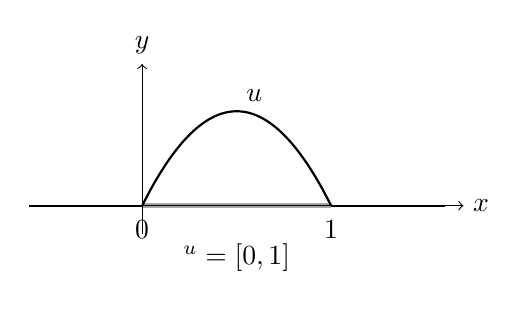
\begin{tikzpicture}[scale=1.2]
            \draw[->] (-1.2,0) -- (3.4,0) node[right] {$x$};
            \draw[->] (0,-0.3) -- (0,1.5) node[above] {$y$};
            \draw[thick, domain=0:1, smooth, variable=\t] plot ({2*\t}, {4*\t*(1-\t)});
            \draw[thick] (-1.2,0) -- (0,0);
            \draw[thick] (2,0) -- (3.2,0);
            \draw[line width=2pt, opacity=0.35] (0,0) -- (2,0);
            \node[below] at (0,-0.05) {$0$};
            \node[below] at (2,-0.05) {$1$};
            \node[above right] at (1,1) {$u$};
            \node[below] at (1,-0.3) {$\sp u=[0,1]$};
        \end{tikzpicture}
    \end{center}
\end{ex}

\begin{lm}\label{lem:bump}
    There is a nonnegative $\phi\in C_c^\infty(\R^n)$ with $\phi(0)>0$.
\end{lm}
\begin{proof}
    Let $f(t)=e^{-1/t}$ for $t>0$ and $f(t)=0$ for $t\le0$.
    By induction, $f^{(k)}(t)=P_k(1/t)e^{-1/t}$ for $t>0$, with polynomials $P_0=1$ and $P_{k+1}(s)=s^2(P_k(s)-P_k'(s))$.
    Since $s^me^{-s}\to0$ as $s\to+\infty$, each $f^{(k)}(t)\to0$ as $t\to0^+$, and inductively $f^{(k)}(0)=0$; hence $f\in C^\infty(\R)$.
    Then $\phi(x)=f(1-\abs x^2)$ is smooth, nonnegative, positive exactly on $\set{\abs x<1}$, and $\phi(0)=e^{-1}$.
\end{proof}

\begin{df}\label{def:compactly-contained}
    Let $A,B$ be subsets of $\R^n$ with $A\subset B$.
    We write $A\Subset B$ if $\bar A$ is a compact subset of $B$.
\end{df}

\begin{remark}\label{rmk:compact-support}
    Let $f\in C^k(X)$.
    Then $f\in C_c^k(X)$ if and only if $\sp f\Subset X$.
    Indeed, if $\sp f$ is a compact subset of $X$, then it is closed in $\R^n$, so $\overline{\sp f}=\sp f$ is a compact subset of $X$.
    Conversely, if the closure $\overline{\sp f}$ in $\R^n$ is a compact subset of $X$, then $\sp f=\overline{\sp f}\cap X=\overline{\sp f}$ is compact.
\end{remark}

\begin{remark}\label{rmk:scaled-bump}
    Let $\phi$ be as in Lemma \ref{lem:bump}, and let $x_0\in\R^n$, $\delta>0$.
    Let $F$ be defined by
    \begin{align*}
        F(x) = \phi\gen*{\frac{x-x_0}{\delta}}.
    \end{align*}
    Then $F\in C_c^\infty(\R^n)$, $F\ge0$, $F(x_0)>0$, and $F$ has support in the closed ball $\bar B_\delta(x_0)$, where $B_\delta(x_0) = \set{x\in\R^n \mid \abs{x-x_0}<\delta}$.
    In particular, if $x_0\in X$, then $F\in C_c^\infty(X)$ for all sufficiently small $\delta>0$.
    (So by translation and scaling we get test functions which are positive at a prescribed point and supported in a prescribed neighborhood of it.)
\end{remark}

\begin{df}\label{def:convolution}
    Let $u,v\in C^0(\R^n)$.
    If $u$ or $v$ has compact support, then the \textit{convolution} $u\ast v$ is the function given by
    \begin{align*}
        (u\ast v)(x) = \int_{\R^n} u(x-y)v(y)\d y.
    \end{align*}
\end{df}

\begin{remark}\label{rmk:convolution-continuous}
    The substitution $y\mapsto x-y$ shows $u\ast v=v\ast u$, so we may assume $v$ has compact support; then the integrand is continuous and vanishes outside $\sp v$, so the integral is well defined.
    Moreover, $u\ast v$ is continuous: if $x_j\to x$ with $\abs{x_j-x}\le1$, then $\abs{u(x_j-y)v(y)}\le C1_{\sp v}(y)$ with $C=\sup_{\bar B_1(x)-\sp v}\abs u\cdot\sup\abs v<+\infty$, and Lebesgue's dominated convergence theorem (Theorem \ref{thm:dct}) applies.
    If both $u$ and $v$ have compact support, then $\sp(u\ast v)\subset\sp u+\sp v$, which is compact.
\end{remark}

\begin{df}\label{def:Lp-loc}
    Let $0<p<+\infty$.
    Define
    \begin{align*}
        L_\loc^p(X) \coloneqq
        \set*{f\colon X\to\bar\R: \text{measurable} \MID \int_K \abs{f}^p <+\infty \text{ for all } K\Subset X}
    \end{align*}
\end{df}

\begin{remark}\label{rmk:convolution-Lloc}
    For $u\in C_c^0(\R^n)$ and $v\in L_\loc^1(\R^n)$, we can also define
    \begin{align*}
        (u\ast v)(x) = \int_{\R^n}u(x-y)v(y)\d y.
    \end{align*}
    Again, $u\ast v$ is continuous by Theorem \ref{thm:dct}: for $\abs{x_j-x}\le1$ the integrands are dominated by $\sup\abs u\cdot\abs{v}1_{S}$, where $S=\bar B_1(x)-\sp u$ is compact and $v\in L^1(S)$.
\end{remark}

\begin{lm}\label{lem:convolution-properties}
\hfill
\begin{enumerate}
    \item
    If $u,v,w\in C_c^0(\R^n)$, then $(u\ast v)\ast w = u\ast (v\ast w)$.

    \item
    If $u\in C_c^j(\R^n)$ and $v\in C^k(\R^n)$, then $u\ast v\in C^{j+k}(\R^n)$ and for all $\alpha,\beta\in\N_0^n$ with $\abs{\alpha}\le j$ and $\abs{\beta}\le k$, one has $\pr_x^\alpha\pr_x^\beta(u\ast v) = (\pr_x^\alpha u)\ast (\pr_x^\beta v)$.

    \item
    If $u\in C_c^j(\R^n)$ and $v\in L_\loc^1(\R^n)$, then $u\ast v\in C^j(\R^n)$ and $\pr_x^\alpha(u\ast v)=(\pr_x^\alpha u)\ast v$ for all $\abs\alpha\le j$.
\end{enumerate}
\end{lm}
\begin{proof}
    (i) Both sides equal $\int\int u(x-y-z)v(z)w(y)\d z\d y$: the integrand is continuous and vanishes outside the compact set $\sp w\times\sp v$, so Fubini's theorem (Theorem \ref{thm:fubini-2}) allows exchanging the order of integration after substituting $z=s-y$.

    (iii) Let $u\in C_c^1$ and $0<\abs h\le1$.
    The difference quotient $\frac1h\left(u(x+he_i-y)-u(x-y)\right)v(y)$ vanishes outside the compact set $S=\bar B_1(x)-\sp u$, is bounded by $\sup\abs{\pr_{x_i}u}\cdot\abs{v(y)}$, and tends to $\pr_{x_i}u(x-y)v(y)$.
    By Theorem \ref{thm:dct}, $\pr_{x_i}(u\ast v)=(\pr_{x_i}u)\ast v$, which is continuous by Remark \ref{rmk:convolution-Lloc}.
    Iterate, using $\pr^\alpha u\in C_c^{j-\abs\alpha}$.

    (ii) The same argument with the roles of $u$ and $v$ exchanged gives $\pr^\beta(u\ast v)=u\ast\pr^\beta v$ for $\abs\beta\le k$.
    Applying (iii) to $u$ and $\pr^\beta v\in C^0\subset L^1_\loc$ gives $\pr^\alpha\pr^\beta(u\ast v)=(\pr^\alpha u)\ast(\pr^\beta v)$, which is continuous.
    Every $\gamma$ with $\abs\gamma\le j+k$ splits as $\alpha+\beta$ with $\abs\alpha\le j$, $\abs\beta\le k$, so $u\ast v\in C^{j+k}$.
\end{proof}

Let $\chi\in C_c^\infty(\R^n)$ be the function such that $\chi\ge 0$, $\sp\chi \subset B_1(0)$, and $\int_{\R^n}\chi = 1$.
(Such a function exists: take $\phi$ from Lemma \ref{lem:bump}, put $\chi(x)=c\,\phi(2x)$ with $c=\left(\int\phi(2x)\d x\right)^{-1}$; then $\sp\chi=\bar B_{1/2}(0)\subset B_1(0)$.)
For any $\eps>0$, let $\chi_\eps(x) = \eps^{-n}\chi(x/\eps)\in C_c^\infty(B_\eps(0))$.
Note that $\int_{\R^n}\chi_\eps(x)\d x=1$.

\begin{thm}\label{thm:mollification}
    Fix $j\in\N_0$ and let $u\in C_c^j(\R^n)$.
    Define $u_\eps\coloneqq u\ast \chi_\eps\in C_c^\infty(\R^n)$.
    Then
    \begin{align*}
        \lim_{\eps\to 0} \sup\set{\abs{\pr_x^\alpha(u_\eps-u)(x)} \mid x\in \R^n,\, \abs{\alpha}\le j} = 0.
    \end{align*}
\end{thm}
\begin{proof}
    By Lemma \ref{lem:convolution-properties}(ii) and Remark \ref{rmk:convolution-continuous}, $u_\eps\in C_c^\infty(\R^n)$ and $\pr^\alpha u_\eps=(\pr^\alpha u)\ast\chi_\eps$ for $\abs\alpha\le j$.
    Since $\chi_\eps\ge0$, $\int\chi_\eps=1$ and $\chi_\eps=0$ outside $B_\eps(0)$,
    \begin{align*}
        \abs{\pr^\alpha(u_\eps-u)(x)}
        =\abs*{\int_{\R^n}\left(\pr^\alpha u(x-y)-\pr^\alpha u(x)\right)\chi_\eps(y)\d y}
        \le\sup_{\abs y\le\eps}\abs{\pr^\alpha u(x-y)-\pr^\alpha u(x)},
    \end{align*}
    which tends to $0$ uniformly in $x$, because $\pr^\alpha u$ is continuous with compact support, hence uniformly continuous.
\end{proof}

\begin{thm}\label{thm:cutoff}
    Let $K\Subset X$.
    Then there exists a function $\phi\in C_c^\infty(X)$ with $0\le\phi\le 1$ such that $\phi\equiv 1$ in some neighborhood of $K$.
\end{thm}
\begin{proof}
    Let $K_\delta=\set{x\mid\operatorname{dist}(x,K)<\delta}$, and choose $\eps>0$ with $\operatorname{dist}(K,\R^n\setminus X)\ge4\eps$.
    Put $\phi=1_{K_{2\eps}}\ast\chi_\eps$, which is smooth by Lemma \ref{lem:convolution-properties}(iii) and takes values in $[0,1]$.
    Since $\chi_\eps=0$ outside $B_\eps(0)$: if $x\notin K_{3\eps}$, then $x-y\notin K_{2\eps}$ for $\abs y<\eps$, so $\phi(x)=0$; and if $x\in K_\eps$, then $x-y\in K_{2\eps}$ for $\abs y<\eps$, so $\phi(x)=\int\chi_\eps=1$.
    Hence $\phi\equiv1$ on $K_\eps$, and $\sp\phi\subset\overline{K_{3\eps}}$ is a compact subset of $X$.
\end{proof}

\begin{thm}[Partition of unity]\label{thm:partition-of-unity}
    Let $X_1,\dots, X_k$ be open sets in $\R^n$.
    Then given $\phi\in C_c^\infty(\bigcup_{j=1}^{k} X_j)$, there exists $\phi_j\in C_c^\infty(X_j)$ for each $j$ such that $\phi = \phi_1 + \cdots + \phi_k$.
    If $\phi\ge0$, we can take all $\phi_j\ge0$.
\end{thm}
\begin{proof}
    By compactness, $\sp\phi$ is covered by finitely many closed balls, each contained in some $X_j$; let $K_j\Subset X_j$ be the union of those assigned to $X_j$, so $\sp\phi\subset\bigcup_jK_j$.
    By Theorem \ref{thm:cutoff}, take $\psi_j\in C_c^\infty(X_j)$ with $0\le\psi_j\le1$ and $\psi_j\equiv1$ near $K_j$ ($\psi_j=0$ if $K_j=\varnothing$).
    With $P_j=(1-\psi_1)\cdots(1-\psi_j)$ and $P_0=1$, put
    \begin{align*}
        \phi_j=\phi P_{j-1}\psi_j=\phi(P_{j-1}-P_j)\in C_c^\infty(X_j).
    \end{align*}
    The sum telescopes to $\phi-\phi P_k$, and $\phi P_k=0$ since every point of $\sp\phi$ lies in some $K_j$, where $\psi_j=1$.
    If $\phi\ge0$, then each $\phi_j\ge0$.
\end{proof}

\begin{df}\label{def:distribution}
    A \textit{distribution} in $X$ is a linear functional $u$ from the space of test functions $C_c^\infty(X)$ to $\C$ such that for every $K\Subset X$, there exist constants $C>0$ and $k\in\N_0$ such that
    \begin{align*}
        \abs{u(\phi)}
        \le C\sum_{\abs{\alpha}\le k} \sup_{\R^n} \abs{\pr_x^\alpha \phi}
    \end{align*}
    for all $\phi\in C_c^\infty(X)$ with $\sp\phi\subset K$.
    Note that $C$ and $k$ depend only on $K$.
    The space of all distributions is denoted by $\mathcal D'(X)$.
\end{df}

\begin{ex}\label{ex:L1loc-distribution}
    Let $u\in L_\loc^1(X)$.
    Then the linear functional $T_u\colon C_c^\infty(X)\to \C$ defined by
    \begin{align*}
        T_u(\phi) = \int_{X} u\phi
    \end{align*}
    is a distribution.
    Indeed, $T_u$ is well defined and linear because $u\phi$ is integrable (as $\sp\phi\Subset X$), and for every $K\Subset X$ and every $\phi\in C_c^\infty(X)$ with $\sp\phi\subset K$,
    \begin{align*}
        \abs{T_u(\phi)}\le\int_K\abs u\abs\phi\le\left(\int_K\abs u\right)\sup_{\R^n}\abs\phi.
    \end{align*}
    So the condition holds with $C=\max\set{\int_K\abs u,1}$ and $k=0$.
\end{ex}

\begin{ex}\label{ex:dirac}
    Let $p\in X$.
    The \textit{Dirac distribution} $\delta_p\in\mathcal D'(X)$ is defined by
    \begin{align*}
        \delta_p \colon
        \begin{array}{ccc}
            C_c^\infty(X) & \to & \C \\
            \phi & \mapsto & \phi(p)
        \end{array}.
    \end{align*}
    It is clearly linear, and $\abs{\delta_p(\phi)}=\abs{\phi(p)}\le\sup_{\R^n}\abs\phi$ for all $\phi\in C_c^\infty(X)$, so $\delta_p$ is a distribution with $C=1$ and $k=0$ for every $K\Subset X$.
    This is important in the theory of PDE.
\end{ex}


\newpage
\subsection{20261110}\label{ssec:1110}
\begin{thm}\label{thm:smooth-dependence}
    Let $\phi\in C_c^\infty(X\times Y)$, where $X\subset \R^n$ and $Y\subset\R^m$ are open sets.
    Let $u\in \mathcal D'(X)$.
    Then the function $y\in Y\mapsto u(\phi(\cdot,y))$ is a smooth function in $Y$, and
    \begin{align*}
        \pr_y^\alpha\, u(\phi(\cdot,y)) = u(\pr_y^\alpha\phi(\cdot,y))
    \end{align*}
    for all $\alpha\in \N_0^m$.
\end{thm}
\begin{proof}
    The projection $K$ of $\sp\phi$ to $X$ is compact, and $\sp\phi(\cdot,y)\subset K$ for all $y$; the same holds for every $\pr_y^\alpha\phi$.
    Fix $y$ and small $h\in\R^m$.
    By Taylor's formula,
    \begin{align*}
        \phi(x,y+h)=\phi(x,y)+\sum_{j=1}^{m}h_j\frac{\pr\phi}{\pr y_j}(x,y)+\Psi(x,y,h),\quad
        \Psi=\sum_{i,j=1}^{m}h_ih_j\int_0^1(1-t)\frac{\pr^2\phi}{\pr y_i\pr y_j}(x,y+th)\,dt,
    \end{align*}
    and $\sp\Psi(\cdot,y,h)\subset K$.
    Differentiating under the integral sign in $x$ and using $\abs{h_ih_j}\le\abs h^2$ and $\int_0^1(1-t)\,dt=\frac12$, for every $\beta\in\N_0^n$,
    \begin{align*}
        \sup_x\abs{\pr_x^\beta\Psi(x,y,h)}
        \le\sum_{i,j=1}^{m}\abs h^2\cdot\frac12\sup_{X\times Y}\abs{\pr_x^\beta\pr_{y_i}\pr_{y_j}\phi}
        \le C_\beta\abs h^2,\qquad
        C_\beta\coloneqq\frac{m^2}{2}\max_{i,j}\sup_{X\times Y}\abs{\pr_x^\beta\pr_{y_i}\pr_{y_j}\phi}.
    \end{align*}
    Applying the linear form $u$ to the Taylor expansion,
    \begin{align*}
        u(\phi(\cdot,y+h))=u(\phi(\cdot,y))+\sum_{j=1}^{m}h_j\,u\left(\frac{\pr\phi}{\pr y_j}(\cdot,y)\right)+u(\Psi(\cdot,y,h)),
    \end{align*}
    and by the estimate of Definition \ref{def:distribution} on $K$ (with constants $C,k$),
    \begin{align*}
        \abs{u(\Psi(\cdot,y,h))}\le C\sum_{\abs\beta\le k}\sup_x\abs{\pr_x^\beta\Psi(x,y,h)}\le\Bigl(C\sum_{\abs\beta\le k}C_\beta\Bigr)\abs h^2=O(\abs h^2).
    \end{align*}
    So $y\mapsto u(\phi(\cdot,y))$ is differentiable with $\pr_{y_j}u(\phi(\cdot,y))=u(\pr_{y_j}\phi(\cdot,y))$.
    Since $\pr_{y_j}\phi\in C_c^\infty(X\times Y)$ again, induction gives all derivatives, each of which is differentiable, hence continuous.
\end{proof}

\begin{remark}\label{rmk:differentiation-under-integral}
    Let $E\subset \R^n$ be any measurable set.
    Then the linear functional $u\colon C_c^\infty(\R^n)\to\C$ defined by
    \begin{align*}
        u(f) = \int_E f(x)\d x
    \end{align*}
    is a distribution, i.e.\ $u\in \mathcal D'(\R^n)$: it is $T_{1_E}$ from Example \ref{ex:L1loc-distribution}, as $1_E\in L^1_\loc(\R^n)$.
    Let $\phi(x,y)\in C_c^\infty(\R^n\times\R^n)$.
    Then
    \begin{align*}
        u(\phi(\cdot,y)) = \int_E \phi(x,y)\d x.
    \end{align*}
    Theorem \ref{thm:smooth-dependence} then says that $y\mapsto\int_E\phi(x,y)\d x$ is a smooth function in $y\in\R^n$, and
    \begin{align*}
        \pr_y^\alpha \int_E \phi(x,y)\d x
        = \pr_y^\alpha u(\phi(\cdot,y))
        = u(\pr_y^\alpha\phi(\cdot,y))
        = \int_E (\pr_y^\alpha\phi)(x,y)\d x
    \end{align*}
    for all $\alpha\in\N_0^n$.
    (This is differentiation under the integral sign.)
\end{remark}

\begin{df}[Topology on $C_c^\infty(X)$]\label{def:test-function-convergence} % Direct limit topology
    Let $\phi,\phi_j\in C_c^\infty(X)$.
    We say that the sequence $\phi_j$ \textit{converges to} $\phi$ \textit{in} $C_c^\infty(X)$ if there exists $K\Subset X$ such that $\sp \phi_j\subset K$ for all $j$, $\sp\phi\subset K$, and
    \begin{align*}
        \lim_{j\to+\infty} \sup_{x\in X} \abs{(\pr_x^\alpha(\phi_j-\phi))(x)} = 0
    \end{align*}
    for all $\alpha\in\N_0^n$.
    (This is the topology of the direct limit, i.e.\ the union, of the spaces $\set{\phi\in C_c^\infty(X)\mid\sp\phi\subset K}$ over $K\Subset X$.)
\end{df}

\begin{thm}\label{thm:sequential-continuity}
    Let $u\colon C_c^\infty(X)\to\C$ be a linear form.
    Then $u$ is a distribution if and only if $\lim_{j\to+\infty} u(\phi_j) = u(\phi)$ for any sequence $\phi_j\in C_c^\infty(X)$ converging to $\phi\in C_c^\infty(X)$ in $C_c^\infty(X)$.
    In other words, $u\in \mathcal D'(X)$ if and only if $u$ is (sequentially) continuous in the topology of $C_c^\infty(X)$.
\end{thm}
\begin{proof}
    \textit{Only if}: if $\phi_j\to\phi$ with supports in $K$, the estimate of Definition \ref{def:distribution} on $K$ gives $\abs{u(\phi_j)-u(\phi)}\le C\sum_{\abs\alpha\le k}\sup\abs{\pr^\alpha(\phi_j-\phi)}\to0$.

    \textit{If}: suppose the estimate fails on some $K\Subset X$.
    Then for each $j$ (taking $C=k=j$) there is $\phi_j$ with $\sp\phi_j\subset K$ and $\abs{u(\phi_j)}>j\sum_{\abs\alpha\le j}\sup\abs{\pr^\alpha\phi_j}$.
    In particular $u(\phi_j)\ne0$; since the inequality is homogeneous in $\phi_j$, we may replace $\phi_j$ by $\phi_j/\abs{u(\phi_j)}$ and assume $\abs{u(\phi_j)}=1$.
    Then
    \begin{align*}
        \sum_{\abs\alpha\le j}\sup_X\abs{\pr^\alpha\phi_j}<\frac1j,
        \quad\text{so}\quad
        \sup_X\abs{\pr^\alpha\phi_j}<\frac1j\to0\quad\text{for every fixed }\alpha\text{ and all }j\ge\abs\alpha.
    \end{align*}
    As all $\phi_j$ are supported in $K$, this means $\phi_j\to0$ in $C_c^\infty(X)$, so continuity gives $u(\phi_j)\to u(0)=0$, contradicting $\abs{u(\phi_j)}=1$.
\end{proof}

\begin{df}[Topology in $\mathcal D'(X)$]\label{def:distribution-convergence}
    Let $u,u_j\in\mathcal D'(X)$.
    We say that the sequence $u_j$ \textit{converges to} $u$ \textit{in} $\mathcal D'(X)$ if $u_j(\phi)\to u(\phi)$ for every $\phi\in C_c^\infty(X)$.
\end{df}

In functional analysis, this is called the \textit{weak-$^\ast$ topology}.

\begin{thm}[Completeness of $\mathcal D'(X)$]\label{thm:distribution-completeness}
    Let $u_j\in\mathcal D'(X)$.
    Suppose that $\lim_{j\to+\infty} u_j(\phi)$ exists for all $\phi\in C_c^\infty(X)$.
    Then the linear form
    \begin{align*}
        u\colon
        \begin{array}{ccc}
            C_c^\infty(X) & \to & \C  \\
            \phi & \mapsto & u(\phi)\coloneqq \lim_{j\to+\infty} u_j(\phi)
        \end{array}
    \end{align*}
    is a distribution.
    Moreover, for every $K\Subset X$, there exist $C>0$ and $k\in\N_0$, \textit{independent of} $j$, such that
    \begin{align}\label{eq:uniform-bound}
        \abs{u_j(\phi)} \le C\sum_{\abs{\alpha}\le k}\sup_X \abs{(\pr_x^\alpha\phi)(x)}
    \end{align}
    for all $\phi\in C_c^\infty(X)$ with $\sp\phi\subset K$ and for all $j\in\N$.
\end{thm}

\begin{remark}\label{rmk:uniform-boundedness}
    Theorem \ref{thm:distribution-completeness} can be proven by the concept of uniform boundedness and the Baire--Hausdorff method in functional analysis (these two important principles of functional analysis stand behind this proof; they will be introduced in this week's homework).
    We will give a direct proof by contradiction.
\end{remark}

\begin{proof}
    Letting $j\to+\infty$ in \eqref{eq:uniform-bound} shows that $u$ is a distribution, so it suffices to prove \eqref{eq:uniform-bound}.
    Fix $K$, write $p_k(\phi)=\sum_{\abs\alpha\le k}\sup_X\abs{\pr^\alpha\phi}$ (increasing in $k$), and suppose that for every $C,k$ there are $\ell$ and $\phi$ with $\sp\phi\subset K$ and $\abs{u_\ell(\phi)}>C\,p_k(\phi)$; such $\phi$ may be rescaled freely.

    \textit{Claim: there are $\ell_1<\ell_2<\cdots$, $k_1<k_2<\cdots$ and $\phi_j$ with $\sp\phi_j\subset K$ such that}
    \begin{enumerate}
        \item $p_{k_j}(\phi_j)\le 2^{-j}$,
        \item $\abs{u_{\ell_j}(\phi_j)} - \abs{u_{\ell_j}(\phi_1)} - \cdots - \abs{u_{\ell_j}(\phi_{j-1})} \ge j$, and
        \item $\abs{u_{\ell_i}(\phi_j)} < 2^{-j}$ for all $i<j$.
    \end{enumerate}
    For $j=1$, take $\abs{u_{\ell_1}(\phi_1)}>2p_1(\phi_1)$, normalized to $\abs{u_{\ell_1}(\phi_1)}=1$, and $k_1=1$.
    Given the first $j_0$ terms, the finitely many $u_\ell$ with $\ell\le\ell_{j_0}$ satisfy a common estimate
    \begin{align}\label{eq:finite-bound}
        \abs{u_\ell(\phi)}\le\hat C\,p_{\hat k}(\phi)\qquad(\sp\phi\subset K,\ \ell\le\ell_{j_0}),
    \end{align}
    and $M=\sum_{i\le j_0}\sup_\ell\abs{u_\ell(\phi_i)}<+\infty$ since convergent sequences are bounded.
    Let $a=j_0+1+M$, $C'=(a+\hat C)^22^{j_0+1}$, $L=\max\set{k_{j_0}+1,\hat k}$, and pick $\ell,\phi$ with $\abs{u_\ell(\phi)}>C'p_L(\phi)$, rescaled so that $\abs{u_\ell(\phi)}=a$.
    If $\ell\le\ell_{j_0}$, then \eqref{eq:finite-bound} would give $\abs{u_\ell(\phi)}\le\hat C\,p_{\hat k}(\phi)\le\hat C\,p_L(\phi)\le C'p_L(\phi)$, a contradiction; so $\ell>\ell_{j_0}$.
    Set $\ell_{j_0+1}=\ell$, $k_{j_0+1}=L$ and $\phi_{j_0+1}=\phi$, and check (i)--(iii) for $j=j_0+1$:
    \begin{align*}
        \text{(i)}\quad & p_{k_{j_0+1}}(\phi_{j_0+1})<\frac{\abs{u_\ell(\phi)}}{C'}=\frac{a}{(a+\hat C)^2}\,2^{-j_0-1}\le\frac1a\,2^{-j_0-1}<2^{-j_0-1}, \\
        \text{(ii)}\quad & \abs{u_{\ell_{j_0+1}}(\phi_{j_0+1})}-\sum_{i=1}^{j_0}\abs{u_{\ell_{j_0+1}}(\phi_i)}\ge a-M=j_0+1, \\
        \text{(iii)}\quad & \abs{u_{\ell_i}(\phi_{j_0+1})}\le\hat C\,p_L(\phi_{j_0+1})<\frac{\hat C\,a}{(a+\hat C)^2}\,2^{-j_0-1}\le\frac14\,2^{-j_0-1}<2^{-(j_0+1)}\quad(i\le j_0),
    \end{align*}
    where (iii) uses \eqref{eq:finite-bound} (as $\ell_i\le\ell_{j_0}$) and $(a+\hat C)^2\ge4a\hat C$.

    Now put $\phi=\sum_j\phi_j$.
    Since $k_j\ge j$, (i) gives $\sum_jp_N(\phi_j)<+\infty$ for every $N$, so the series converges in $C_c^\infty(X)$ with $\sp\phi\subset K$, and by Theorem \ref{thm:sequential-continuity}, $u_{\ell_j}(\phi)=\sum_iu_{\ell_j}(\phi_i)$.
    Splitting this sum into $i=j$, $i<j$ and $i>j$, and using (ii) and (iii) (with the roles $\ell_j$, $i=j+s$),
    \begin{align*}
        \abs{u_{\ell_j}(\phi)}
        &\ge\abs{u_{\ell_j}(\phi_j)}-\sum_{i=1}^{j-1}\abs{u_{\ell_j}(\phi_i)}-\sum_{s=1}^{+\infty}\abs{u_{\ell_j}(\phi_{j+s})}\\
        &\ge j-\sum_{s=1}^{+\infty}2^{-(j+s)}\ge j-1\to+\infty,
    \end{align*}
    contradicting the convergence, hence boundedness, of $(u_\ell(\phi))_\ell$.
\end{proof}


\newpage
\subsection{20261112}\label{ssec:1112}
\begin{df}\label{def:distribution-derivative}
    Let $u\in\mathcal D'(X)$.
    For $k=1,2,\dots,n$, let $\pr u/\pr x_k$ be the distribution given by
    \begin{align*}
        \frac{\pr u}{\pr x_k}(\phi) = -u\gen*{\frac{\pr\phi}{\pr x_k}}.
    \end{align*}
    For $f\in C^\infty(X)$, let $f.u$ be the distribution given by
    \begin{align*}
        f.u(\phi) = u(f\phi).
    \end{align*}
\end{df}

\begin{lm}\label{lem:derivative-product-distribution}
    The linear forms $\pr u/\pr x_k$ and $f.u$ in Definition \ref{def:distribution-derivative} are indeed distributions.
\end{lm}
\begin{proof}
    Both are well defined and linear, since $\pr_{x_k}\phi,f\phi\in C_c^\infty(X)$ with support in $\sp\phi$.
    Let $K\Subset X$, and let $C,k_0$ be the constants of $u$ on $K$.
    For $\sp\phi\subset K$, apply the estimate to $\pr_{x_k}\phi$; each $\pr^\alpha\pr_{x_k}$ with $\abs\alpha\le k_0$ is some $\pr^\beta$ with $\abs\beta\le k_0+1$, so
    \begin{align*}
        \abs*{\frac{\pr u}{\pr x_k}(\phi)}=\abs*{u\gen*{\frac{\pr\phi}{\pr x_k}}}
        \le C\sum_{\abs\alpha\le k_0}\sup\abs{\pr^\alpha\pr_{x_k}\phi}
        \le C\sum_{\abs\beta\le k_0+1}\sup\abs{\pr^\beta\phi}.
    \end{align*}
    For $f.u$, let $A=\max_{\abs\beta\le k_0}\sup_K\abs{\pr^\beta f}<+\infty$.
    By the Leibniz rule $\pr^\alpha(f\phi)=\sum_{\beta\le\alpha}\binom\alpha\beta\pr^\beta f\,\pr^{\alpha-\beta}\phi$ and $\sum_{\beta\le\alpha}\binom\alpha\beta=2^{\abs\alpha}$, for $\abs\alpha\le k_0$,
    \begin{align*}
        \sup\abs{\pr^\alpha(f\phi)}
        \le\sum_{\beta\le\alpha}\binom\alpha\beta\sup_K\abs{\pr^\beta f}\,\sup\abs{\pr^{\alpha-\beta}\phi}
        \le2^{k_0}A\sum_{\abs\gamma\le k_0}\sup\abs{\pr^\gamma\phi},
    \end{align*}
    and summing over the $\abs\alpha\le k_0$ in the estimate for $u(f\phi)$,
    so $f.u$ satisfies the estimate with $C'=C\cdot\#\set{\alpha\mid\abs\alpha\le k_0}\cdot2^{k_0}A$ (or $1$ if this vanishes).
\end{proof}

\begin{ex}\label{ex:distributional-derivative}
    Let $f\in L_\loc^1(X)$.
    Then $T_f$, the function given by
    \begin{align*}
        T_f(\phi) = \int_{X}f(x)\phi(x)\d x,
    \end{align*}
    is a distribution (Example \ref{ex:L1loc-distribution}).
    We sometimes write $f$ to represent $T_f$.
    Note that if $f\in C^1(X)$, then
    \begin{align*}
        \frac{\pr T_f}{\pr x_k} (\phi)
        = -\int_{X}f(x) \frac{\pr\phi}{\pr x_k}\d x
        = \int_X \frac{\pr f}{\pr x_k}\phi(x)\d x
        = T_{\pr f/\pr x_k}(\phi).
    \end{align*}
    The middle equality is integration by parts: extend $f\phi$ by zero to a compactly supported $C^1$ function $g$ on $\R^n$; then $\int_{\R^n}\pr_{x_k}g\,dx=0$ by Fubini's theorem (Theorem \ref{thm:fubini-2}) and the fundamental theorem of calculus in the variable $x_k$, and $\pr_{x_k}(f\phi)=\pr_{x_k}f\cdot\phi+f\cdot\pr_{x_k}\phi$.
    So the distributional derivative of $T_f$ is $T_{\pr f/\pr x_k}$, the distribution of the classical derivative.
\end{ex}

\begin{remark}\label{rmk:continuous-identification}
    The identification $f=T_f$ is legitimate for continuous functions: if $f,g\in C^0(X)$ and $T_f=T_g$, then $f=g$.
    Indeed, let $h=f-g$ and suppose $h(x_0)\ne0$ for some $x_0$.
    Choose $c\in\C$ with $\abs c=1$ and $\operatorname{Re}(ch(x_0))>0$; by continuity, $\operatorname{Re}(ch)>\eta>0$ on some ball $B_\rho(x_0)\subset X$.
    Let $F(x)=\phi((x-x_0)/\delta)$ with $\phi$ from Lemma \ref{lem:bump} and $\delta<\rho$ small; then $F\ge0$, $F\not\equiv0$, $F\in C_c^\infty(B_\rho(x_0))$.
    So $\operatorname{Re}(c\,T_h(F))=\int\operatorname{Re}(ch)F\ge\eta\int F>0$, contradicting $T_h=0$.
    (More generally, for $f,g\in L^1_\loc(X)$ one has $T_f=T_g$ if and only if $f=g$ almost everywhere; we do not need this.)
\end{remark}

\begin{ex}\label{ex:heaviside}
    Consider the Heaviside function
    \begin{align*}
        H(x) =
        \begin{cases}
            1 & \text{if } x\ge 0 \\
            0 & \text{if } x<0
        \end{cases}.
    \end{align*}
    It is clear that $H\in L_\loc^1(\R)$.
    For $\phi\in C_c^\infty(\R)$, say $\sp\phi\subset[-R,R]$, we have
    \begin{align*}
        \frac{\pr T_H}{\pr x}(\phi)
        = -T_H\gen*{\frac{\pr\phi}{\pr x}}
        = -\int_{0}^{+\infty} \frac{\pr\phi}{\pr x}\d x
        = -\left(\phi(R)-\phi(0)\right)
        = \phi(0)
        = \delta_0(\phi),
    \end{align*}
    so $T_H' = \delta_0$.
    That is, the derivative of the Heaviside function is the delta distribution (Example \ref{ex:dirac}), even though $H$ is not differentiable at $0$ in the classical sense.
\end{ex}

\begin{ex}\label{ex:indicator-derivative}
    Let $Y=\set{x\in\R^n\mid r(x)<0}$, where $r\in C^1(\R^n)$ and $\nabla r(x) \ne 0$ on $\pr Y= \set{x\in\R^n\mid r(x)=0}$.
    By the implicit function theorem, $\pr Y$ is a $C^1$ hypersurface and $Y$ lies locally on one side of it.
    We compute the derivative of $T_{1_Y}= 1_Y\in L^1_\loc(\R^n)$:
    Let $N=(N_1,\dots,N_n)$ be the inward normal vector of $\pr Y$, that is, $N=-\nabla r/\abs{\nabla r}$, and let $\d S$ be the volume form (surface measure) on $\pr Y$.
    For $\phi\in C_c^\infty(\R^n)$, the Gauss--Green theorem (Example \ref{ex:gauss-green}), applied to the compactly supported vector field $\phi\, e_k$ on $Y$ (whose outward normal is $-N$), gives $\int_Y\pr_{x_k}\phi\,dx=-\int_{\pr Y}N_k\phi\d S$.
    Hence
    \begin{align*}
       \frac{\pr 1_Y}{\pr x_k} (\phi)
        = - 1_Y\gen*{\frac{\pr\phi}{\pr x_k}}
        = -\int_Y \frac{\pr\phi}{\pr x_k}\d x
        = \int_{\pr Y} N_k\phi\d S.
    \end{align*}
    Therefore,
    \begin{align*}
        \frac{\pr 1_Y}{\pr x_k} = N_k \,.\, \delta_{\pr Y},
    \end{align*}
    where $\delta_{\pr Y}$ is the distribution sending $\phi\in C_c^\infty(\R^n)$ to $\int_{\pr Y}\phi\d S$, and $N_k\delta_{\pr Y}$ is the distribution $\phi\mapsto\int_{\pr Y}N_k\phi\d S$.
    (These are distributions of order $0$: $\abs{\int_{\pr Y}N_k\phi\d S}\le\operatorname{area}(\pr Y\cap K)\sup\abs\phi$ if $\sp\phi\subset K$, and $\operatorname{area}(\pr Y\cap K)<+\infty$ since $\pr Y\cap K$ is compact.)
    For $n=1$ and $r(x)=-x$, we have $Y=(0,+\infty)$, $N=1$, $\delta_{\pr Y}=\delta_0$, and we recover $T_H'=\delta_0$ (Example \ref{ex:heaviside}).
\end{ex}

\begin{df}\label{def:distribution-restriction}
    Let $U\subset X$ be an open set.
    Every $\phi\in C_c^\infty(U)$ extends by zero to an element of $C_c^\infty(X)$, so we regard $C_c^\infty(U)\subset C_c^\infty(X)$.
    For $u\in\mathcal D'(X)$, we denote by $u|_{U}\in\mathcal D'(U)$ the restriction of $u$ to $C_c^\infty(U)$.
    (It is a distribution: a compact subset of $U$ is a compact subset of $X$, so the estimate for $u$ gives the same estimate for $u|_U$.)
    We say that $u$ \textit{vanishes on} $U$ if $u|_U=0$, that is, if $u(\phi)=0$ for all $\phi\in C_c^\infty(U)$.
\end{df}

\begin{thm}[Localization]\label{thm:localization}
    Let $u\in\mathcal D'(X)$.
    If for every $p\in X$, there exists an open neighborhood $U_p\subset X$ such that $u|_{U_p}=0$, then $u=0$.
\end{thm}
\begin{proof}
    Let $\phi\in C_c^\infty(X)$.
    Finitely many of the $U_p$, say $U_1,\dots,U_N$, cover $\sp\phi$.
    By Theorem \ref{thm:partition-of-unity}, $\phi=\sum_j\phi_j$ with $\phi_j\in C_c^\infty(U_j)$, so $u(\phi)=\sum_ju|_{U_j}(\phi_j)=0$.
\end{proof}

\begin{df}\label{def:distribution-support}
    Let $u\in\mathcal D'(X)$.
    The support of $u$, denoted by $\sp u$, is the set of points $p$ in $X$ such that $u|_{U_p}\ne 0$ for every open neighborhood $U_p\subset X$.
    That is,
    \begin{align*}
        X\setminus\sp u=\set{x\in X\mid \text{there is an open set }U_x\subset X\text{ with }x\in U_x\text{ and }u|_{U_x}=0}.
    \end{align*}
\end{df}

\begin{lm}\label{lem:support-closed}
    Let $u\in\mathcal D'(X)$.
    Then $\sp u$ is closed in $X$, and $u$ vanishes on the open set $X\setminus\sp u$.
\end{lm}
\begin{proof}
    If $u|_{U_x}=0$, then every point of $U_x$ lies outside $\sp u$, so $X\setminus\sp u$ is open.
    Every point of $X\setminus\sp u$ has a neighborhood on which $u$ vanishes, so $u|_{X\setminus\sp u}=0$ by Theorem \ref{thm:localization}.
\end{proof}

\begin{df}\label{def:compactly-supported-distributions}
    Let $\mathcal E'(X)$ be the set of $u\in\mathcal D'(X)$ such that $\sp u$ is a compact subset of $X$.
\end{df}

\begin{ex}\label{ex:dirac-support}
    For $p\in X$, let $\delta_p$ be the distribution sending $\phi$ to $\phi(p)$.
    Then $\sp\delta_p = \set{p}$: if $x\ne p$, then $\delta_p$ vanishes on $X\setminus\set p$ (as $\phi(p)=0$ for every $\phi\in C_c^\infty(X\setminus\set p)$), so $x\notin\sp\delta_p$; and every neighborhood $U$ of $p$ contains a test function $F\ge0$ with $F(p)>0$ (Remark \ref{rmk:scaled-bump}), so $\delta_p|_U\ne0$ and $p\in\sp\delta_p$.
    Thus $\delta_p\in\mathcal E'(X)$.
\end{ex}

\begin{ex}\label{ex:test-functions-compact-support}
    Under the identification $f=T_f$, we have $C_c^\infty(X)\subset\mathcal E'(X)$.
    Indeed, if $x\notin\sp f$, then $f$ vanishes on a neighborhood $U$ of $x$, so $T_f|_U=0$ and $x\notin\sp T_f$.
    Hence $\sp T_f\subset\sp f$, and $\sp T_f$ is a closed subset of $X$ contained in the compact set $\sp f$, so it is compact.
\end{ex}

\begin{thm}[Glueing]\label{thm:glueing}
    Let $X_1,X_2,\dots$ be open sets and let $X=\bigcup_{j=1}^{+\infty}X_j$.
    If $u_j\in\mathcal D'(X_j)$ is such that $u_j=u_k$ on $X_j\cap X_k$ for all $j$ and for all $k$ (that is, $u_j|_{X_j\cap X_k}=u_k|_{X_j\cap X_k}$), then there exists a unique $u\in\mathcal D'(X)$ such that $u|_{X_j} = u_j$ for all $j$.
\end{thm}
\begin{proof}
    For $\phi\in C_c^\infty(X)$, Theorem \ref{thm:partition-of-unity} gives a finite decomposition $\phi=\sum_j\phi_j$ with $\phi_j\in C_c^\infty(X_j)$; define $u(\phi)=\sum_ju_j(\phi_j)$.

    \textit{Well-definedness.}
    Let $\phi=\sum_j\tilde\phi_j$ be another such decomposition, and let $K=\bigcup_j\sp(\tilde\phi_j-\phi_j)$, a compact set.
    By Theorems \ref{thm:cutoff} and \ref{thm:partition-of-unity}, there are $\Psi_k\in C_c^\infty(X_k)$, finitely many nonzero, with $\sum_k\Psi_k=1$ near $K$.
    Since $\Psi_k(\tilde\phi_j-\phi_j)\in C_c^\infty(X_j\cap X_k)$ and $u_j=u_k$ there,
    \begin{align*}
        \sum_ju_j(\tilde\phi_j-\phi_j)
        =\sum_{j,k}u_k\bigl(\Psi_k(\tilde\phi_j-\phi_j)\bigr)
        =\sum_ku_k\Bigl(\Psi_k\sum_j(\tilde\phi_j-\phi_j)\Bigr)=0.
    \end{align*}
    Hence $u$ is well defined and linear, and $u|_{X_j}=u_j$ (take the decomposition $\phi=\phi_j$).
    Uniqueness follows from Theorem \ref{thm:localization}.

    \textit{$u$ is a distribution.}
    For $K\Subset X$, take $\varphi_j\in C_c^\infty(X_j)$, finitely many nonzero, with $\sum_j\varphi_j=1$ near $K$, and let $C_j,k_j$ be the constants of $u_j$ on $\sp\varphi_j$.
    Let $J$ be the finite set of $j$ with $\varphi_j\ne0$, $C=\max_{j\in J}C_j$, $k=\max_{j\in J}k_j$ and $A=\max_{j\in J}\max_{\abs\beta\le k}\sup\abs{\pr^\beta\varphi_j}$.
    For $\sp\phi\subset K$ we have $\phi=\sum_{j\in J}\varphi_j\phi$ with $\varphi_j\phi\in C_c^\infty(X_j)$ supported in $\sp\varphi_j$, so by the definition of $u$ and the Leibniz rule (as in Lemma \ref{lem:derivative-product-distribution}),
    \begin{align*}
        \abs{u(\phi)}
        \le\sum_{j\in J}\abs{u_j(\varphi_j\phi)}
        \le\sum_{j\in J}C_j\sum_{\abs\alpha\le k_j}\sup\abs{\pr^\alpha(\varphi_j\phi)}
        \le\#J\cdot C\cdot\#\set{\alpha\mid\abs\alpha\le k}\cdot2^kA\sum_{\abs\gamma\le k}\sup\abs{\pr^\gamma\phi}.
    \end{align*}
\end{proof}

\begin{supp}
    Theorem \ref{thm:localization} and Theorem \ref{thm:glueing} say that the presheaf of distributions is a sheaf.
    Recall the definitions.
    A \textit{presheaf} $\mathcal F$ of vector spaces on a topological space $X$ assigns to every open set $U\subset X$ a vector space $\mathcal F(U)$ and to every pair of open sets $V\subset U$ a linear \textit{restriction map} $\mathcal F(U)\to\mathcal F(V)$, $s\mapsto s|_V$, such that $s|_U=s$ and $(s|_V)|_W=s|_W$ for $W\subset V\subset U$.
    It is a \textit{sheaf} if for every open set $U$ and every open cover $U=\bigcup_{i}U_i$, the following hold.
    \begin{enumerate}
        \item (Locality) If $s\in\mathcal F(U)$ and $s|_{U_i}=0$ for all $i$, then $s=0$.
        \item (Glueing) If $s_i\in\mathcal F(U_i)$ satisfy $s_i|_{U_i\cap U_j}=s_j|_{U_i\cap U_j}$ for all $i,j$, then there is an $s\in\mathcal F(U)$ with $s|_{U_i}=s_i$ for all $i$ (unique by locality).
    \end{enumerate}
    The assignment $U\mapsto\mathcal D'(U)$ for open sets $U\subset\R^n$, with the restriction maps $u\mapsto u|_V$ above, is a presheaf.
    Locality is Theorem \ref{thm:localization} (applied to the open set $U$) and glueing is Theorem \ref{thm:glueing}.
    The same is true for $U\mapsto C^\infty(U)$ and $U\mapsto L^1_\loc(U)$ (identified with $T_f$, up to almost everywhere equality), and the embedding $f\mapsto T_f$ is compatible with restrictions.
\end{supp}

\begin{df}\label{def:distribution-convolution}
    Let $u\in\mathcal D'(\R^n)$ and let $v\in C_c^\infty(\R^n)$.
    The convolution $u\ast v$ is the function defined by
    \begin{align*}
        (u\ast v)(x)
        = u(v(x-\cdot )).
    \end{align*}
    (For every $x$, $y\mapsto v(x-y)$ is in $C_c^\infty(\R^n)$, so the right-hand side makes sense.)
\end{df}

\begin{lm}\label{lem:distribution-convolution}
\hfill
\begin{enumerate}
    \item
    $u\ast v\in C^\infty(\R^n)$ and $\pr_x^\alpha(u\ast v) = u\ast (\pr_x^\alpha v)$ for all $\alpha\in\N_0^n$.

    \item
    $\sp(u\ast v) \subset \sp u + \sp v = \set{x+y\mid x\in\sp u, y\in\sp v}$.
    Therefore, if $u\in \mathcal E'(\R^n)$, then $u\ast v\in C_c^\infty(\R^n)$.
\end{enumerate}
\end{lm}
\begin{proof}
    (i) Fix $x_0$ and let $K_0=\bar B_1(x_0)-\sp v$.
    By Theorem \ref{thm:cutoff}, take $\chi\in C_c^\infty(\R^n)$ with $\chi=1$ near $K_0$ and $\theta\in C_c^\infty(B_2(x_0))$ with $\theta=1$ near $\bar B_1(x_0)$, and put $\Phi(y,x)=\chi(y)\theta(x)v(x-y)\in C_c^\infty(\R^n\times B_2(x_0))$.
    For $x\in B_1(x_0)$: $\theta=1$ near $x$, and $v(x-y)\ne0$ forces $y\in x-\sp v\subset K_0$, where $\chi=1$; hence
    \begin{align*}
        \Phi(y,x)=v(x-y),\qquad\pr_x^\alpha\Phi(y,x)=(\pr^\alpha v)(x-y)\qquad(y\in\R^n,\ x\in B_1(x_0)),
    \end{align*}
    the second identity by the same argument applied to $\pr^\alpha v$ (note $\sp\pr^\alpha v\subset\sp v$).
    By Theorem \ref{thm:smooth-dependence}, $x\mapsto u(\Phi(\cdot,x))$ is smooth, and for $x\in B_1(x_0)$,
    \begin{align*}
        \pr_x^\alpha(u\ast v)(x)=\pr_x^\alpha u(\Phi(\cdot,x))=u(\pr_x^\alpha\Phi(\cdot,x))=u\bigl((\pr^\alpha v)(x-\cdot)\bigr)=(u\ast\pr^\alpha v)(x).
    \end{align*}

    (ii) The set $\sp u+\sp v$ is closed (closed plus compact).
    If $x_0\notin\sp u+\sp v$, then $x_0-\sp v$ is compact and disjoint from $\sp u$, so it has positive distance $d$ from $\sp u$.
    For $\abs{x-x_0}<d$, $v(x-\cdot)\in C_c^\infty(\R^n\setminus\sp u)$, so $(u\ast v)(x)=0$ by Lemma \ref{lem:support-closed}.
    If $u\in\mathcal E'(\R^n)$, then $\sp u+\sp v$ is compact.
\end{proof}

\begin{ex}\label{ex:delta-convolution}
    Let $\phi\in C_c^\infty(\R^n)$.
    Then $\delta_0\ast \phi = \delta_0(\phi(x-\cdot)) = \phi(x)$, that is, $\delta_0\ast\phi=\phi\in C_c^\infty(\R^n)$.
\end{ex}

\begin{ex}\label{ex:Lloc-convolution}
    Let $f\in L_\loc^1(\R^n)$ and let $\phi\in C_c^\infty(\R^n)$.
    Then
    \begin{align*}
        (f\ast\phi)(x) = (T_f\ast\phi)(x) = T_f(\phi(x-\cdot)) = \int_{\R^n}f(y)\phi(x-y)\d y,
    \end{align*}
    which is the convolution of the function $f$ with $\phi$ defined before (Remark \ref{rmk:convolution-Lloc}).
\end{ex}

\begin{thm}\label{thm:convolution-associative}
    If $u\in\mathcal D'(\R^n)$ and $\phi,\psi\in C_c^\infty(\R^n)$, then $(u\ast \phi)\ast\psi = u\ast (\phi\ast \psi)$.
\end{thm}
\begin{proof}
    Both sides make sense by Lemmas \ref{lem:distribution-convolution} and \ref{lem:convolution-properties}.
    For $h>0$, consider the Riemann sums
    \begin{align*}
        f_h(x)\coloneqq\sum_{k\in\Z^n}\phi(x-kh)\psi(kh)h^n,
    \end{align*}
    finitely many terms, with $\sp f_h\subset\sp\phi+\sp\psi$ for all $h$.
    \textit{Claim: $f_h\to\phi\ast\psi$ in $C_c^\infty(\R^n)$ as $h\to0^+$.}
    Fix $\alpha$ and let $G(x,y)=(\pr^\alpha\phi)(x-y)\psi(y)$.
    By Lemma \ref{lem:convolution-properties}(ii),
    \begin{align*}
        \pr^\alpha(\phi\ast\psi)(x)=\int_{\R^n}G(x,y)\d y,\qquad
        \pr^\alpha f_h(x)=\sum_{k\in\Z^n}G(x,kh)h^n=\sum_{k\in\Z^n}\int_{Q_k}G(x,kh)\d y,
    \end{align*}
    where $Q_k=kh+[0,h)^n$ are the cubes of volume $h^n$ tiling $\R^n$.
    Hence
    \begin{align*}
        \pr^\alpha f_h(x)-\pr^\alpha(\phi\ast\psi)(x)=\sum_{k\in\Z^n}\int_{Q_k}\bigl(G(x,kh)-G(x,y)\bigr)\d y.
    \end{align*}
    $G$ is continuous with compact support, hence uniformly continuous; let $\omega(t)=\sup\set{\abs{G(x,y)-G(x,y')}\mid x\in\R^n,\ \abs{y-y'}\le t}$, so $\omega(t)\to0$ as $t\to0$.
    For $y\in Q_k$ we have $\abs{y-kh}\le\sqrt n\,h$, and a term is nonzero only if $Q_k$ meets $\sp\psi$, in which case $Q_k\subset S_1\coloneqq\set{y\mid\operatorname{dist}(y,\sp\psi)\le\sqrt n}$ (for $h\le1$).
    Therefore
    \begin{align*}
        \sup_x\abs{\pr^\alpha f_h(x)-\pr^\alpha(\phi\ast\psi)(x)}\le\omega(\sqrt n\,h)\,\abs{S_1}\to0.
    \end{align*}

    Fix $x$.
    Since $\pr_y^\alpha[g(x-y)]=(-1)^{\abs\alpha}(\pr^\alpha g)(x-y)$, the claim gives $f_h(x-\cdot)\to(\phi\ast\psi)(x-\cdot)$ in $C_c^\infty(\R^n)$, so by Theorem \ref{thm:sequential-continuity},
    \begin{align*}
        (u\ast(\phi\ast\psi))(x)=u\bigl((\phi\ast\psi)(x-\cdot)\bigr)=\lim_{h\to0}u\bigl(f_h(x-\cdot)\bigr).
    \end{align*}
    By linearity of $u$ (the sum is finite),
    \begin{align*}
        u\bigl(f_h(x-\cdot)\bigr)
        =\sum_{k\in\Z^n}u\bigl(\phi(x-kh-\cdot)\bigr)\psi(kh)h^n
        =\sum_{k\in\Z^n}(u\ast\phi)(x-kh)\psi(kh)h^n.
    \end{align*}
    The last sums are Riemann sums of the continuous compactly supported function $y\mapsto(u\ast\phi)(x-y)\psi(y)$, so they converge to $((u\ast\phi)\ast\psi)(x)$.
\end{proof}


\newpage
\appendix
\section{Sard's Theorem and Applications}\label{app:sard}
{\small\textit{TA session notes, based on the handout by Shou-Heng Xiang (相守恆).}}

\subsection{Manifold and Zero Set}\label{ssec:sard-manifolds}

\begin{df}[topological manifold]\label{def:topological-manifold}
    Let $M$ be a topological space. We say $M$ is a \textit{topological manifold of dimension $n$}, or a \textit{topological $n$-manifold}, if it has the following properties:
    \begin{enumerate}
        \item $M$ is Hausdorff.
        \item $M$ is second-countable, i.e.\ the topology of $M$ has a countable basis.
        \item $M$ is locally Euclidean of dimension $n$: each point of $M$ has a neighborhood $U$ such that there is a homeomorphism $\varphi$ from $U$ onto an open subset of $\R^n$. We call $U$ a \textit{coordinate domain}, and $\varphi$ the \textit{coordinate map}.
    \end{enumerate}
    The pair $(U,\varphi)$ in the third property is called a \textit{coordinate chart}. The collection of charts $\mathcal M=\set{(U_\alpha,\varphi_\alpha)}_{\alpha\in I}$ is called an \textit{atlas} of $M$.
\end{df}

\begin{ex}\label{ex:manifolds}
    The following are topological manifolds.
    \begin{enumerate}
        \item The $n$-dimensional sphere: $\mathbb S^n\coloneqq\set{x\in\R^{n+1}\mid \norm{x}=1}$.
        \item The real/complex projective space: $\F\mathbb P^n\coloneqq \F^{n+1}\setminus\set{0}/{\sim}$, where $a\sim b\iff a=\lambda b$ for some $\lambda\ne 0$, and $\F=\R,\C$.
        \item The torus: $\mathbb T^n\coloneqq(\mathbb S^1)^n$.
    \end{enumerate}
\end{ex}

\begin{exs}\label{exr:topological-manifolds}
    Check that the three cases in Example \ref{ex:manifolds} are topological manifolds.
\end{exs}

\begin{df}[smooth structure]\label{def:smooth-structure}
    A \textit{smooth atlas} is an atlas $\mathcal M=\set{(U_\alpha,\varphi_\alpha)}_{\alpha\in I}$ such that
    \begin{align*}
        \varphi_\alpha\circ\varphi_\beta^{-1}\colon \varphi_\beta(U_\alpha\cap U_\beta)\to\varphi_\alpha(U_\alpha\cap U_\beta)
    \end{align*}
    is smooth for all $\alpha,\beta\in I$. A \textit{smooth manifold} is a topological manifold $M$ which admits a smooth structure, that is, $M$ has a maximal smooth atlas $\mathcal M$: if $\mathcal A$ is another smooth atlas with $\mathcal A\supset\mathcal M$, then $\mathcal A=\mathcal M$.
\end{df}

\begin{exs}\label{exr:smooth-manifolds}
    Check that the three cases in Example \ref{ex:manifolds} are smooth manifolds.
\end{exs}

\begin{df}[smooth map]\label{def:smooth-map}
    We say $F\colon M\to\R$ is smooth if $F\circ\varphi_i^{-1}\colon \varphi_i(U_i)\to\R$ is smooth for every chart $(\varphi_i,U_i)$.
\end{df}

Although we cannot define a ``rectangle'' in a manifold, we can still define the \textit{zero set} in a smooth manifold.

\begin{lm}[Slicing lemma]\label{lem:slicing}
    Suppose $A\subset\R^n$ is compact and, for every $c\in\R$, the intersection $A\cap(\set{c}\times\R^{n-1})$ has $(n-1)$-dimensional measure zero. Then $A$ has $n$-dimensional measure zero.
\end{lm}
\begin{proof}
    Let $A\subset[a,b]\times\R^{n-1}$, $A_c=\set{x\mid(c,x)\in A}$ and $\delta>0$.
    Cover the compact set $A_c$ by finitely many open cubes of total volume $<\delta$, with union $U_c$.
    By compactness of $A$, there is an open interval $J_c\ni c$ with $A\cap(J_c\times\R^{n-1})\subset J_c\times U_c$.
    Finitely many $J_c$ cover $[a,b]$, and they can be chosen with total length $\le2(b-a)$.
    So $A$ is covered by rectangles of total volume $<2\delta(b-a)$; let $\delta\to0$.
\end{proof}

\begin{lm}\label{lem:smooth-null-image}
    Suppose $A\subset\R^n$ has measure zero and $F\colon A\to\R^n$ is smooth. Then $F(A)$ has measure zero.
\end{lm}
\begin{proof}
    $A$ is covered by countably many compact sets $\overline U$ on which a smooth extension of $F$ satisfies $\norm{DF}\le C$, hence
    \begin{align}\label{eq:lipschitz}
        \norm{F(x)-F(x')}\le C\norm{x-x'}.
    \end{align}
    Cover $A\cap\overline U$ by balls $B_j$ with $\sum_j\vol(B_j)<\delta$; by \eqref{eq:lipschitz}, $F(A\cap B_j)$ lies in a ball of $C$ times the radius, so $\abs{F(A\cap\overline U)}_e\le C^n\delta$.
    Let $\delta\to0$ and use Theorem \ref{thm:outer-subadditive}.
\end{proof}

If $M$ is a smooth $n$-manifold, with or without boundary, a subset $A\subset M$ is said to have \textit{measure zero in $M$} if for every smooth chart $(U,\varphi)$, $\varphi(A\cap U)\subset\R^n$ has $n$-dimensional measure zero.
By Lemma \ref{lem:smooth-null-image}, it suffices to check this for the charts of a single atlas.

\begin{remark}\label{rmk:riemannian-volume}
    If $M$ is equipped with a Riemannian metric --- an inner product on each tangent space --- we can calculate the volume of $M$ with respect to the metric.
\end{remark}

\subsection{Sard's Theorem and Application}\label{ssec:sard-theorem}

\begin{df}[critical point, critical value]\label{def:critical-point}
    Let $F\colon M\to N$ be a smooth map between smooth manifolds of dimensions $m$ and $n$, respectively. A point $p\in M$ is a \textit{critical point} of $F$ if the differential
    \begin{align*}
        dF_p \colon T_pM \to T_{F(p)}N
    \end{align*}
    is not surjective (equivalently, has rank less than $n$). A point $p\in M$ that is not critical is called a \textit{regular point} of $F$.

    A point $q\in N$ is a \textit{critical value} of $F$ if $q=F(p)$ for some critical point $p\in M$. A point of $N$ that is not a critical value is called a \textit{regular value}; in particular, every point of $N\setminus F(M)$ is (vacuously) a regular value.
\end{df}

\begin{remark}\label{rmk:critical-coordinates}
    In local coordinates, $F$ is represented by a smooth map between open subsets of $\R^m$ and $\R^n$, and $dF_p$ is represented by the Jacobian matrix $\left(\dfrac{\pr F^i}{\pr x^j}(p)\right)$; so $p$ is critical exactly when this matrix has rank less than $n$. When $N=\R$ (so $n=1$), this says $p$ is critical for $g\colon M\to\R$ exactly when $dg_p=0$, i.e.\ all first partial derivatives of $g$ vanish at $p$ --- this is the sense in which ``$a$ is a regular point of $g$'' is used in Step 2 of the proof of Theorem \ref{thm:sard} below.
\end{remark}

\begin{thm}[Sard's Theorem]\label{thm:sard}
    Let $M$ and $N$ be smooth manifolds, and let $F\colon M\to N$ be smooth. Then the set of critical values of $F$ has measure zero in $N$.
\end{thm}
\begin{proof}
    Let $m=\dim M$ and $n=\dim N$, and induct on $m$; for $m=0$, $F(M)$ is countable.
    Using countably many charts (criticality is chart-independent, since transition maps are diffeomorphisms), we may assume $F\colon U\to\R^n$ with $U\subset\R^m$ open.
    Let $C$ be the set of critical points and
    \begin{align*}
        C_k \coloneqq \set{x\in C \mid \text{all partial derivatives of $F$ of orders $1,\ldots,k$ vanish at $x$}}.
    \end{align*}
    In each step below, it suffices to show that every point has a neighborhood whose relevant image is null, since countably many such neighborhoods cover $U$ (Theorem \ref{thm:outer-subadditive}).

    \medskip\noindent\textbf{Step 1: $F(C\setminus C_1)$ has measure zero.}

    \begin{recall}[Inverse Function Theorem]\label{rmk:inverse-function-theorem}
        Let $G\colon U'\to\R^m$ be smooth on an open set $U'\subset\R^m$, and let $a\in U'$. If the Jacobian matrix $DG(a)$ is invertible, then there are open neighborhoods $V\subset U'$ of $a$ and $W$ of $G(a)$ such that $G|_V\colon V\to W$ is a bijection with smooth inverse.
    \end{recall}

    Let $a\in C\setminus C_1$; after relabeling, $\frac{\pr F^1}{\pr x^1}(a)\ne0$.
    Then $G(x)=(F^1(x),x^2,\ldots,x^m)$ has $\det DG(a)=\frac{\pr F^1}{\pr x^1}(a)\ne0$, so $(u,v)=G(x)$ are coordinates near $a$, in which
    \begin{align*}
        F(u,v)=\left(u,F^2(u,v),\ldots,F^n(u,v)\right),\qquad
        DF\sim\begin{pmatrix}1&0\\0&B\end{pmatrix},\quad B=\left(\frac{\pr F^i}{\pr v^j}\right)_{i,j\ge2}.
    \end{align*}
    So $(c,v)$ is critical for $F$ if and only if $v$ is critical for $F_c(v)=(F^2(c,v),\ldots,F^n(c,v))$.
    By induction, the critical values of $F_c$ are null in $\R^{n-1}$, i.e.\ the critical values of $F$ near $a$ meet each hyperplane $\set{c}\times\R^{n-1}$ in a null set.
    Applying Lemma \ref{lem:slicing} to compact pieces, they form a null set.

    \medskip\noindent\textbf{Step 2: $F(C_k\setminus C_{k+1})$ has measure zero for every $k$.}
    Let $a\in C_k\setminus C_{k+1}$.
    Some $k$-th order partial derivative $g$ of a component of $F$ has $dg_a\ne0$ (Remark \ref{rmk:critical-coordinates}), so as in Step 1, $Y=g^{-1}(0)\cap V_a$ is a hypersurface for some neighborhood $V_a$ of $a$, and $C_k\cap V_a\subset Y$.
    For $p\in C_k\cap V_a$, $dF_p$ is not surjective, hence neither is $d(F|_Y)_p=dF_p|_{T_pY}$, so $F(C_k\cap V_a)$ consists of critical values of $F|_Y$, which are null by induction since $\dim Y=m-1$.

    \medskip\noindent\textbf{Step 3: $F(C_k)$ has measure zero if $k>m/n-1$.}
    Let $E\subset U$ be a closed cube of side $R$ and divide it into $K^m$ cubes $E_i$ of side $R/K$.
    If $E_i$ meets $C_k$ at $a_i$, Taylor's theorem gives $\norm{F(x)-F(a_i)}\le A\norm{x-a_i}^{k+1}$ on $E_i$, so $F(E_i)$ lies in a ball of radius $A'(R/K)^{k+1}$.
    Hence
    \begin{align*}
        \abs{F(C_k\cap E)}_e\le K^m\cdot A''\left(\frac RK\right)^{n(k+1)}=A'''K^{m-n(k+1)}\to0\quad(K\to+\infty).
    \end{align*}

    Finally, choosing $k>m/n-1$, $C=(C\setminus C_1)\cup\bigcup_{j=1}^{k-1}(C_j\setminus C_{j+1})\cup C_k$, and each piece has null image by Steps 1--3.
\end{proof}

\begin{cl}\label{cor:sard-low-dimension}
    Suppose $F\colon M\to N$ is smooth and $\dim M<\dim N$. Then $F(M)$ has measure zero in $N$.
\end{cl}
\begin{proof}
    Every point of $M$ is critical, since $dF_p$ cannot be surjective; apply Theorem \ref{thm:sard}.
\end{proof}

\begin{cl}\label{cor:immersed-null}
    Suppose $S\subset M$ is an immersed submanifold and $\dim S<\dim M$. Then $S$ has measure zero in $M$.
\end{cl}
\begin{proof}
    Apply Corollary \ref{cor:sard-low-dimension} to the inclusion map $S\hookrightarrow M$.
\end{proof}

\newpage
\section{Introduction to Fourier Series}\label{app:fourier}
{\small\textit{TA session notes, based on the handout by Yu-Zhe Chiang (江宇哲).}}

In this appendix we study Fourier series on the circle and on the unit disk.
The goal is to solve the Laplace equation $\Delta u=0$ and the Poisson equation $\Delta u=f$ on the disk by separation of variables.
Two ingredients are needed.
The first is the basic convergence theory of Fourier series on the circle (Section \ref{ssec:fs-circle}).
The second is a characterization of smooth functions on the disk in terms of their Fourier coefficients in the angular variable (Section \ref{ssec:fs-disk}).
The latter requires some care because polar coordinates degenerate at the origin.
The two equations are solved in Section \ref{ssec:fs-pde}.

%%%%%%%%%%%%%%%%%%%%%%%%%%%%%%%%%%%%%%%%%%%%%%%%%%%%%%%%%%%%%%%%%%%%%%
\subsection{Fourier series on the circle}\label{ssec:fs-circle}

We identify a function $f$ on the unit circle $S^1=\set{z\in\C\mid\abs z=1}$ with a $2\pi$-periodic function on $\R$ via $f(x)\coloneqq f(e^{ix})$.
Integrals of periodic functions over a period may be taken over any interval of length $2\pi$.

\begin{df}[Fourier coefficients, partial sums]\label{def:fourier-coefficients}
    Let $f\colon S^1\to\C$ be integrable.
    The \textit{$n$-th Fourier coefficient} of $f$ is
    \begin{align*}
        f_n \coloneqq \frac{1}{2\pi}\int_{-\pi}^{\pi}f(x)e^{-inx}\,dx, \qquad n\in\Z.
    \end{align*}
    The \textit{$m$-th partial sum} of the Fourier series of $f$ is
    \begin{align*}
        S_mf(x) \coloneqq \sum_{\abs n\le m}f_ne^{inx}, \qquad m\in\N.
    \end{align*}
    The \textit{sum of the Fourier series} of $f$ at $x$, when the limit exists, is
    \begin{align*}
        \tilde f(x) \coloneqq \lim_{m\to+\infty}S_mf(x).
    \end{align*}
\end{df}

The basic question is: when is $\tilde f=f$?
We first put the definitions in the language of inner product spaces.

\begin{lm}[Orthonormality]\label{lem:fs-orthonormal}
    For $f,g\in L^2(S^1)$ put
    \begin{align*}
        \ags{f,g} \coloneqq \frac{1}{2\pi}\int_{-\pi}^{\pi}f(x)\overline{g(x)}\,dx,
    \end{align*}
    and let $e_n(x)\coloneqq e^{inx}$.
    Then $\ags{e_n,e_k}=\delta_{nk}$ for all $n,k\in\Z$.
    Moreover, $f_n=\ags{f,e_n}$, so
    \begin{align*}
        S_mf=\sum_{\abs n\le m}\ags{f,e_n}e_n
    \end{align*}
    is the orthogonal projection of $f$ onto the subspace $V_m\coloneqq\operatorname{span}\set{e_n\mid\abs n\le m}$.
\end{lm}
\begin{proof}
    For $n\ne k$, $e^{i(n-k)x}$ has the periodic antiderivative $e^{i(n-k)x}/(i(n-k))$, so $\ags{e_n,e_k}=0$; clearly $\ags{e_n,e_n}=1$.
    The rest is the definition of $f_n$ and the projection formula for an orthonormal set.
\end{proof}

\begin{remark}\label{rmk:parseval}
    The system $\set{e_n}_{n\in\Z}$ is in fact complete: for every $f\in L^2(S^1)$ one has $\norm{f-S_mf}_{L^2}\to0$ and
    \begin{align*}
        \sum_{n\in\Z}\abs{f_n}^2=\frac{1}{2\pi}\int_{-\pi}^{\pi}\abs{f(x)}^2\,dx \qquad\text{(Parseval)}.
    \end{align*}
    We will use this without proof, and only through the following consequence: \emph{a continuous function on $S^1$ whose Fourier coefficients all vanish is identically zero.}
    (Indeed, Parseval gives $\int\abs f^2=0$, hence $f=0$ a.e.\ by Theorem \ref{thm:zero-integral}, hence $f=0$ by continuity.)
\end{remark}

To study pointwise convergence, we write $S_mf$ as an integral.

\begin{df}[Dirichlet kernel]\label{def:dirichlet-kernel}
    The \textit{Dirichlet kernel} is
    \begin{align*}
        D_m(y)\coloneqq\sum_{\abs n\le m}e^{iny}, \qquad m\in\N.
    \end{align*}
\end{df}

\begin{lm}\label{lem:dirichlet-kernel}
    \begin{enumerate}
        \item For $y\notin2\pi\Z$, $\displaystyle D_m(y)=\frac{\sin\left((m+\frac12)y\right)}{\sin\left(\frac y2\right)}$.
        \item $\displaystyle\frac{1}{2\pi}\int_{-\pi}^{\pi}D_m(y)\,dy=1$.
        \item $\displaystyle S_mf(x)=\frac{1}{2\pi}\int_{-\pi}^{\pi}f(y)D_m(x-y)\,dy$; that is, $S_mf$ is the convolution of $f$ with $D_m$.
    \end{enumerate}
\end{lm}
\begin{proof}
    (i) With $w=e^{iy}\ne1$, the geometric sum is $\frac{w^{m+1}-w^{-m}}{w-1}$; multiply numerator and denominator by $w^{-1/2}$.
    (ii) Only the term $n=0$ survives.
    (iii) Insert the definition of $f_n$ into $S_mf$ and exchange the finite sum with the integral.
\end{proof}

We also need the Riemann--Lebesgue lemma: if $h\in L^1(a,b)$, then $\int_a^bh(y)e^{-i\lambda y}\,dy\to0$ as $\lambda\to\pm\infty$ in $\R$.
(It is clear for step functions, which are dense in $L^1$.)

\begin{thm}[Pointwise convergence]\label{thm:fs-pointwise}
    Let $f\colon S^1\to\C$ be a $C^1$ function.
    Then $S_mf(x)\to f(x)$ for every $x$.
\end{thm}
\begin{proof}
    Fix $x$.
    By Lemma \ref{lem:dirichlet-kernel},
    \begin{align*}
        f(x)-S_mf(x)=\frac{1}{2\pi}\int_{x-\pi}^{x+\pi}g_x(y)\sin\left((m+\tfrac12)(x-y)\right)dy,
        \qquad
        g_x(y)\coloneqq\frac{f(x)-f(y)}{\sin\left(\frac{x-y}{2}\right)}.
    \end{align*}
    Since $g_x(y)\to2f'(x)$ as $y\to x$, $g_x$ is continuous, hence integrable.
    Writing the sine as a combination of $e^{\pm i(m+\frac12)(x-y)}$, the integral tends to $0$ by the Riemann--Lebesgue lemma.
\end{proof}

\begin{remark}\label{rmk:fs-convergence}
    The hypothesis $C^1$ is more than what the proof uses: it is enough that $g_x\in L^1$ (the Dini condition).
    Mere continuity is not enough: there are continuous functions whose Fourier series diverge at a point (du Bois-Reymond).
    On the other hand, the Ces\`aro means of $S_mf$ converge uniformly to $f$ for every continuous $f$ (Fej\'er), and $S_mf\to f$ almost everywhere for $f\in L^2$ (Carleson).
    None of this is needed below.
\end{remark}

Smoothness of $f$ is reflected in the decay of $f_n$.

\begin{lm}\label{lem:fs-decay}
    If $f\in C^k(S^1)$, then $\abs{f_n}\le\norm{f^{(k)}}_\infty\abs n^{-k}$ for all $n\ne0$.
    In particular, if $f\in C^\infty(S^1)$, then $f_n$ decays faster than any power of $1/\abs n$.
\end{lm}
\begin{proof}
    Integrating by parts $k$ times (boundary terms cancel by periodicity), $f_n=(in)^{-k}\frac{1}{2\pi}\int_{-\pi}^{\pi}f^{(k)}(x)e^{-inx}\,dx$.
\end{proof}

%%%%%%%%%%%%%%%%%%%%%%%%%%%%%%%%%%%%%%%%%%%%%%%%%%%%%%%%%%%%%%%%%%%%%%
\subsection{Fourier series on the unit disk}\label{ssec:fs-disk}

Let $\mathbb D=\set{z\in\C\mid\abs z<1}$, and write $z=re^{i\theta}$, $x=r\cos\theta$, $y=r\sin\theta$.
For a continuous function $f$ on $\mathbb D$ and $m\in\Z$, put
\begin{align*}
    f_m(r)\coloneqq\frac{1}{2\pi}\int_{-\pi}^{\pi}f(re^{i\theta})e^{-im\theta}\,d\theta, \qquad 0\le r<1.
\end{align*}
That is, $f_m(r)$ is the $m$-th Fourier coefficient of $f$ restricted to the circle of radius $r$.
Throughout, \textit{smooth} means $C^\infty$ in the Cartesian coordinates $(x,y)$.

\textbf{Question.} Which conditions on the functions $f_m$ characterize smooth $f$?

On $\mathbb D\setminus\set0$, smoothness in $(x,y)$ is the same as smoothness in $(r,\theta)$.
At the origin, however, the coordinates $(r,\theta)$ degenerate, and smoothness of $f$ there is encoded in the behavior of $f_m(r)$ as $r\to0$.

\begin{ex}\label{ex:fs-cone}
    The function $f=x=r\cos\theta=\frac r2(e^{i\theta}+e^{-i\theta})$ is smooth, with $f_{\pm1}(r)=\frac r2$ and $f_m=0$ otherwise.
    The function $f=\abs z=r$ is not smooth at the origin (it is a cone), although $f_0(r)=r$ is smooth on $[0,1)$ and $f_m=0$ for $m\ne0$.
    The difference is that $r\ne\varphi(r^2)$ for any $\varphi$ smooth at $0$, since this would force $\varphi(t)=\sqrt t$; see condition (i) of Theorem \ref{thm:fs-smooth}.
\end{ex}

We use the following two classical facts.

\begin{recall}\label{rmk:hadamard-whitney}
    \textbf{(H) Hadamard's lemma.}
    If $g\in C^\infty((-1,1))$ and $g^{(j)}(0)=0$ for all $j<n$, then $g(x)=x^nh(x)$ for some $h\in C^\infty((-1,1))$.
    Indeed, Taylor's formula with integral remainder gives, for $n\ge1$,
    \begin{align*}
        h(x)=\frac{1}{(n-1)!}\int_0^1(1-s)^{n-1}g^{(n)}(sx)\,ds.
    \end{align*}

    \textbf{(W) Whitney's theorem on even functions.}
    If $h\in C^\infty((-1,1))$ is even, then $h(x)=\varphi(x^2)$ for some $\varphi\in C^\infty((-1,1))$.
    (Sketch: let $a_k=h^{(2k)}(0)/(2k)!$ and use Borel's lemma to choose a smooth $\psi$ with $\psi^{(k)}(0)=k!\,a_k$.
    Then $h(x)-\psi(x^2)$ is even and flat at $0$, so it is a smooth function of $x^2$ as well.)
\end{recall}

The key observation is that each mode $f_m(r)e^{im\theta}$ is itself a smooth function on $\mathbb D$.
We obtain it by averaging $f$ over rotations.

\begin{lm}[Rotation average]\label{lem:fs-rotation}
    Let $f\in C^\infty(\mathbb D)$ and $m\in\Z$.
    Define
    \begin{align*}
        F_m(z)\coloneqq\frac{1}{2\pi}\int_{-\pi}^{\pi}f(e^{i\alpha}z)e^{-im\alpha}\,d\alpha, \qquad z\in\mathbb D.
    \end{align*}
    Then $F_m\in C^\infty(\mathbb D)$, $F_m(e^{i\beta}z)=e^{im\beta}F_m(z)$, and $F_m(re^{i\theta})=f_m(r)e^{im\theta}$.
\end{lm}
\begin{proof}
    Differentiating under the integral sign (the integrand is smooth and the interval compact) gives smoothness.
    The substitution $\alpha\mapsto\alpha-\beta$ gives the equivariance, and taking $z=r$, $\beta=\theta$ gives the last identity.
\end{proof}

\begin{thm}[Smoothness criterion]\label{thm:fs-smooth}
    Let $f\colon\mathbb D\to\C$ be continuous.
    Then $f$ is smooth if and only if the following hold.
    \begin{enumerate}
        \item (pole condition) For every $m\in\Z$ there is $\varphi_m\in C^\infty((-1,1))$ such that
        \begin{align*}
            f_m(r)=r^{\abs m}\varphi_m(r^2), \qquad 0\le r<1.
        \end{align*}
        \item (rapid decay) For every $r_0\in(0,1)$ and all integers $j,k\ge0$ there is a constant $C=C(r_0,j,k)$ such that
        \begin{align*}
            \abs{\pr_r^jf_m(r)}\le\frac{C}{\abs m^k} \qquad\text{for all } m\ne0,\ 0<r\le r_0.
        \end{align*}
    \end{enumerate}
    In this case,
    \begin{align*}
        f(re^{i\theta})=\sum_{m\in\Z}f_m(r)e^{im\theta}.
    \end{align*}
\end{thm}

\begin{proof}
    ($\Longrightarrow$)
    \textit{(i)} Let $n=\abs m$ and $g(x)=F_m(x)$ on $(-1,1)$, with $F_m$ from Lemma \ref{lem:fs-rotation}.
    Then $g$ is smooth, $g=f_m$ on $[0,1)$, and $g(-x)=(-1)^ng(x)$ (take $\beta=\pi$).
    By equivariance, the Taylor polynomial $\oldsum C_{ab}z^a\overline z^b$ of $F_m$ at $0$ only has terms with $a-b=m$, hence $a+b\ge n$; so $g^{(j)}(0)=0$ for $j<n$.
    By (H) of Recall \ref{rmk:hadamard-whitney}, $g=x^nh$ with $h$ smooth and even, and by (W), $h(x)=\varphi_m(x^2)$.

    \textit{(ii)} Integrating by parts $k$ times in $\theta$ as in Lemma \ref{lem:fs-decay},
    \begin{align*}
        \pr_r^jf_m(r)=\frac{1}{(im)^k}\cdot\frac{1}{2\pi}\int_{-\pi}^{\pi}\pr_\theta^k\pr_r^j\left[f(re^{i\theta})\right]e^{-im\theta}\,d\theta,
    \end{align*}
    and $\pr_\theta^k\pr_r^jf$ is a combination of Cartesian derivatives of order $\le j+k$ with coefficients polynomial in $r,\cos\theta,\sin\theta$, hence bounded on $\set{\abs z\le r_0}$.

    \textit{The expansion} follows from Theorem \ref{thm:fs-pointwise} applied to $\theta\mapsto f(re^{i\theta})$.

    ($\Longleftarrow$)
    \textit{Step 1: the expansion holds.}
    By (ii) with $k=2$, $\oldsum_mf_m(r)e^{im\theta}$ converges uniformly in $\theta$ to a continuous function with Fourier coefficients $f_m(r)$, so it equals $f(re^{i\theta})$ by Remark \ref{rmk:parseval}.

    \textit{Step 2: each mode $u_m(z)=f_m(\abs z)e^{im\theta}$ is smooth.}
    By (i), $u_m=\varphi_m(\abs z^2)z^m$ for $m\ge0$ and $u_m=\varphi_m(\abs z^2)\overline z^{\abs m}$ for $m<0$.

    \textit{Step 3: $\oldsum_m\norm{u_m}_{C^k(K)}<\infty$ on $K=\set{\abs z\le r_0}$.}
    It suffices to consider $\abs m\ge2k$.
    Writing $\pr_x,\pr_y$ in polar coordinates, $\pr^\alpha u_m$ ($\abs\alpha\le k$) is a sum of terms bounded by $C\abs m^kr^{-c}\abs{\pr_r^df_m(r)}$ with $c,d\le k$.
    By (i), $\pr_r^df_m$ vanishes to order $\abs m-d\ge c$ at $0$, so Taylor's formula and (ii) give
    \begin{align*}
        r^{-c}\abs{\pr_r^df_m(r)}\le\sup_{0<r\le r_0}\abs{\pr_r^{c+d}f_m(r)}\le\frac{C'}{\abs m^{k+2}}.
    \end{align*}
    Hence $\abs{\pr^\alpha u_m}\le C''/m^2$ on $K$, which is summable.

    \textit{Step 4.} By Step 3, $\oldsum_mu_m$ converges in every $C^k(K)$, so its sum is smooth, and it equals $f$ by Step 1.
\end{proof}

\begin{remark}\label{rmk:fs-pole-condition}
    In (i), only the values of $\varphi_m$ on $[0,1)$ matter, so it is enough that $\varphi_m$ is smooth up to the endpoint $0$; such a function extends to a smooth function on $(-\eps,1)$.
    Note also that the decay condition (ii) is only required on $(0,r_0]$ with $r_0<1$, not up to $r=1$.
\end{remark}

%%%%%%%%%%%%%%%%%%%%%%%%%%%%%%%%%%%%%%%%%%%%%%%%%%%%%%%%%%%%%%%%%%%%%%
\subsection{The Laplace and Poisson equations on the disk}\label{ssec:fs-pde}

On $\mathbb D\setminus\set0$ the Laplacian is
\begin{align*}
    \Delta=\pr_r^2+\frac1r\pr_r+\frac{1}{r^2}\pr_\theta^2.
\end{align*}
For $m\in\Z$ let $L_m$ be the ordinary differential operator
\begin{align*}
    L_m\coloneqq\frac{d^2}{dr^2}+\frac1r\frac{d}{dr}-\frac{m^2}{r^2}.
\end{align*}

\begin{lm}\label{lem:fs-modes}
    Let $u\in C^2(\mathbb D)$.
    Then $(\Delta u)_m(r)=L_mu_m(r)$ for all $m\in\Z$ and $0<r<1$.
\end{lm}
\begin{proof}
    Differentiate under the integral sign and integrate by parts twice in $\theta$, using $\int_{-\pi}^{\pi}\pr_\theta^2u\,e^{-im\theta}\,d\theta=(im)^2\int_{-\pi}^{\pi}u\,e^{-im\theta}\,d\theta$.
\end{proof}

Since $L_m(r^\lambda)=(\lambda^2-m^2)r^{\lambda-2}$, the general solution of $L_mv=0$ on $(0,1)$ is
\begin{align}\label{eq:fs-homogeneous}
    v(r)=Ar^{\abs m}+Br^{-\abs m}\quad(m\ne0),\qquad v(r)=A+B\log r\quad(m=0).
\end{align}

\subsubsection*{The Laplace equation}

Let $g\in C(S^1)$ with Fourier coefficients $g_m$.
Note that $\abs{g_m}\le\norm g_\infty$.

\begin{thm}[Dirichlet problem on the disk]\label{thm:fs-laplace}
    Define
    \begin{align*}
        u(re^{i\theta})\coloneqq\sum_{m\in\Z}g_mr^{\abs m}e^{im\theta}=g_0+\sum_{m>0}\left(g_mz^m+g_{-m}\overline z^m\right).
    \end{align*}
    Then $u\in C^\infty(\mathbb D)$ and $\Delta u=0$.
    Conversely, if $v\in C^2(\mathbb D)\cap C(\overline{\mathbb D})$ satisfies $\Delta v=0$ in $\mathbb D$ and $v=g$ on $\pr\mathbb D$, then $v=u$.
\end{thm}
\begin{proof}
    \textit{Existence.}
    The series converges locally uniformly, and $u_m(r)=g_mr^{\abs m}$.
    This satisfies (i) of Theorem \ref{thm:fs-smooth} with $\varphi_m\equiv g_m$, and (ii) because $\abs{\pr_r^j(g_mr^{\abs m})}\le\norm g_\infty\abs m^jr_0^{\abs m-j}$ decays exponentially in $\abs m$.
    So $u$ is smooth, and $(\Delta u)_m=L_m(g_mr^{\abs m})=0$ by Lemma \ref{lem:fs-modes}; hence $\Delta u=0$ by Theorem \ref{thm:fs-pointwise}.

    \textit{Uniqueness.}
    By Lemma \ref{lem:fs-modes}, $v_m$ solves $L_mv_m=0$, so it has the form \eqref{eq:fs-homogeneous}.
    Boundedness of $v$ forces $B=0$, and uniform continuity on $\overline{\mathbb D}$ gives $v_m(r)\to g_m$ as $r\to1$, so $A=g_m$.
    Thus $v_m=u_m$ for all $m$, and $v=u$ by Theorem \ref{thm:fs-pointwise}.
\end{proof}

\begin{df}[Poisson kernel]\label{def:poisson-kernel}
    For $0\le r<1$ the \textit{Poisson kernel} is $P_r(\theta)\coloneqq\oldsum_{m\in\Z}r^{\abs m}e^{im\theta}$.
\end{df}

Put $z=re^{i\theta}$.
Summing two geometric series,
\begin{align*}
    P_r(\theta)=1+\frac{z}{1-z}+\frac{\overline z}{1-\overline z}=\operatorname{Re}\left(\frac{1+z}{1-z}\right)=\frac{1-r^2}{1-2r\cos\theta+r^2}.
\end{align*}
Inserting $g_m=\frac{1}{2\pi}\int g(\tau)e^{-im\tau}\,d\tau$ into the formula for $u$ in Theorem \ref{thm:fs-laplace} and exchanging sum and integral (the series converges uniformly for fixed $r<1$), we obtain the \textit{Poisson integral formula}
\begin{align*}
    u(re^{i\theta})=\frac{1}{2\pi}\int_{-\pi}^{\pi}g(\tau)P_r(\theta-\tau)\,d\tau.
\end{align*}

\begin{remark}\label{rmk:poisson-boundary}
    Since $P_r>0$, $\frac1{2\pi}\int P_r=1$, and $P_r$ concentrates near $\theta=0$ as $r\to1$, the kernel is an approximate identity, and one shows that $u(re^{i\theta})\to g(\theta)$ uniformly as $r\to1$.
    So $u$ does attain the boundary values $g$.
    We do not reproduce this standard argument.
\end{remark}

\subsubsection*{The Poisson equation}

Now consider $\Delta u=f$ in $\mathbb D$ and $u=g$ on $\pr\mathbb D$, with $f\in C(\overline{\mathbb D})$ and $g\in C(S^1)$.
By Lemma \ref{lem:fs-modes}, the coefficients of a solution satisfy, for each $m\in\Z$,
\begin{align*}
    L_mu_m=f_m\quad\text{on }(0,1),\qquad u_m(1)=g_m,\qquad u_m\text{ bounded near }0.
\end{align*}
The singular homogeneous solutions $r^{-\abs m}$ and $\log r$ are excluded by boundedness, exactly as before.
A particular solution vanishing at $r=1$ is given by variation of constants.
Write $r_<=\min\set{r,s}$ and $r_>=\max\set{r,s}$, and put
\begin{align*}
    K_m(r,s)\coloneqq\frac{s}{2\abs m}\,r_<^{\abs m}\left(r_>^{\abs m}-r_>^{-\abs m}\right)\ (m\ne0),\qquad K_0(r,s)\coloneqq s\log r_>.
\end{align*}

\begin{prop}\label{prop:fs-poisson}
    If $u\in C^2(\mathbb D)\cap C(\overline{\mathbb D})$ solves $\Delta u=f$ in $\mathbb D$ and $u=g$ on $\pr\mathbb D$, then for every $m\in\Z$ and $0<r<1$,
    \begin{align*}
        u_m(r)=g_mr^{\abs m}+\int_0^1K_m(r,s)f_m(s)\,ds\quad(m\ne0),\qquad
        u_0(r)=g_0+\int_0^1K_0(r,s)f_0(s)\,ds.
    \end{align*}
    In particular, $u$ is unique.
\end{prop}
\begin{proof}[Sketch of proof]
    The function $p_m(r)=\int_0^1K_m(r,s)f_m(s)\,ds$ satisfies $L_mp_m=f_m$ (differentiate twice), $p_m(1)=0$, and is bounded near $0$.
    So $u_m-p_m$ is a bounded solution of $L_mv=0$ tending to $g_m$ at $r=1$, i.e.\ $g_mr^{\abs m}$ by \eqref{eq:fs-homogeneous}.
    Uniqueness follows as in Theorem \ref{thm:fs-laplace}.
\end{proof}

\begin{remark}\label{rmk:fs-regularity}
    For smooth $f$ and $g$, one expects (and elliptic regularity confirms) that the solution is smooth, so that the functions above are exactly its Fourier modes.
    One could also verify directly that they satisfy conditions (i) and (ii) of Theorem \ref{thm:fs-smooth}.
    We omit this.
\end{remark}



\end{document}
